% \documentclass[unicode,master]{gxuthesis} % 草稿封面,硕士则添加选项master,博士则去掉。使用正式封面时注释该行
\documentclass[unicode,master,pdfcover]{gxuthesis} %   % 论文正式封面,pdfcover为可选项,终稿再添加,使用草稿封面时注释该行
\usepackage{array,longtable,graphicx} 
\usepackage{anyfontsize} %消除字体警告
\usepackage{enumitem}
%%%%%%%%%%%%%%%%%%%%%%%%%%%%%%%%%%%%%%%%%%%%%%%%%%%%%%%%%%%%%%%%%%%%%%%%%%%%%%%%%%——by MCH
%编译范围
% \includeonly{chapter/chapter04}
%参考文献设置
\usepackage[backend=biber,style=gb7714-2015,gbalign=gb7714-2015,gbpub=false,gbnamefmt = lowercase]{biblatex}% 可试着设style=gb7714-1987
\addbibresource[location=local]{biblibrary/MyLibrary.bib} % 如果在其他盘,改为相对路径。比如F盘,改为:F/MyLibrary.bib
\addbibresource[location=local]{biblibrary/mybibfile2.bib} % 无论什么来源的bib文件,只要由参考文献的BibTeX组成,都可以使用此模板。参考文献的BibTeX获取方法可百度
%页眉页脚设置
\usepackage{fancyhdr}
\usepackage{listings}
\usepackage{xunicode}
\renewcommand{\lstlistingname}{列表}
\pagestyle{fancy}
\fancyfoot[C]{\headfont\thepage}
\renewcommand{\chaptermark}[1]{\markboth{\chaptername\ #1}{}}
\renewcommand{\sectionmark}[1]{\markright{\thesection\ #1}}
\fancyhead[RE]{}
\fancyhead[RO]{}
\fancyhead[LE]{}
\fancyhead[LO]{}
\fancyhead[CO]{\headfont{\leftmark}}
\fancyhead[CE]{\headfont{广西大学硕士学位论文}}% 
\renewcommand{\headrulewidth}{1.5pt}
\renewcommand{\footrulewidth}{0pt}
%%%%%%%%%%%%%%%%%%%%%%%%%%%%%%%%%%%%%%%%%%%%%%%%%%%%%%%%%%%%%%%%%%%%%%%%%%%%%%%%%%
\usepackage[unicode=true,bookmarks=true,bookmarksnumbered=true,bookmarksopen=false,breaklinks=false,pdfborder={0 0 1},backref=false,colorlinks=true]{hyperref}
\hypersetup{pdftitle={LaTeX模板使用说明},
	pdfauthor={姓名},
	pdfsubject={广西大学硕士学位论文},
%%	pdfsubject={广西大学博士学位论文},
	pdfkeywords={PDF关键字1;PDF关键字2},
%%		linkcolor=black, anchorcolor=black, citecolor=black, filecolor=black, menucolor=black, urlcolor=black, pdfstartview=FitH}% 黑白,提交版
	linkcolor=blue, anchorcolor=black, citecolor=red, filecolor=magenta, menucolor=red, urlcolor=magenta, pdfstartview=FitH}% 彩色

\makeatletter
%%%%%%%%%%%%%%%%%%%%%%%%%%%%%% LyX specific LaTeX commands.
\providecommand{\LyX}{\texorpdfstring%
	{L\kern-.1667em\lower.25em\hbox{Y}\kern-.125emX\@}
	{LyX}}
%% Because html converters don't know tabularnewline
\providecommand{\tabularnewline}{\\}
\makeatother
\begin{document}
	%%%%%%%%%%%%%草稿封面设置%%%%%%%%%%%%%使用“正式封面”时不需要理会这部分
	\title{LaTeX模板使用说明}	
	\author{作者姓名}	
	\supervisor{指导教师:xxx\ 教授}	
	\institute{广西大学}	
	\date{2025年1月6日}
	%%%%%%%%%%%%%%%%%%%%%%%%%%%%%%%%%%%%%
	\maketitle	
	\frontmatter	%此后为罗马数字页码,页面类型为plain
	\chapter{摘\texorpdfstring{\quad}{}要}
	本模板由mengchaoheng\cite{_}开源的祖传华南理工大学硕/博士毕业论文Latex模型修改而来,旨在制作适合于广西大学硕/博士毕业论文Latex模型。

\keywordsCN{\LaTeX{};论文}

\chapter{Abstract}
	

\keywordsEN{\LaTeX{}; Paper} % 中英文摘要
	%%%%%%%%%%%%%%%%%%%%%%%%%%%%%%%%%%%%%%%%%%%%%%%%
	% 目录、表格目录、插图目录这几个字本身的大纲级别是一级的,即和章名有相同的字号字体。目录表的内容通过titletoc宏包在。cls文件设置了。
	%\cleardoublepage % pdfbookmark可能需要这一条才能正常工作
	\pdfbookmark{\contentsname}{toc} %为目录添加pdf文件书签
	\tableofcontents	%目录
	% \listoffigures	%插图目录(可选)
	% \listoftables	%表格目录(可选)
	
	\begingroup
		\renewcommand*{\addvspace}[1]{}
		\newcommand{\loflabel}{图} 
		\renewcommand{\numberline}[1]{\loflabel~#1\hspace*{1em}}	
		\listoffigures
		
		\newcommand{\lotlabel}{表}
		\renewcommand{\numberline}[1]{\lotlabel~#1\hspace*{1em}}
		\listoftables
	\endgroup

	%%%%%%%%%%%%%%%%%%%%%%%%%%%%%%%%%%%%%%%%%%%%%%%%%
	\chapter{主要符号对照表}
【本节论文规范为可选,如果你的论文没有相关内容那么去除这一节;如果有,则删除这一行注释。】
\begin{table}
	\centering{}%
	\begin{tabular}{l>{\centering}p{0.5cm}l}
	 $ \boldsymbol{X}_n\boldsymbol{Y}_n\boldsymbol{Z}_n $-地理坐标系           &  & ${\boldsymbol{X}_b}{\boldsymbol{Y}_b}{\boldsymbol{Z}_b}$-机体坐标系\tabularnewline
	 $ \psi $-偏航角								   &  & $\theta$-俯仰角\tabularnewline
	 $\varphi$-滚转角  							   &  & $\boldsymbol{R}^n_b$、$\boldsymbol{R}$-机体系到NED系的旋转矩阵\tabularnewline
	 $\boldsymbol{G}$-NED系的重力  							  &  &   $\varphi_0 $-气动面安装角\tabularnewline
	 $ w $-系统的外部扰动								&  &  $T$-系统采样周期\tabularnewline
	 $\boldsymbol{F}$-机体系的气动力 						    &  &   $\boldsymbol{M}$-机体系的气动力矩\tabularnewline
	 $\rho$-空气密度 								  &  &  $C_{D,x} $、$ C_{D,y} $、$ C_{D,z} $-沿机体轴阻力系数\tabularnewline
	 $A_x $、$ A_y $、$ A_z $-沿机体轴的截面面积 		 &  &  $v$-机身相对于空气的速度分量\tabularnewline 
	 $l_{a}$-机身气动阻力作用点与重心的距离   			  &  &  $V_c$-气体在无穷远处的速度\tabularnewline
	 $T_d$-涵道体升力  								 &  &  $T_p$-风扇升力\tabularnewline
	 $T_a$-总升力 								      &  &  $q_a$-涵道升力分配系数\tabularnewline
	 $ p_U $-桨盘上表面压强 						   &  &  $p_L$-桨盘下表面压强\tabularnewline
	 $V_c+V_i$-桨盘上下表面气体速度 					 &  &  $S$-桨盘面积\tabularnewline
	 $ V_i $-桨盘处气流诱导速度 						  &  &  $ V_{cr} $-理想自转下降速率\tabularnewline
	 $ Q $-风扇扭矩 								 &  &  $ \varpi $-风扇转速\tabularnewline
	 $\mu$-环绕涵道角度变量 						  &  &  $\hat{\boldsymbol{i}}$-沿机体系$x$轴方向的单位矢量\tabularnewline 
	 $\hat{\boldsymbol{j}}$-沿机体系$y$轴方向的单位矢量  	   &  &  $C_{l, d}(\alpha_d)$-涵道翼型升力曲线\tabularnewline 
	 $C_{d, d}(\alpha_d)$涵道翼型阻力曲线  		      &  &  $c_d$-涵道翼型弦长\tabularnewline 
	 $C_{l_{\alpha}}$-风管翼型升力曲线斜率  			 &  &  $C_{l, \min }$、$ C_{l, \max } $-升力系数极限\tabularnewline 
	 $C_{d, o }$、$C_{d, g }$-拟合阻力曲线经验常数 	&  &  $R$-风扇半径\tabularnewline 
	 $C_{d u c t}$ - 常值比例系数  					&  &  $l_{d}$-重心与涵道气动力作用点的距离\tabularnewline
	 $k_{\delta}$-操纵面气动升力系数 				 &  &  $\alpha_d$-攻角\tabularnewline
	 $ I_{b}$-风扇转动惯量  						   &  &  $ d_{af} $ 、$ d_{ds} $-风扇扭矩常系数\tabularnewline
	 $\boldsymbol{L}_{{r}}$-风扇角动量  						&  & \tabularnewline 					
	\end{tabular}
\end{table}	% 符号对照表(可选)
	\chapter{英文缩略词}
【本节论文规范为可选,如果你的论文没有相关内容那么去除这一节;如果有,则删除这一行注释。】
\begin{table}
	\centering{}%
	\begin{tabular}{ccc}
		SCUT  & South China University of Technology & 华南理工大学\tabularnewline
		&  & \tabularnewline
		&  & \tabularnewline
		&  & \tabularnewline
		&  & \tabularnewline
	\end{tabular}
\end{table} 	% 缩略词	
	
	\mainmatter %此后为阿拉伯数字页码
	
    %%%%%%%%%%%%%%%%%%%%%%%%%%%%%%%%%%%%%%%%%%%%%%页眉页脚设置 ——by MCH 
    \fancypagestyle{plain}{
    	\pagestyle{fancy}
    }	% 每章的第一页会默认使用plain,没有页眉。通过重定义plain为fancy解决
    \pagestyle{fancy}	%设置页眉页脚为fancy
    %%%%%%%%%%%%%%%%%%%%%%%%%%%%%%%%%%%%%%%%%%%%%%分章节,结合导言区的\includeonly命令可仅编译部分章节,编译时不用切换界面,直接在相应章节编译即可。
	\chapter{绪论}
%
\section{研究背景和意义}
\subsection{研究背景和意义}
%
关于\LaTeX{}以及基于\LaTeX{}写作的好处不再赘述。\LaTeX{}的入门资料推荐文献\parencite{_g}以及文献\parencite{_c}。

这里主要是想推荐一种“学术生态”,即利用各种工具展开科研工作,以达到事半功倍的效果。需要用到以下软件:
\begin{enumerate}[topsep = 0 pt, itemsep= 0 pt, parsep=0pt, partopsep=0pt, leftmargin=44pt, itemindent=0pt, labelsep=6pt, label=(\arabic*)]
	\item 	参考文献管理软件zotero\cite{_m}。很多人使用过endnote,但其实zotero也非常强大,强烈推荐。可到b站观看Struggle with Me出品的视频教程\cite{_k}入门(或其他最新教程,刚开始不推荐使用插件,会增加学习难度)。zotero自带pdf阅读器,也可以设置为使用其他阅读器。在zotero可以打开文件所在位置,故不推荐更改zotero的文件系统(尤其不推荐使用zotfile插件,事实上各种五花八门的插件增加了复杂性,实际上没有带来太多便利性)。理论上只需要包含文献元数据信息的bib文件(可以手动一篇一篇文章地收集)即可使用此模板,因此模板不依赖于任何参考文献管理软件,endnote用户或不使用参考文献管理软件的用户可以忽略本文zotero部分的讲解。
	\item	可截图获取文献中公式的软件mathpix\cite{_h}。在阅读别人的论文时,很可能需要把文章中的公式抄下来放到自己的笔记中,方便以后组会报告甚至论文中使用,这时使用mathpix可直接截图获取\LaTeX{}源码,非常方便。随着mathpix的使用成本越来越高,免费次数越来越少,2023起已经不再推荐。目前开源/免费的替代工具为:\href{https://www.simpletex.cn/}{SimpleTex}和\href{https://p2t.breezedeus.com/}{Pix2Tex}。现在(2025年)SimpleTex网页不收费但客户端早已经收费,Pix2Tex虽然一般般但是好过没有,还是不错的选择,毕竟一般来说公式不会太复杂。Pix2Tex也一直在改进,可以本地部署也可以在线使用,MacOS还有桌面应用程序。
	\item	TeXlive202x、TeXstudio(2022起推荐vscode),相当于开发环境和IDE。本模板是基于TeX的发行版TeXlive202x和编辑器TeXstudio进行的,百度这两个关键字分别安装。关于TeXstudio的使用(快捷键等)可另行查找资料。模板还支持更多ide,更多编译方式见GitHub首页readme.md。若在其他窗口打开了编译生成的pdf文件,记得关掉再编译,否则报错。TeXstudio的设置见第二章。vscode的设置见github讨论区的\href{https://github.com/mengchaoheng/SCUT_thesis/discussions/6}{vscode配置}。
\end{enumerate}

本文的章节安排如下:

第一章,绪论。

第二章,模板简介。主要介绍各文件的内容。

第三章,常用环境。介绍论文写作中常用的环境,包括:图、表、公式、定理。基本涵盖了常用的命令。

%第三章,参考文献设置。本模板对旧版的改动主要是参考文献部分,本章将简单参考文献设置以及
%编译选项的设置等等。


%第一章
	\chapter{模板简介}
%
与很多外文杂志社不同,大部分中文期刊都不提供\LaTeX{}模板给投稿者使用,也很少有学校给学生提供官方的毕业论文模板。目前github上的大部分模板都是由学生发起的非官方模板。在此感谢Shun Xu以及yecfly等人的工作,他们的无私贡献使得华南理工大学硕博士毕业论文也可以使用\LaTeX{}撰写。

本模板是直接修改前人的模板得到的,更详细的介绍可到\parencite{_,_a}下载。本章仅从用户的角度简要介绍模板的使用,而尽量避免涉及\LaTeX{}的模板制作细节(实际上是因为本人也不会)。正如我们使用手机并不需要了解麦克斯韦方程组,使用\LaTeX{}写作也无需了解模板是如何制作的。

\LaTeX{}的源代码保存在后缀名为.tex的文件中。当编写长篇文档时,例如当编写书籍、毕业论文时,单个源文件会使修改、校对变得十分困
难。将源文件分割成若干个文件,例如将每章内容单独写在一个文件中,会大大简化修改和校对
的工作。为方便,本文将gxuthesis.tex文件称为主文件,而将chapter文件夹的abstract.tex、chapter0x.tex、conclusion.tex等文件称为章节文件。

值得注意的是,要每次编译时都更新参考文献著录,TeXstudio软件的选项->设置中的构建并查看、编译器需要设置成如图\ref{TeXstudio}、\ref{setup}所示。此时只需在任意一个文件中点击构建并查看按钮即可编译文档。每次编译都更新参考文献会使得编译时间很长。
\begin{figure}[htbp]
	\centering
	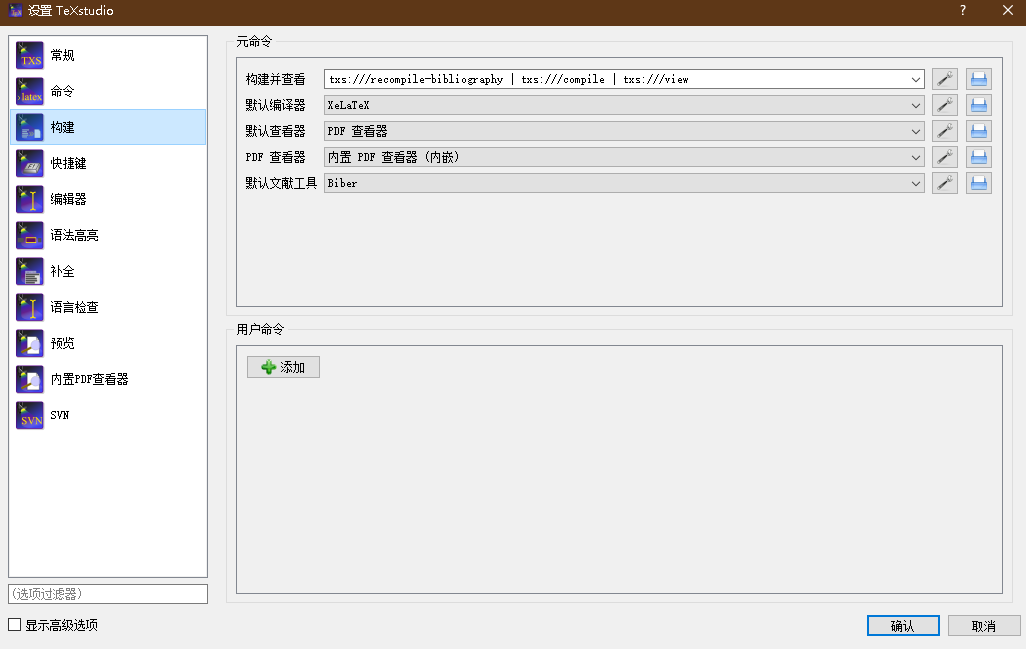
\includegraphics[scale=0.55]{Fig/TeXstudio.png}
	\caption{\label{TeXstudio}TeXstudio环境}
\end{figure}
\begin{figure}[htbp]
	\centering
	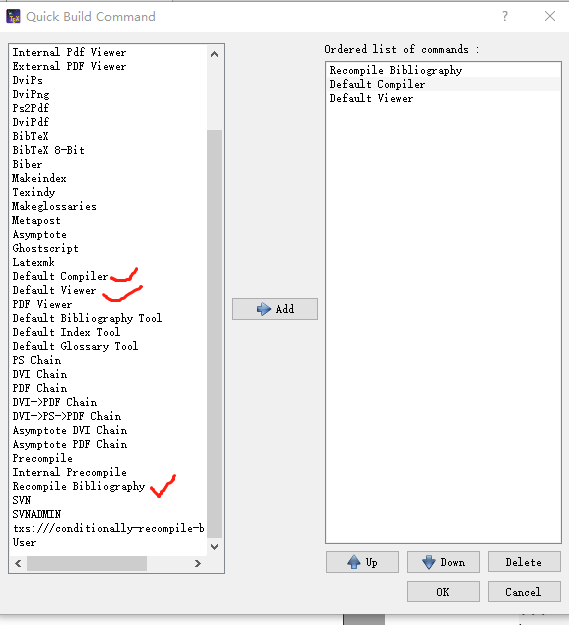
\includegraphics[scale=0.55]{Fig/setup.png}
	\caption{\label{setup}TeXstudio编译选项}
\end{figure}

\section{主文件}
gxuthesis.tex文件相当于主函数,调用各章的内容。\LaTeX{}源代码以一个\textbackslash{}documentclass 命令作为开头,它指定了文档使用的文档类。文档类规定了\LaTeX{}源代码所要生成的文档的性质——普通文章、书籍、演示文稿、个人简
历等等。
\begin{lstlisting}
\documentclass[<options>]{<class-name>}
\end{lstlisting}
其中class-name为文档类的名称,如\LaTeX{}提供的article, book, report,可在其基础上派
生的一些文档类或者有其它功能的一些文档类。\LaTeX{}提供的基础文档类见文献\parencite{_c}。还可以自定义文档类,如华南理工大学硕博士论文文档类gxuthesis,其实现保存在后缀名为.cls的文件中。可选参数options 为文档类指定选项。


document环境当中的内容是文档正文:
\begin{lstlisting}
\begin{document}
正文内容
\end{document}
\end{lstlisting}
正文中包含各章节内容:
\begin{lstlisting}
\chapter{摘\texorpdfstring{\quad}{}要}
	本模板由mengchaoheng\cite{_}开源的祖传华南理工大学硕/博士毕业论文Latex模型修改而来,旨在制作适合于广西大学硕/博士毕业论文Latex模型。

\keywordsCN{\LaTeX{};论文}

\chapter{Abstract}
	

\keywordsEN{\LaTeX{}; Paper} % 中英文摘要
\tableofcontents	% 目录
\listoftables	% 表格目录(可选)
\listoffigures	% 插图目录(可选)
\chapter{主要符号对照表}
【本节论文规范为可选,如果你的论文没有相关内容那么去除这一节;如果有,则删除这一行注释。】
\begin{table}
	\centering{}%
	\begin{tabular}{l>{\centering}p{0.5cm}l}
	 $ \boldsymbol{X}_n\boldsymbol{Y}_n\boldsymbol{Z}_n $-地理坐标系           &  & ${\boldsymbol{X}_b}{\boldsymbol{Y}_b}{\boldsymbol{Z}_b}$-机体坐标系\tabularnewline
	 $ \psi $-偏航角								   &  & $\theta$-俯仰角\tabularnewline
	 $\varphi$-滚转角  							   &  & $\boldsymbol{R}^n_b$、$\boldsymbol{R}$-机体系到NED系的旋转矩阵\tabularnewline
	 $\boldsymbol{G}$-NED系的重力  							  &  &   $\varphi_0 $-气动面安装角\tabularnewline
	 $ w $-系统的外部扰动								&  &  $T$-系统采样周期\tabularnewline
	 $\boldsymbol{F}$-机体系的气动力 						    &  &   $\boldsymbol{M}$-机体系的气动力矩\tabularnewline
	 $\rho$-空气密度 								  &  &  $C_{D,x} $、$ C_{D,y} $、$ C_{D,z} $-沿机体轴阻力系数\tabularnewline
	 $A_x $、$ A_y $、$ A_z $-沿机体轴的截面面积 		 &  &  $v$-机身相对于空气的速度分量\tabularnewline 
	 $l_{a}$-机身气动阻力作用点与重心的距离   			  &  &  $V_c$-气体在无穷远处的速度\tabularnewline
	 $T_d$-涵道体升力  								 &  &  $T_p$-风扇升力\tabularnewline
	 $T_a$-总升力 								      &  &  $q_a$-涵道升力分配系数\tabularnewline
	 $ p_U $-桨盘上表面压强 						   &  &  $p_L$-桨盘下表面压强\tabularnewline
	 $V_c+V_i$-桨盘上下表面气体速度 					 &  &  $S$-桨盘面积\tabularnewline
	 $ V_i $-桨盘处气流诱导速度 						  &  &  $ V_{cr} $-理想自转下降速率\tabularnewline
	 $ Q $-风扇扭矩 								 &  &  $ \varpi $-风扇转速\tabularnewline
	 $\mu$-环绕涵道角度变量 						  &  &  $\hat{\boldsymbol{i}}$-沿机体系$x$轴方向的单位矢量\tabularnewline 
	 $\hat{\boldsymbol{j}}$-沿机体系$y$轴方向的单位矢量  	   &  &  $C_{l, d}(\alpha_d)$-涵道翼型升力曲线\tabularnewline 
	 $C_{d, d}(\alpha_d)$涵道翼型阻力曲线  		      &  &  $c_d$-涵道翼型弦长\tabularnewline 
	 $C_{l_{\alpha}}$-风管翼型升力曲线斜率  			 &  &  $C_{l, \min }$、$ C_{l, \max } $-升力系数极限\tabularnewline 
	 $C_{d, o }$、$C_{d, g }$-拟合阻力曲线经验常数 	&  &  $R$-风扇半径\tabularnewline 
	 $C_{d u c t}$ - 常值比例系数  					&  &  $l_{d}$-重心与涵道气动力作用点的距离\tabularnewline
	 $k_{\delta}$-操纵面气动升力系数 				 &  &  $\alpha_d$-攻角\tabularnewline
	 $ I_{b}$-风扇转动惯量  						   &  &  $ d_{af} $ 、$ d_{ds} $-风扇扭矩常系数\tabularnewline
	 $\boldsymbol{L}_{{r}}$-风扇角动量  						&  & \tabularnewline 					
	\end{tabular}
\end{table}	% 符号对照表(可选)
\chapter{英文缩略词}
【本节论文规范为可选,如果你的论文没有相关内容那么去除这一节;如果有,则删除这一行注释。】
\begin{table}
	\centering{}%
	\begin{tabular}{ccc}
		SCUT  & South China University of Technology & 华南理工大学\tabularnewline
		&  & \tabularnewline
		&  & \tabularnewline
		&  & \tabularnewline
		&  & \tabularnewline
	\end{tabular}
\end{table} 	% 缩略词	
...
\chapter{绪论}
%
\section{研究背景和意义}
\subsection{研究背景和意义}
%
关于\LaTeX{}以及基于\LaTeX{}写作的好处不再赘述。\LaTeX{}的入门资料推荐文献\parencite{_g}以及文献\parencite{_c}。

这里主要是想推荐一种“学术生态”,即利用各种工具展开科研工作,以达到事半功倍的效果。需要用到以下软件:
\begin{enumerate}[topsep = 0 pt, itemsep= 0 pt, parsep=0pt, partopsep=0pt, leftmargin=44pt, itemindent=0pt, labelsep=6pt, label=(\arabic*)]
	\item 	参考文献管理软件zotero\cite{_m}。很多人使用过endnote,但其实zotero也非常强大,强烈推荐。可到b站观看Struggle with Me出品的视频教程\cite{_k}入门(或其他最新教程,刚开始不推荐使用插件,会增加学习难度)。zotero自带pdf阅读器,也可以设置为使用其他阅读器。在zotero可以打开文件所在位置,故不推荐更改zotero的文件系统(尤其不推荐使用zotfile插件,事实上各种五花八门的插件增加了复杂性,实际上没有带来太多便利性)。理论上只需要包含文献元数据信息的bib文件(可以手动一篇一篇文章地收集)即可使用此模板,因此模板不依赖于任何参考文献管理软件,endnote用户或不使用参考文献管理软件的用户可以忽略本文zotero部分的讲解。
	\item	可截图获取文献中公式的软件mathpix\cite{_h}。在阅读别人的论文时,很可能需要把文章中的公式抄下来放到自己的笔记中,方便以后组会报告甚至论文中使用,这时使用mathpix可直接截图获取\LaTeX{}源码,非常方便。随着mathpix的使用成本越来越高,免费次数越来越少,2023起已经不再推荐。目前开源/免费的替代工具为:\href{https://www.simpletex.cn/}{SimpleTex}和\href{https://p2t.breezedeus.com/}{Pix2Tex}。现在(2025年)SimpleTex网页不收费但客户端早已经收费,Pix2Tex虽然一般般但是好过没有,还是不错的选择,毕竟一般来说公式不会太复杂。Pix2Tex也一直在改进,可以本地部署也可以在线使用,MacOS还有桌面应用程序。
	\item	TeXlive202x、TeXstudio(2022起推荐vscode),相当于开发环境和IDE。本模板是基于TeX的发行版TeXlive202x和编辑器TeXstudio进行的,百度这两个关键字分别安装。关于TeXstudio的使用(快捷键等)可另行查找资料。模板还支持更多ide,更多编译方式见GitHub首页readme.md。若在其他窗口打开了编译生成的pdf文件,记得关掉再编译,否则报错。TeXstudio的设置见第二章。vscode的设置见github讨论区的\href{https://github.com/mengchaoheng/SCUT_thesis/discussions/6}{vscode配置}。
\end{enumerate}

本文的章节安排如下:

第一章,绪论。

第二章,模板简介。主要介绍各文件的内容。

第三章,常用环境。介绍论文写作中常用的环境,包括:图、表、公式、定理。基本涵盖了常用的命令。

%第三章,参考文献设置。本模板对旧版的改动主要是参考文献部分,本章将简单参考文献设置以及
%编译选项的设置等等。


	% 第一章
\chapter{模板简介}
%
与很多外文杂志社不同,大部分中文期刊都不提供\LaTeX{}模板给投稿者使用,也很少有学校给学生提供官方的毕业论文模板。目前github上的大部分模板都是由学生发起的非官方模板。在此感谢Shun Xu以及yecfly等人的工作,他们的无私贡献使得华南理工大学硕博士毕业论文也可以使用\LaTeX{}撰写。

本模板是直接修改前人的模板得到的,更详细的介绍可到\parencite{_,_a}下载。本章仅从用户的角度简要介绍模板的使用,而尽量避免涉及\LaTeX{}的模板制作细节(实际上是因为本人也不会)。正如我们使用手机并不需要了解麦克斯韦方程组,使用\LaTeX{}写作也无需了解模板是如何制作的。

\LaTeX{}的源代码保存在后缀名为.tex的文件中。当编写长篇文档时,例如当编写书籍、毕业论文时,单个源文件会使修改、校对变得十分困
难。将源文件分割成若干个文件,例如将每章内容单独写在一个文件中,会大大简化修改和校对
的工作。为方便,本文将gxuthesis.tex文件称为主文件,而将chapter文件夹的abstract.tex、chapter0x.tex、conclusion.tex等文件称为章节文件。

值得注意的是,要每次编译时都更新参考文献著录,TeXstudio软件的选项->设置中的构建并查看、编译器需要设置成如图\ref{TeXstudio}、\ref{setup}所示。此时只需在任意一个文件中点击构建并查看按钮即可编译文档。每次编译都更新参考文献会使得编译时间很长。
\begin{figure}[htbp]
	\centering
	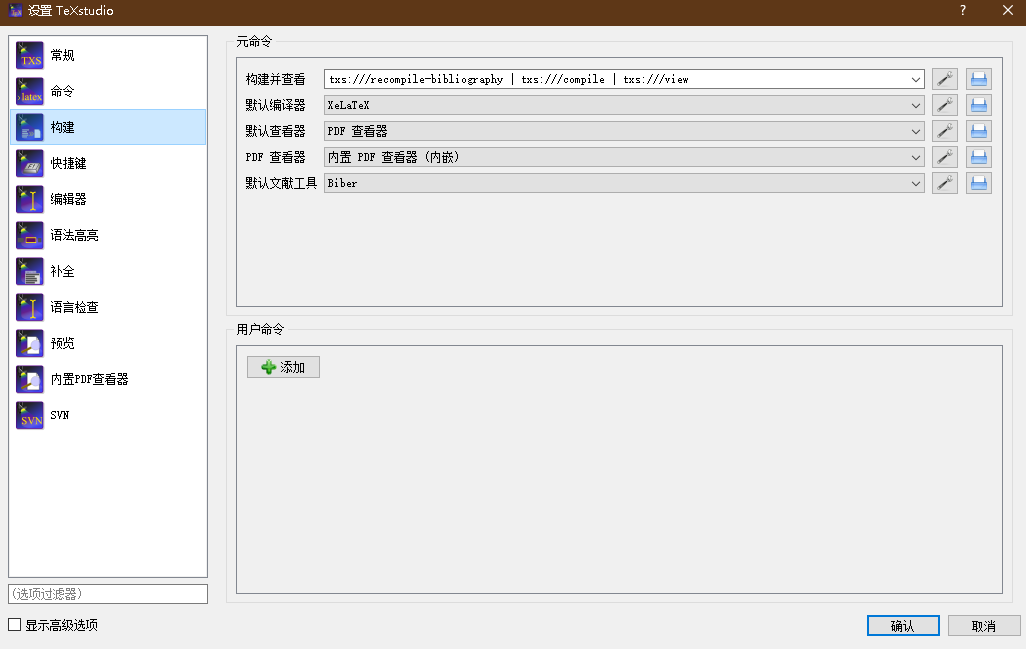
\includegraphics[scale=0.55]{Fig/TeXstudio.png}
	\caption{\label{TeXstudio}TeXstudio环境}
\end{figure}
\begin{figure}[htbp]
	\centering
	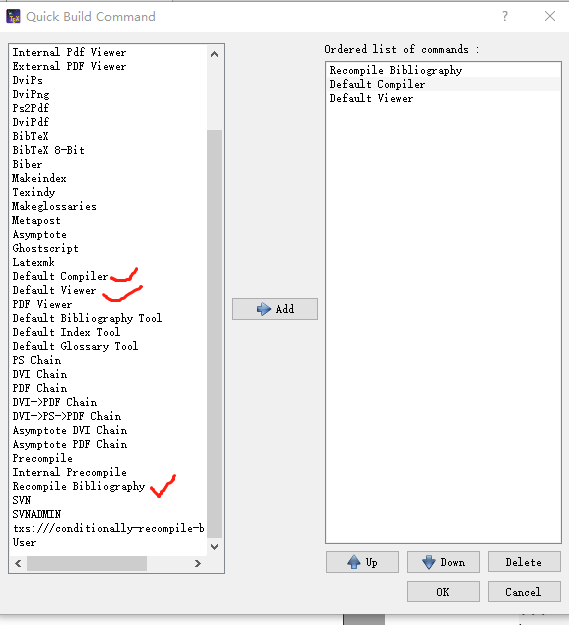
\includegraphics[scale=0.55]{Fig/setup.png}
	\caption{\label{setup}TeXstudio编译选项}
\end{figure}

\section{主文件}
gxuthesis.tex文件相当于主函数,调用各章的内容。\LaTeX{}源代码以一个\textbackslash{}documentclass 命令作为开头,它指定了文档使用的文档类。文档类规定了\LaTeX{}源代码所要生成的文档的性质——普通文章、书籍、演示文稿、个人简
历等等。
\begin{lstlisting}
\documentclass[<options>]{<class-name>}
\end{lstlisting}
其中class-name为文档类的名称,如\LaTeX{}提供的article, book, report,可在其基础上派
生的一些文档类或者有其它功能的一些文档类。\LaTeX{}提供的基础文档类见文献\parencite{_c}。还可以自定义文档类,如华南理工大学硕博士论文文档类gxuthesis,其实现保存在后缀名为.cls的文件中。可选参数options 为文档类指定选项。


document环境当中的内容是文档正文:
\begin{lstlisting}
\begin{document}
正文内容
\end{document}
\end{lstlisting}
正文中包含各章节内容:
\begin{lstlisting}
\chapter{摘\texorpdfstring{\quad}{}要}
	本模板由mengchaoheng\cite{_}开源的祖传华南理工大学硕/博士毕业论文Latex模型修改而来,旨在制作适合于广西大学硕/博士毕业论文Latex模型。

\keywordsCN{\LaTeX{};论文}

\chapter{Abstract}
	

\keywordsEN{\LaTeX{}; Paper} % 中英文摘要
\tableofcontents	% 目录
\listoftables	% 表格目录(可选)
\listoffigures	% 插图目录(可选)
\chapter{主要符号对照表}
【本节论文规范为可选,如果你的论文没有相关内容那么去除这一节;如果有,则删除这一行注释。】
\begin{table}
	\centering{}%
	\begin{tabular}{l>{\centering}p{0.5cm}l}
	 $ \boldsymbol{X}_n\boldsymbol{Y}_n\boldsymbol{Z}_n $-地理坐标系           &  & ${\boldsymbol{X}_b}{\boldsymbol{Y}_b}{\boldsymbol{Z}_b}$-机体坐标系\tabularnewline
	 $ \psi $-偏航角								   &  & $\theta$-俯仰角\tabularnewline
	 $\varphi$-滚转角  							   &  & $\boldsymbol{R}^n_b$、$\boldsymbol{R}$-机体系到NED系的旋转矩阵\tabularnewline
	 $\boldsymbol{G}$-NED系的重力  							  &  &   $\varphi_0 $-气动面安装角\tabularnewline
	 $ w $-系统的外部扰动								&  &  $T$-系统采样周期\tabularnewline
	 $\boldsymbol{F}$-机体系的气动力 						    &  &   $\boldsymbol{M}$-机体系的气动力矩\tabularnewline
	 $\rho$-空气密度 								  &  &  $C_{D,x} $、$ C_{D,y} $、$ C_{D,z} $-沿机体轴阻力系数\tabularnewline
	 $A_x $、$ A_y $、$ A_z $-沿机体轴的截面面积 		 &  &  $v$-机身相对于空气的速度分量\tabularnewline 
	 $l_{a}$-机身气动阻力作用点与重心的距离   			  &  &  $V_c$-气体在无穷远处的速度\tabularnewline
	 $T_d$-涵道体升力  								 &  &  $T_p$-风扇升力\tabularnewline
	 $T_a$-总升力 								      &  &  $q_a$-涵道升力分配系数\tabularnewline
	 $ p_U $-桨盘上表面压强 						   &  &  $p_L$-桨盘下表面压强\tabularnewline
	 $V_c+V_i$-桨盘上下表面气体速度 					 &  &  $S$-桨盘面积\tabularnewline
	 $ V_i $-桨盘处气流诱导速度 						  &  &  $ V_{cr} $-理想自转下降速率\tabularnewline
	 $ Q $-风扇扭矩 								 &  &  $ \varpi $-风扇转速\tabularnewline
	 $\mu$-环绕涵道角度变量 						  &  &  $\hat{\boldsymbol{i}}$-沿机体系$x$轴方向的单位矢量\tabularnewline 
	 $\hat{\boldsymbol{j}}$-沿机体系$y$轴方向的单位矢量  	   &  &  $C_{l, d}(\alpha_d)$-涵道翼型升力曲线\tabularnewline 
	 $C_{d, d}(\alpha_d)$涵道翼型阻力曲线  		      &  &  $c_d$-涵道翼型弦长\tabularnewline 
	 $C_{l_{\alpha}}$-风管翼型升力曲线斜率  			 &  &  $C_{l, \min }$、$ C_{l, \max } $-升力系数极限\tabularnewline 
	 $C_{d, o }$、$C_{d, g }$-拟合阻力曲线经验常数 	&  &  $R$-风扇半径\tabularnewline 
	 $C_{d u c t}$ - 常值比例系数  					&  &  $l_{d}$-重心与涵道气动力作用点的距离\tabularnewline
	 $k_{\delta}$-操纵面气动升力系数 				 &  &  $\alpha_d$-攻角\tabularnewline
	 $ I_{b}$-风扇转动惯量  						   &  &  $ d_{af} $ 、$ d_{ds} $-风扇扭矩常系数\tabularnewline
	 $\boldsymbol{L}_{{r}}$-风扇角动量  						&  & \tabularnewline 					
	\end{tabular}
\end{table}	% 符号对照表(可选)
\chapter{英文缩略词}
【本节论文规范为可选,如果你的论文没有相关内容那么去除这一节;如果有,则删除这一行注释。】
\begin{table}
	\centering{}%
	\begin{tabular}{ccc}
		SCUT  & South China University of Technology & 华南理工大学\tabularnewline
		&  & \tabularnewline
		&  & \tabularnewline
		&  & \tabularnewline
		&  & \tabularnewline
	\end{tabular}
\end{table} 	% 缩略词	
...
\chapter{绪论}
%
\section{研究背景和意义}
\subsection{研究背景和意义}
%
关于\LaTeX{}以及基于\LaTeX{}写作的好处不再赘述。\LaTeX{}的入门资料推荐文献\parencite{_g}以及文献\parencite{_c}。

这里主要是想推荐一种“学术生态”,即利用各种工具展开科研工作,以达到事半功倍的效果。需要用到以下软件:
\begin{enumerate}[topsep = 0 pt, itemsep= 0 pt, parsep=0pt, partopsep=0pt, leftmargin=44pt, itemindent=0pt, labelsep=6pt, label=(\arabic*)]
	\item 	参考文献管理软件zotero\cite{_m}。很多人使用过endnote,但其实zotero也非常强大,强烈推荐。可到b站观看Struggle with Me出品的视频教程\cite{_k}入门(或其他最新教程,刚开始不推荐使用插件,会增加学习难度)。zotero自带pdf阅读器,也可以设置为使用其他阅读器。在zotero可以打开文件所在位置,故不推荐更改zotero的文件系统(尤其不推荐使用zotfile插件,事实上各种五花八门的插件增加了复杂性,实际上没有带来太多便利性)。理论上只需要包含文献元数据信息的bib文件(可以手动一篇一篇文章地收集)即可使用此模板,因此模板不依赖于任何参考文献管理软件,endnote用户或不使用参考文献管理软件的用户可以忽略本文zotero部分的讲解。
	\item	可截图获取文献中公式的软件mathpix\cite{_h}。在阅读别人的论文时,很可能需要把文章中的公式抄下来放到自己的笔记中,方便以后组会报告甚至论文中使用,这时使用mathpix可直接截图获取\LaTeX{}源码,非常方便。随着mathpix的使用成本越来越高,免费次数越来越少,2023起已经不再推荐。目前开源/免费的替代工具为:\href{https://www.simpletex.cn/}{SimpleTex}和\href{https://p2t.breezedeus.com/}{Pix2Tex}。现在(2025年)SimpleTex网页不收费但客户端早已经收费,Pix2Tex虽然一般般但是好过没有,还是不错的选择,毕竟一般来说公式不会太复杂。Pix2Tex也一直在改进,可以本地部署也可以在线使用,MacOS还有桌面应用程序。
	\item	TeXlive202x、TeXstudio(2022起推荐vscode),相当于开发环境和IDE。本模板是基于TeX的发行版TeXlive202x和编辑器TeXstudio进行的,百度这两个关键字分别安装。关于TeXstudio的使用(快捷键等)可另行查找资料。模板还支持更多ide,更多编译方式见GitHub首页readme.md。若在其他窗口打开了编译生成的pdf文件,记得关掉再编译,否则报错。TeXstudio的设置见第二章。vscode的设置见github讨论区的\href{https://github.com/mengchaoheng/SCUT_thesis/discussions/6}{vscode配置}。
\end{enumerate}

本文的章节安排如下:

第一章,绪论。

第二章,模板简介。主要介绍各文件的内容。

第三章,常用环境。介绍论文写作中常用的环境,包括:图、表、公式、定理。基本涵盖了常用的命令。

%第三章,参考文献设置。本模板对旧版的改动主要是参考文献部分,本章将简单参考文献设置以及
%编译选项的设置等等。


	% 第一章
\chapter{模板简介}
%
与很多外文杂志社不同,大部分中文期刊都不提供\LaTeX{}模板给投稿者使用,也很少有学校给学生提供官方的毕业论文模板。目前github上的大部分模板都是由学生发起的非官方模板。在此感谢Shun Xu以及yecfly等人的工作,他们的无私贡献使得华南理工大学硕博士毕业论文也可以使用\LaTeX{}撰写。

本模板是直接修改前人的模板得到的,更详细的介绍可到\parencite{_,_a}下载。本章仅从用户的角度简要介绍模板的使用,而尽量避免涉及\LaTeX{}的模板制作细节(实际上是因为本人也不会)。正如我们使用手机并不需要了解麦克斯韦方程组,使用\LaTeX{}写作也无需了解模板是如何制作的。

\LaTeX{}的源代码保存在后缀名为.tex的文件中。当编写长篇文档时,例如当编写书籍、毕业论文时,单个源文件会使修改、校对变得十分困
难。将源文件分割成若干个文件,例如将每章内容单独写在一个文件中,会大大简化修改和校对
的工作。为方便,本文将gxuthesis.tex文件称为主文件,而将chapter文件夹的abstract.tex、chapter0x.tex、conclusion.tex等文件称为章节文件。

值得注意的是,要每次编译时都更新参考文献著录,TeXstudio软件的选项->设置中的构建并查看、编译器需要设置成如图\ref{TeXstudio}、\ref{setup}所示。此时只需在任意一个文件中点击构建并查看按钮即可编译文档。每次编译都更新参考文献会使得编译时间很长。
\begin{figure}[htbp]
	\centering
	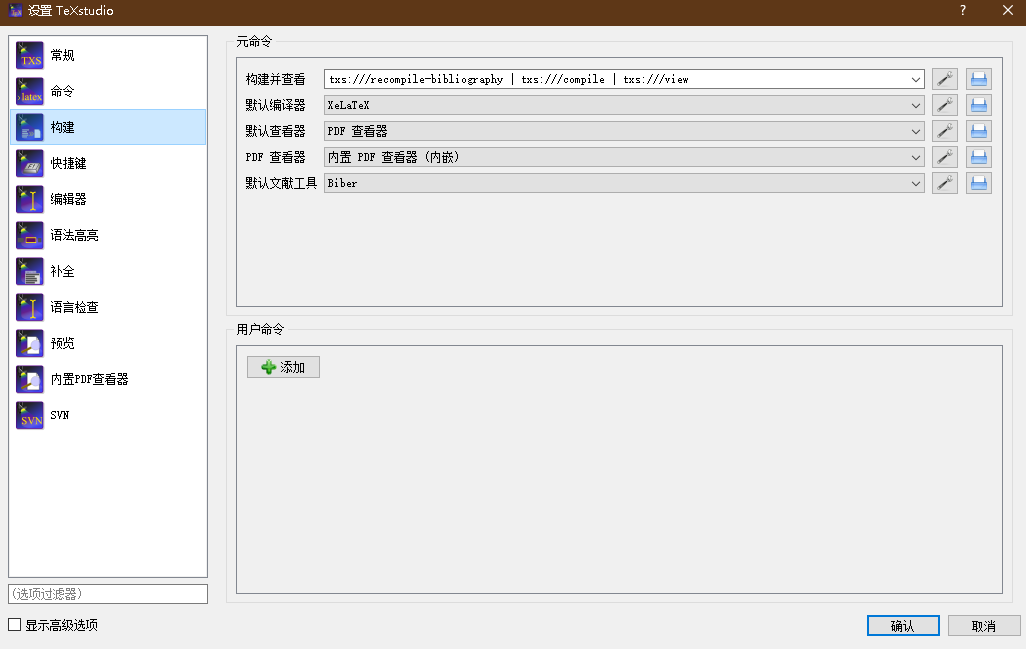
\includegraphics[scale=0.55]{Fig/TeXstudio.png}
	\caption{\label{TeXstudio}TeXstudio环境}
\end{figure}
\begin{figure}[htbp]
	\centering
	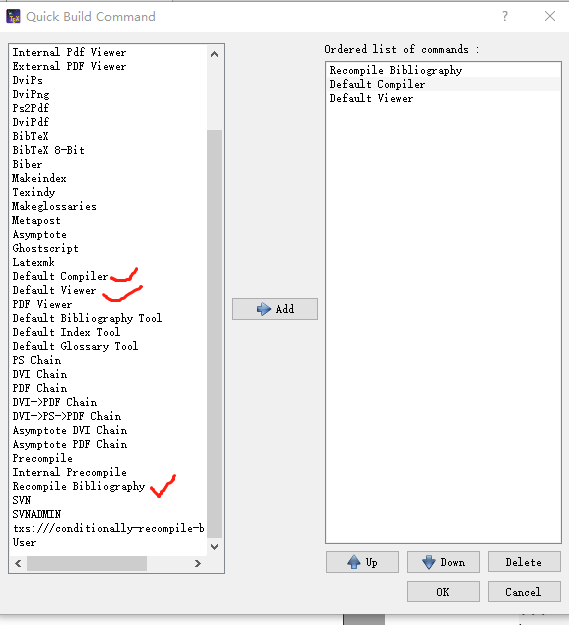
\includegraphics[scale=0.55]{Fig/setup.png}
	\caption{\label{setup}TeXstudio编译选项}
\end{figure}

\section{主文件}
gxuthesis.tex文件相当于主函数,调用各章的内容。\LaTeX{}源代码以一个\textbackslash{}documentclass 命令作为开头,它指定了文档使用的文档类。文档类规定了\LaTeX{}源代码所要生成的文档的性质——普通文章、书籍、演示文稿、个人简
历等等。
\begin{lstlisting}
\documentclass[<options>]{<class-name>}
\end{lstlisting}
其中class-name为文档类的名称,如\LaTeX{}提供的article, book, report,可在其基础上派
生的一些文档类或者有其它功能的一些文档类。\LaTeX{}提供的基础文档类见文献\parencite{_c}。还可以自定义文档类,如华南理工大学硕博士论文文档类gxuthesis,其实现保存在后缀名为.cls的文件中。可选参数options 为文档类指定选项。


document环境当中的内容是文档正文:
\begin{lstlisting}
\begin{document}
正文内容
\end{document}
\end{lstlisting}
正文中包含各章节内容:
\begin{lstlisting}
\include{abstract} % 中英文摘要
\tableofcontents	% 目录
\listoftables	% 表格目录(可选)
\listoffigures	% 插图目录(可选)
\include{symbols}	% 符号对照表(可选)
\include{abbreviation} 	% 缩略词	
...
\include{chapter01}	% 第一章
\include{chapter02} % 第二章
\include{chapter03} % 第三章
% 自行根据需要添加章节。
...
\include{conclusion} % 结论
...
\printbibliography	% 参考文献著录
\include{appendix} % 附录
\include{pub} % 成果
\include{ack} % 致谢
\end{lstlisting}
其中$\%$之后的内容为注释,...表示省略其他代码,仅保留论文内容主体部分。\textbackslash{}include\{xxx\}指令用于包含xxx.tex文件的内容,各章节的内容主要在xxx.tex中保存。在\textbackslash{}documentclass 和\textbackslash{}begin\{document\} 之间的位置称为导言区。在导言区中一般会使用\textbackslash{}usepackage 调用宏包,以及会进行对文档的全局设置。本模板的导言区除调用所需的宏包外,还进行了页眉页脚的设置。有的模板会把所有调用宏包的指令放到一个.sty宏包文件中,页面的设置放在文档类文件.cls文件中。因本人时间有限,就不做整理,欢迎有志之士加入完善。使用本模板并不需要了解导言区的指令,在需要时额外添加即可(要注意宏包冲突)。特别地,\textbackslash{}includeonly\{xxx\}指令用于使文档仅编译xxx.tex文件的内容,这就是分章节包含(include)的好处,可大大减少编译时间。

将封面打印保存为 thesis\_cover.pdf 文件,硕士使用master\_cover.docx ,博士使用 doctor\_cover.doc 。如果有更新版本的封面,可自行替换。文档类默认是博士论文,下面指令将控制添加封面与否:
\begin{lstlisting}
\documentclass[unicode,master,pdfcover]{gxuthesis}	% 使用pdf文件封面的 硕士模板
\documentclass[unicode,master]{gxuthesis}	% 不使用pdf文件封面的 硕士模板
\documentclass[unicode,pdfcover]{gxuthesis}	% 使用pdf文件封面的博士模板
\documentclass[unicode]{gxuthesis}	% 不使用pdf文件封面的博士模板
\end{lstlisting}
不使用thesis\_cover.pdf 文件指定的封面时,将使用草稿封面。草稿封面也可以减少编译时间,因此可以在最终提交论文时再使用论文封面。草稿封面用以下指令设置:
\begin{lstlisting}
%%%%%%%%%%%%%草稿封面设置%%%%%%%%%%%%%	
\title{LaTeX模板}	
\author{作者姓名}	
\supervisor{指导教师:xxx\ 教授}	
\institute{华南理工大学}	
\date{2020年5月20日}
%%%%%%%%%%%%%%%%%%%%%%%%%%%%%%%%%%%%%
\end{lstlisting}
\section{章节文件}
chapter文件夹的章节文件如chapter0x.tex等,其内容由\textbackslash{}chapter\{章名\}开头。新建一章可新建一个文件并由\textbackslash{}chapter\{新建章名\}开头填写内容即可。节及小节分别用\textbackslash{}section\{新建节名\}、\textbackslash{}subsection\{新建小节名\}命令。

正文的的书写和txt文本文件的书写类似。\LaTeX{} 源代码中,空格键和Tab键输入的空白字符视为“空格”。连续的若干个空白字符视为一个空格。一行开头的空格忽略不计。行末的回车视为一个空格;但连续两个回车,也就是空行,会将文字分段。多个空行被视为一个空行。也可以在行末使用\textbackslash{}par 命令分段。在本模板中,英文之间的空格被保留,中文之间的空格被忽略。特别地,摘要,附录,结论等两个字的大纲级别为章的章名,中间使用空格隔开。对此论文撰写规范并没有明文要求,只是为了美观。也可以全部不加空格。一般情况下,在文本文字中添加空格使用\textbackslash{}quad命令,但由于文献\parencite{_d}所述原因,直接使用\textbackslash{}quad命令会报警,因而使用\textbackslash{}texorpdfstring\{\textbackslash{}quad\}\{\},其中最后一个\{\}里面可以加一个空格,不影响使用。目录二字之间添加空格在gxuthesis.cls文件317行设置。

正文本环境中使用公式,即行内公式,需要用两个\$包围,如源码:\$a+b=c\$ 显示为$a+b=c$。使用其他字符可自行百度或阅读参考文献。再次提醒,使用\LaTeX{}撰写论文不需要研究其原理,在达到某种效果(图文显示、公式显示效果)时百度或查书寻找其代码即可。

综上,论文撰写只需要将自己的文本(包含行内公式)放到相应的章节处,并添加行间公式、图表环境并填写图表即可。行间公式、图表将在下一章介绍。

 % 第二章

\chapter{常用环境及参考文献设置}
强烈建议在使用公式、表格、定理环境时进行百度,没必要研究各种用法,只需要知道自己需要什么。因本人的论文所用表格较少,因而对表格不是很熟悉,本章对表格的介绍相应的较少。本章仅介绍本人在论文撰写过程中常用的环境以及参考文献设置。

\section{图}
图的导入需要提前准备好图片文件,最好是.png、.eps、.pdf或.jpg文件。另外,如果是从matlab导出图片文件,可使用print函数或手动导出,print函数的使用可参考ICGNC2020plot.m以及PlotToFileColorPDF.m文件等。手动导出(matlab的figure界面的“文件”->“导出设置”设置好大小、分辨率和线宽等然后点击“应用于图窗”)主要用于观察效果,可设置某种样式名称后保存该样式,下次使用时加载,具体可百度“matlab导出高清图片”。需要特别注意的是一定要1:1导入matlab生成的图片,并且图中文字设置好字体字号。否则缩放之后,图片的字号就变了,盲审老师一眼就能看出来字号不对,就很麻烦。这就是为什么要在matlab点击“应用于图窗“进行预览,观测效果后再1:1使用图片。

使用如下代码放置独立成行的图片,效果如图\ref{one_DFUAV}所示
\begin{lstlisting}
\begin{figure}[htbp]
	% 图片居中(列居中对齐)
	\centering	
	% 包含当前路径下的Fig文件夹的图片文件DFUAV_f31.png
	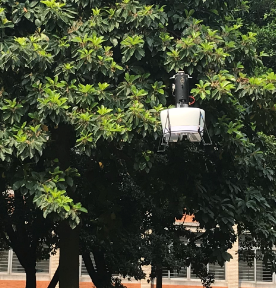
\includegraphics[scale=1]{Fig/DFUAV_f31.png} 
	% 添加标签one_DFUAV以及图标题“涵道风扇式无人机”,引用某图时使用\ref{xxx},其中xxx就是标签,图编号是自动生成的。
	\caption{\label{one_DFUAV}涵道风扇式无人机} 
\end{figure}
\end{lstlisting}
其中figure为环境名,[htbp]表示将图片设置为浮动体,实际上这在.cls文件已经设置过,因而可以省略。[scale=1]表示安装1:1的比例导入图片,还可以按其他方式导入,需要时可自行百度。
\begin{figure}[htbp]
	\centering
	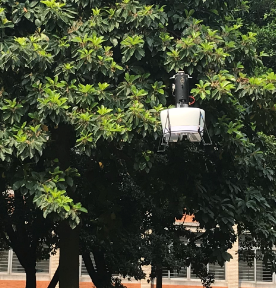
\includegraphics[scale=1]{Fig/DFUAV_f31.png}
	\caption{\label{one_DFUAV}涵道风扇式无人机}
\end{figure}

使用如下代码划分页面并排放置图\ref{Hawk}、图\ref{GTSpy}
\begin{lstlisting}
\begin{figure}[htbp]
	\centering
	\begin{minipage}[c]{0.5\textwidth} % minipage将页面划分为0.5\textwidth
		\centering
		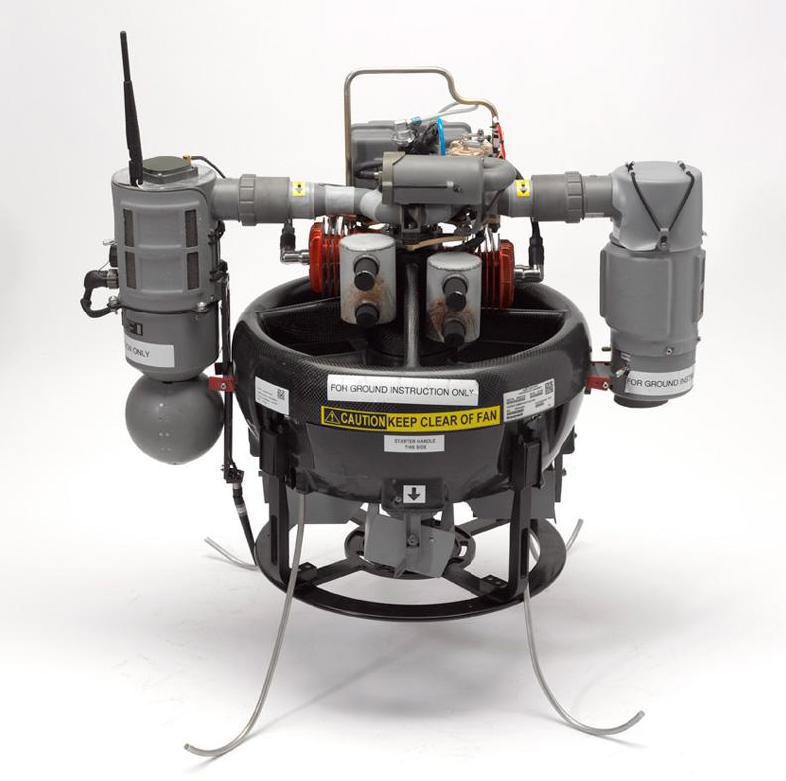
\includegraphics[width=6cm,height=6cm]{Fig/honeywell_t-hawk.jpg}
		\caption{\label{Hawk}T-Hawk}
	\end{minipage}%
	\begin{minipage}[c]{0.5\textwidth}
		\centering
		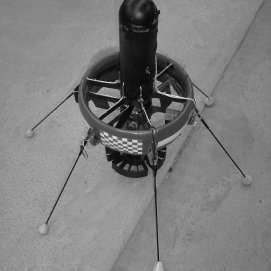
\includegraphics[width=6cm,height=6cm]{Fig/GTSpy.jpg}
		\caption{\label{GTSpy}GTSpy}
	\end{minipage}
\end{figure}
\end{lstlisting}
其中[c]表示行居中对齐。当图片大小不一但又需要1:1导入时,图标题可能行不对齐,因此可以改为如下指令:
\begin{lstlisting}
\begin{figure}[htbp]
	\centering
	\begin{minipage}[c]{0.5\textwidth}
		\centering
		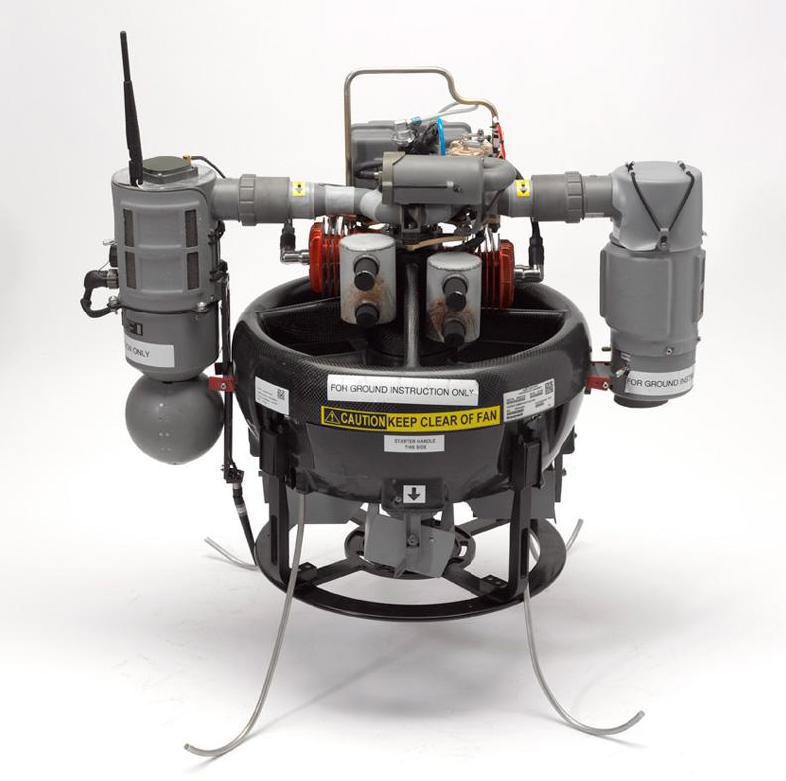
\includegraphics[scale=1]{Fig/honeywell_t-hawk.jpg} %1:1导入
	\end{minipage}%
	\begin{minipage}[c]{0.5\textwidth}
		\centering
		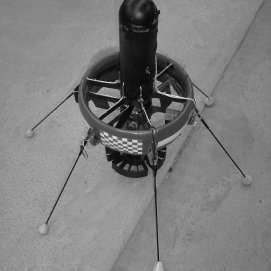
\includegraphics[scale=1]{Fig/GTSpy.jpg}
	\end{minipage}\\[1pt]
	\begin{minipage}[t]{0.5\textwidth}	% 以下为新添加页面划分,[t]表示行顶部对齐
		\caption{\label{Hawk}T-Hawk}
	\end{minipage}%
	\begin{minipage}[t]{0.5\textwidth}
		\caption{\label{GTSpy}GTSpy}
	\end{minipage}%
\end{figure}
\end{lstlisting}
\begin{figure}[htbp]
	\centering
	\begin{minipage}[c]{0.5\textwidth}
		\centering
		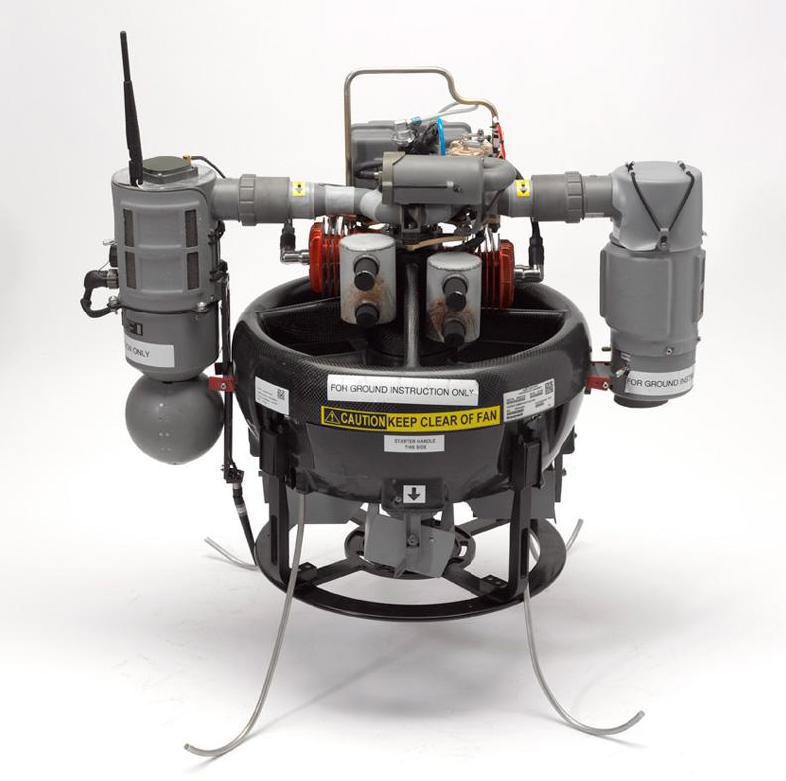
\includegraphics[width=6cm,height=6cm]{Fig/honeywell_t-hawk.jpg}
		\caption{\label{Hawk}T-Hawk}
	\end{minipage}%
	\begin{minipage}[c]{0.5\textwidth}
		\centering
		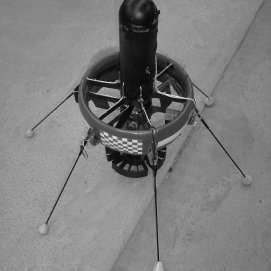
\includegraphics[width=6cm,height=6cm]{Fig/GTSpy.jpg}
		\caption{\label{GTSpy}GTSpy}
	\end{minipage}
\end{figure}


通常一个figure内含有其他小的figure,可以使用一些宏包,但最初本着简单的原则,本模板并没有使用这些子图包。后来应同学们要求在,把子图的功能加上,主要是修改了模板文件(gxuthesis.cls文件)的功能包参数。注意,很多网上拿到的代码不一定可以精确的调子图标题字体字号,因为此模板的子图标题字体字号是利用subfig宏包的选项进行设置的(在gxuthesis.cls文件的“图表环境”中),而有些教程使用subcaption进行同样的设置,还需进一步验证可行性。另外图的排版方法很多,有些宏包已经被弃用,所以尽量使用本文给出的案例的格式进行排版图片。

常见的子图包有subfigure和subfig。subfigure是比较老的了,这里使用subfig包。两个包在使用的时候用法不同,千万不要混淆了,不然可能会报错。subfig包的命令是\textbackslash{}subfloat。这里给出一种使用subfig包的常用排版,如图\ref{Fig:1}的子图\subref{Fig:1:b},其中\subref*{Fig:1:a}的试验并不好(这里测试了交叉引用\textbackslash{}subref\{xxx\}和\textbackslash{}subref*\{xxx\})。必要时也可以排版多行多列的图、调整图之间的间距,具体可百度。

\begin{lstlisting}
\begin{figure}[!h]
	\centering
	\subfloat[不合理的轨迹]{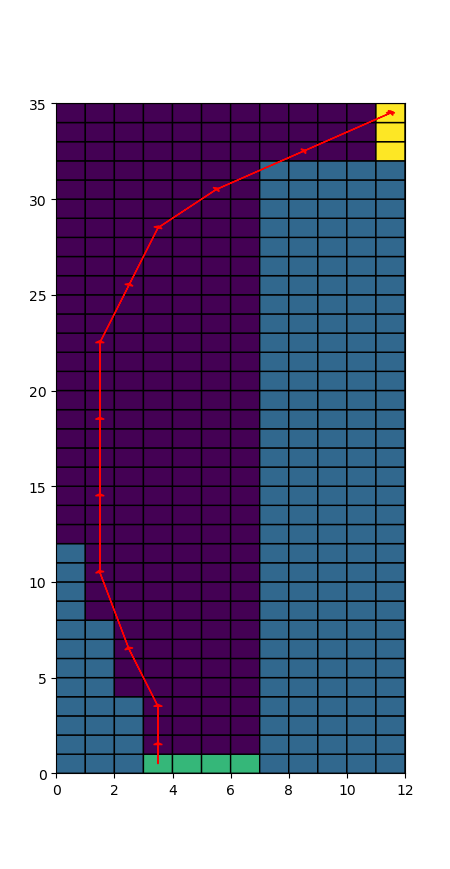
\includegraphics[width=6cm,height=6cm]{Fig/Figure_1.png}%
		\label{Fig:1:a}}
	\subfloat[优化的轨迹]{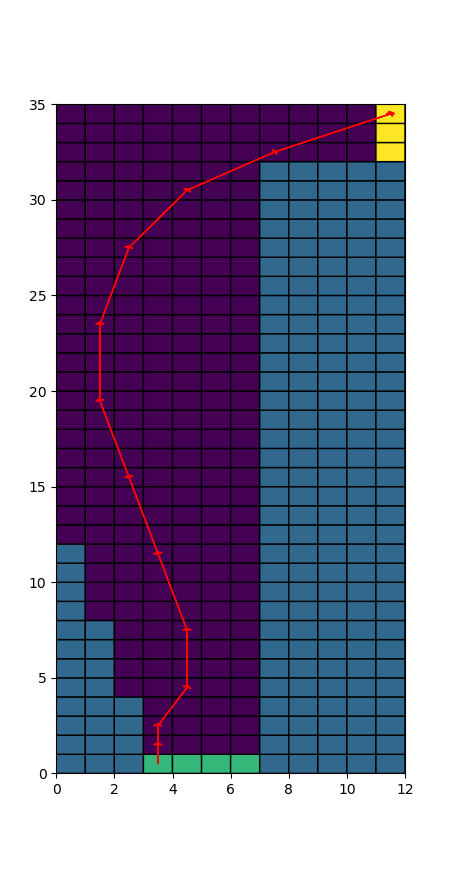
\includegraphics[width=6cm,height=6cm]{Fig/Figure_2.png}
		\label{Fig:1:b}}
	\\ % 用 \\ 换行,也可以此处空一行进行换行,只有两个图的话下面就不需要了。
	\subfloat[不合理的轨迹]{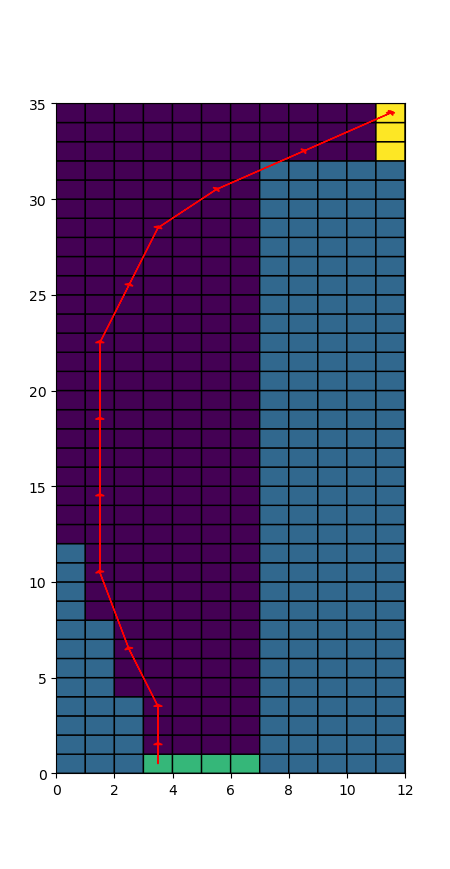
\includegraphics[width=6cm,height=6cm]{Fig/Figure_1.png}%
		\label{Fig:1:c}}
	\subfloat[优化的轨迹]{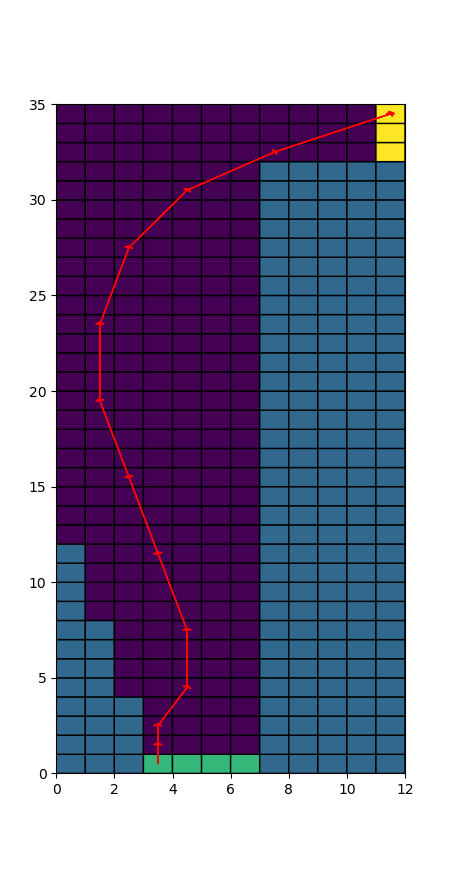
\includegraphics[width=6cm,height=6cm]{Fig/Figure_2.png}%
		\label{Fig:1:d}}
	\caption{子图包使用测试}\label{Fig:1}
\end{figure}
----------------------------------------------------------
% 引用某子图时使用\subref{xxx},其中xxx就是标签Fig:1:a
子图的引用比较特殊,命令有:\subref{xxx}和\subref*{xxx}
注:在subfig包使用说明中,\subref{xxx}和\subref*{xxx}分别由参数listofformat和subrefformat控制,
并由如下定义,根据撰写规范需要定义为:
\DeclareSubrefFormat{empty}{}
\DeclareSubrefFormat{simple}{#1#2}
\DeclareSubrefFormat{parens}{#1 #2)}
\DeclareSubrefFormat{subsimple}{#2}
\DeclareSubrefFormat{subparens}{ #2)}
和
\DeclareCaptionListOfFormat{empty}{}
\DeclareCaptionListOfFormat{simple}{#1#2}
\DeclareCaptionListOfFormat{parens}{#1 #2)}
\DeclareCaptionListOfFormat{subsimple}{#2}
\DeclareCaptionListOfFormat{subparens}{ #2)}
\end{lstlisting}
\begin{figure}[!h]
	\centering
	\subfloat[不合理的轨迹]{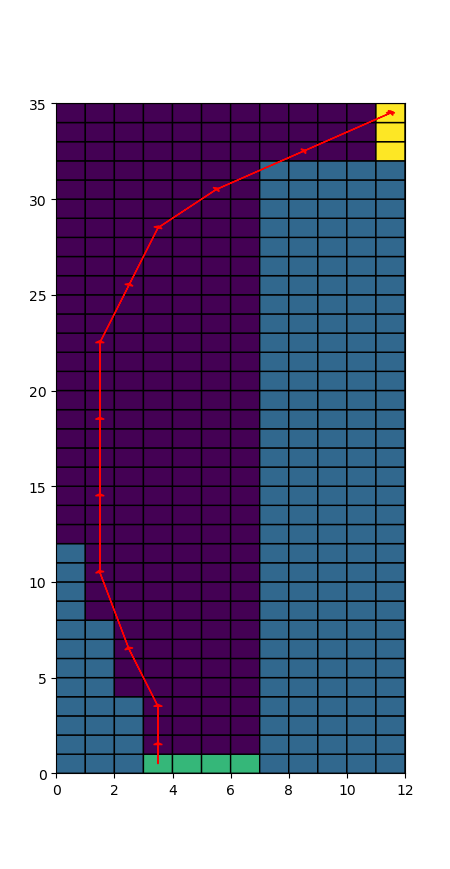
\includegraphics[width=6cm,height=6cm]{Fig/Figure_1.png}%
		\label{Fig:1:a}}
	\subfloat[优化的轨迹]{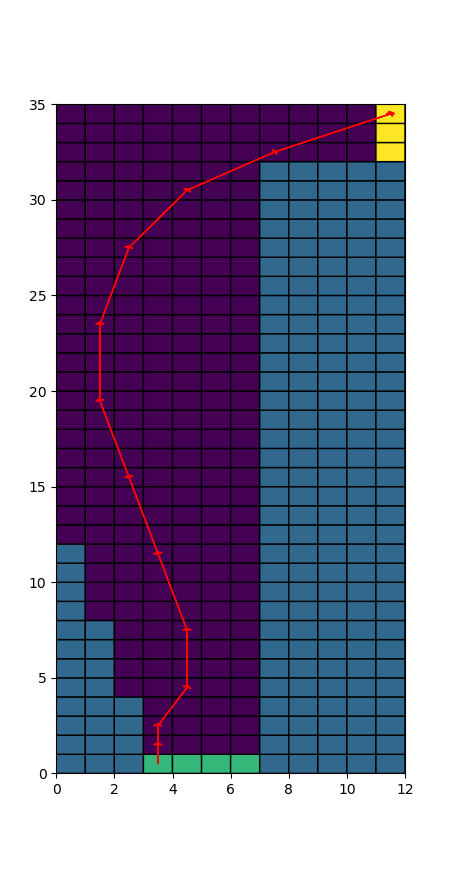
\includegraphics[width=6cm,height=6cm]{Fig/Figure_2.png}
 		\label{Fig:1:b}}
	\\ % 用 \\ 换行,也可以此处空一行进行换行
	\subfloat[不合理的轨迹]{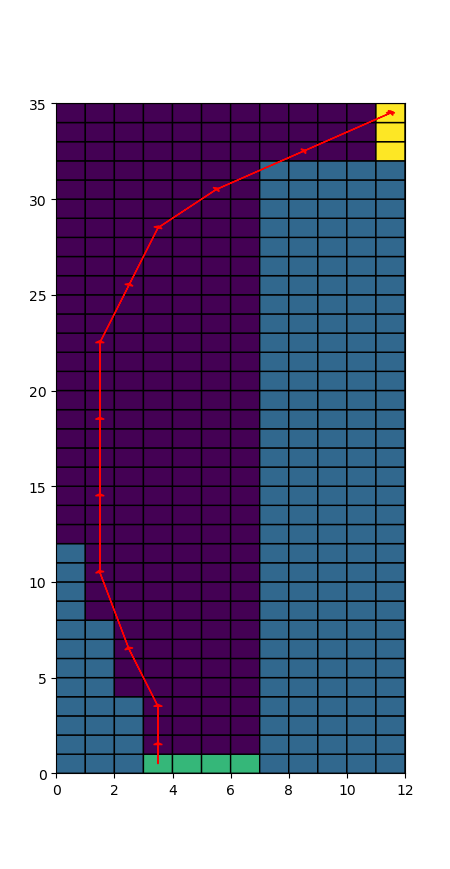
\includegraphics[width=6cm,height=6cm]{Fig/Figure_1.png}%
		\label{Fig:1:c}}
	\subfloat[优化的轨迹]{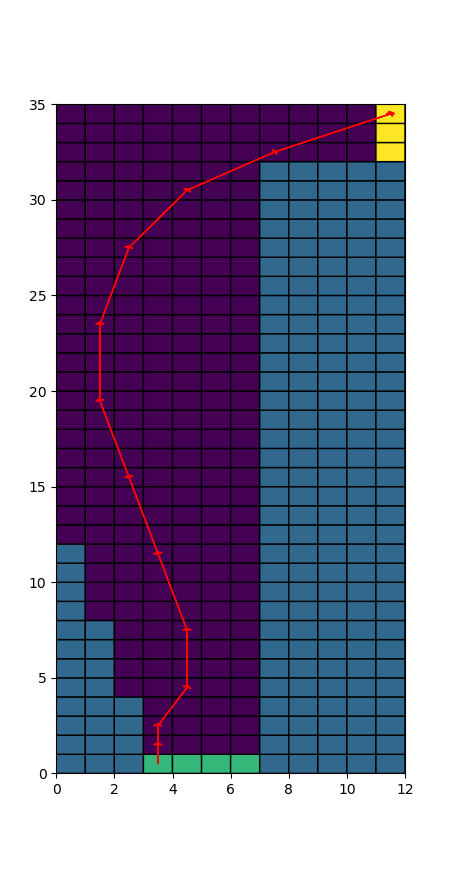
\includegraphics[width=6cm,height=6cm]{Fig/Figure_2.png}%
		\label{Fig:1:d}}
	\caption{子图包使用测试}\label{Fig:1}
\end{figure}

\section{表}
本节仅展示使用常见的三线表
\begin{lstlisting}
\begin{table}
	\caption{\label{TDF_para}涵道模型参数}	%表题在上
	\centering	% 表居中
	\small	% 表内字体小一号(即设置成和表题字号一致)
	\begin{tabular}{cccc}	% cccc表示4列并居中,若列之间需要分隔符则设置为|c|c|c|c|
		\hline	% \hline表示横线。列之间的元素用&分隔,\tabularnewline表示换行
		参数符号 & 数值 & 参数符号 & 数值 \tabularnewline 
		\hline 
		$I_x$ & $054593$ 		   & $I_y$ & $0.017045         $ \tabularnewline
		$l_1$ & $0.0808\,\text{m}$ & $l_2$ & $0.175\,\text{m}  $ \tabularnewline 
		$l_4$ & $0.2415\,\text{m}$ & $l_5$ & $0.1085\,\text{m} $ \tabularnewline
		\hline 
	\end{tabular}
\end{table}
\end{lstlisting}
\begin{table}
	\caption{\label{TDF_para}涵道模型参数}
	\centering
	\small 
	\begin{tabular}{cccc}
		\hline 
		参数符号 & 数值                & 参数符号 & 数值                 \tabularnewline
		\hline 
		$I_x$   & $054593$ 		     & $I_y$   & $0.017045         $ \tabularnewline
		$l_1$   & $0.0808\,\text{m}$ & $l_2$   & $0.175\,\text{m}  $ \tabularnewline 
		$l_4$   & $0.2415\,\text{m}$ & $l_5$   & $0.1085\,\text{m} $ \tabularnewline
		\hline 
	\end{tabular}
\end{table}

\section{公式}
除了前面讲行内公式,常用的还有行间公式。公式中的数学符号可自行百度,本章仅介绍常用的几种公式环境。

单独成行的行间公式在 \LaTeX{} 里由equation 环境包裹。equation 环境为公式自动生成一个编号,这个编号可以用\textbackslash{}label 和\textbackslash{}ref 生成交叉引用,amsmath 宏包的\textbackslash{}eqref 可为引用自动加上圆括号;如式\eqref{eq_1}所示。
\begin{lstlisting}
\begin{equation}
	a+b=c	\label{eq_1}
\end{equation}
\end{lstlisting}
\begin{equation}
	a+b=c	\label{eq_1}
\end{equation}
若不需要编号则加星号,改为
\begin{lstlisting}
\begin{equation*}
	a+b=c
\end{equation*}
\end{lstlisting}
其他环境类似。当使用 \texttt\$ 开启行内公式输入,或是使用{equation} 环境时,\LaTeX\ 就进入了数学模式。
数学模式相比于文本模式有以下特点:
\begin{enumerate}
	\item 数学模式中输入的空格被忽略。数学符号的间距默认由符号的性质(关系符号、运算符等)决定。
	需要人为引入间距时,使用 \textbackslash{}{quad} 和 \textbackslash{}{qquad} 等命令。
	\item {不允许有空行(分段)}。行间公式中也无法用 $ \verb|\\|$命令手动换行。排版多行公式需要用到 其他各种环境。
	\item 所有的字母被当作数学公式中的变量处理,字母间距与文本模式不一致,也无法生成单词之间的空格。
	如果想在数学公式中输入正体的文本,简单情况下可用 \textbackslash{}{mathrm} 命令。
	或者用 {amsmath} 提供的 \textbackslash{}{text} 命令(仅适合在公式中穿插少量文字。如果你的情况正好相反,需要在许多文字中穿插使用公式,则应该像正常的行内公式那样用,而不是滥用 \textbackslash{}{text} 命令)。
\end{enumerate}	

实际上更常用的的是多行公式,不需要对齐的公式组可以使用gather环境,需要对齐的公式组用align 环境。
长公式内可用$ \verb|\\|$ 换行。

如果需要罗列一系列公式,并令其按照等号对齐,可用align 环境,它将公式用\& 隔为两部分并对齐。分隔符通常放在等号左边:
\begin{lstlisting}
\begin{align}
	a & = b + c \\
	& = d + e
\end{align}
\end{lstlisting}
\begin{align}
a & = b + c \\
& = d + e
\end{align}
align 环境会给每行公式都编号。

如果不需要按等号对齐,只需罗列数个公式,可用gather环境:
\begin{lstlisting}
\begin{gather}
	a  = b + c \notag \\
	f = d + e 
\end{gather}
\end{lstlisting}
\begin{gather}
	a  = b + c \notag  \\
	f = d + e 
\end{gather}
gather 环境同样会给每行公式都编号,如果某行不需要编号可在行末用\textbackslash{}notag 仅去掉某行的编号。

align 和gather 有对应的不带编号的版本align* 和gather*。

另一个常见的需求是将多个公式组在一起公用一个编号,编号位于公式的居中位置。为此,
amsmath 宏包提供了诸如aligned、gathered 等环境,与equation 环境套用。以-ed 结尾的
环境用法与前一节不以-ed 结尾的环境用法一一对应。我们仅以aligned 举例:
\begin{lstlisting}
\begin{equation}
	\begin{aligned}
		a &= b + c \\
		d &= e + f + g \\
		h + i &= j + k \\
		l + m &= n
	\end{aligned}
\end{equation}
\end{lstlisting}
\begin{equation}
	\begin{aligned}
		a &= b + c \\
		d &= e + f + g \\
		h + i &= j + k \\
		l + m &= n
	\end{aligned}
\end{equation}
split 环境和aligned 环境用法类似,也用于和equation 环境套用,区别是split 只能
将每行的一个公式分两栏,aligned 允许每行多个公式多栏。

分段函数通常用amsmath 宏包提供的cases 环境,可参考文献\parencite{_c}

amsmath 宏包还直接提供了多种排版矩阵的环境,包括不带定界符的matrix,以及带各种定界符的矩阵pmatrix、bmatrix、Bmatrix、vmatrix、Vmatrix。
其中中括号版的bmatrix最常用。这些矩阵环境需要在公式中使用,比如 gather 环境。
\begin{lstlisting}
\begin{gather}
	\boldsymbol{A}= \begin{bmatrix}
		x_{11} & x_{12} & \ldots & x_{1n} \\
		x_{21} & x_{22} & \ldots & x_{2n} \\
		\vdots & \vdots & \ddots & \vdots \\
		x_{n1} & x_{n2} & \ldots & x_{nn}
	\end{bmatrix}
\end{gather}
\end{lstlisting}
\begin{gather}
\boldsymbol{A}= \begin{bmatrix}
	x_{11} & x_{12} & \ldots & x_{1n} \\
	x_{21} & x_{22} & \ldots & x_{2n} \\
	\vdots & \vdots & \ddots & \vdots \\
	x_{n1} & x_{n2} & \ldots & x_{nn}
   \end{bmatrix}
\end{gather}	
其中矩阵/向量加粗使用\textbackslash{}boldsymbol\{\}命令,bm宏包的\textbackslash{}bm\{\}命令和unicode-math包有兼容性问题,若使用unicode-math包,就不能使用bm包加粗,unicode-math的一些加粗命令比较特别(具体在math\_font文件夹的测试文件对比差异)。若不使用unicode-math,boldsymbol命令也没法加粗,则再考虑借助bm包。简而言之,公式加粗使用\textbackslash{}boldsymbol\{\}命令。另外还可以使用array环境排版矩阵,类似tabular环境,用$ \verb|\\|$ 和\& 用来分隔行和列,这里不再赘述。	
\begin{lstlisting}
\begin{array }[外部对齐tcb]{列对齐lcr}
	行列内容
\end{array}
\end{lstlisting}

另外注意排版分式时,有两种方法:\textbackslash{}frac或者\textbackslash{}dfrac,效果分别为$ \frac{1}{2} $和$ \dfrac{1}{2} $。以上介绍的数学环境中,空格可参考文献\parencite{_c},例如常用\textbackslash{}quad。

需要局部更改字号时,可以使用tutorial文件夹lshort-zh-cn.pdf的5.1节进行更改,如加\textbackslash{}small使得字号小一号。
\section{定理}
在gxuthesis.cls文件的最后,已经用\textbackslash{}newtheorem命令定义了几种定理环境,包括:定义、假设、定理、结论、引理、公理、推论、性质等等,统称定理环境,关于\textbackslash{}newtheorem的用法,可参考\cite{_g,_c}或自行百度。要下面提供几个例子,在横线之间的深色区域是代码,效果在相应下方表示:
\begin{lstlisting}
\begin{assumption}
	加权矩阵${{\boldsymbol{W}}_{1}}$和 ${{\boldsymbol{W}}_{2}}$ 是对称矩阵,且$ {{\boldsymbol{W}}_{2}}$非奇异。	\label{assum_dca1}
\end{assumption}
\end{lstlisting}
\begin{assumption}
	加权矩阵${{\boldsymbol{W}}_{1}}$和 ${{\boldsymbol{W}}_{2}}$ 是对称矩阵,且$ {{\boldsymbol{W}}_{2}}$非奇异。	\label{assum_dca1}
\end{assumption}

定理用法和假设类似:
\begin{lstlisting}
\begin{theorem}
	如果假设\ref{assum_dca1}成立,$\boldsymbol{F}$满足式\eqref{eq_F}的定义,且${{\boldsymbol{W}}_{1}}$非奇异,则有$0\le e \left( \boldsymbol{F} \right) < 1$,其中$e \left( \boldsymbol{F} \right)$是 $\boldsymbol{F}$的特征值。	\label{the_dca2}
\end{theorem}
\end{lstlisting}
\begin{theorem}
	如果假设\ref{assum_dca1}成立,$\boldsymbol{F}$满足上式的定义,且${{\boldsymbol{W}}_{1}}$非奇异,则有$0\le e \left( \boldsymbol{F} \right) < 1$,其中$e \left( \boldsymbol{F} \right)$是 $\boldsymbol{F}$的特征值。	\label{the_dca2}
\end{theorem}
\begin{remark}
	定理环境的编号可自定义,但通常不需要再进行设置,因为模板文件gxuthesis.cls文件已经定义好。
\end{remark}

---------------------------------------------------------

2022年5月更新:

根据最新的博士论文送审结果,定理等环境统一把原来的斜体改成正体。在此引用一下参考文献\cite{_g}的内容:

amsthm 提供了 \textbackslash{}theoremstyle 命令支持定理格式的切换,在用 \textbackslash{}newtheorem 命令定义定 理环境之前使用。amsthm 预定义了三种格式用于 \textbackslash{}theoremstyle:plain 和 LATEX 原始的格式 一致;definition 使用粗体标签、正体内容;remark 使用斜体标签、正体内容。

以上部分在gxuthesis.cls文件最后一部分设置。

---------------------------------------------------------

amsthm 还提供了一个 proof 环境用于排版定理的证明过程。proof 环境末尾自动加上一个证毕符号:
\begin{proof}
	显然有
	\begin{equation*}
	E=mc^2
	\end{equation*}
	证毕
\end{proof}

proof的大更多用法见参考文献\cite{_g}。gxuthesis.cls文件的最后,跟所有定理环境一样,只是把英文”Proof“改成中文“证明”。

\section{参考文献}

再次强调,使用其他参考文献管理软件的用户以及不使用任何软件的“裸奔”的用户不需要关注任何关于zetero的东西。
\begin{lstlisting}
	关于参考文献这块,很多同学有疑问。只有记住一点:不管用什么参考文献管理工具,最终目的是生成一个bib文件,bib文件里是特定格式的文献信息。bib文件当作文本打开,里面就是文献的元数据。
\end{lstlisting}

通常学位论文参考文献是基于BibTeX进行的,本模板使用的是BibLaTeX,或者叫Biber。关于这部分知识可参考文献\parencite{_c,_g}的第六章,6.1节参考文献和BIBTEX工具。所以使用TeXstudio或者vscode的时候需要注意调整正确的参数进行编译。

引用前手动加空格,如:

引用前没有加空格\parencite{_c,_g}的第六章,引用后面有空格。

引用前手动加空格 \parencite{_c,_g}的第六章,引用后面有空格。

手写方括号 [6]。引用后面没空格。

生成方括号 \parencite{_k}。引用后面没空格。


参考文献引用和著录是基于ZOTERO这个软件进行的。视频教程见\parencite{_k}。此外,为了符合毕业论文撰写规范,需设置参数。按照视频教程安装完必要的插件(如Better BibTeX)后,在编辑->首选项进行设置。图\ref{op1}到图\ref{op11}所示的是我的zotero软件设置。其中最重要的是\ref{op10}的设置要排除的选项,多余的显示会让审稿人反感,按照论文撰写规范进行即可。在毕业论文撰写时,在编辑->首选项->Better BibLTeX->Fields中,Fields to omit from export填month,abstract,note,extra,file,keywords,type,url,doi,就是在参考文献著录中排除这些多余的项,避免过于复杂。而在写本模板使用说明时,没有排除url,因为很多参考资料是网页。

\begin{lstlisting}
    使用zotero,有时候科学上网很重要。
\end{lstlisting}

在zotero软件点击文件->导出文献库,如图\ref{output}所示,再在导出对话框图\ref{output_format}选择导出格式为Better BibLaTeX,同时勾选Keep updated选项保持自动更新,再点击ok,在弹出的对话框图\ref{output_name}确定保存路径和文件名,例如我的是MyLibrary.bib,这也是我整个读书生涯的文献库bib文件。如果写小论文的话通常导出格式是BibTeX或者Better BibTeX(这里按照期刊的要求来即可,文献管理软件的好处就是快速自动生成一个文件库)。关于BibTeX和BibLaTeX的区别这里不做展开。

得到文献库后,在gxuthesis.tex文件第九行使用\textbackslash{}addbibresource命令,添加文献库。引用某文献时秩序在zotero选中某文献条目,然后按Ctrl+Shift+C,复制引用关键字(Citation Key)到剪切板(快捷键可自定义)。然后在tex文件编辑界面直接粘贴,默认的时上标形式,若需要非上标形式,可以改为\textbackslash{}parencite\{xxx\},其中xxx是Citation Key。这里的操作和认为设置的首选项参数有关,需要在编辑->首选项->导出界面的默认格式一栏选中相应的项,同时在编辑->首选项->高级->快捷键设置为默认值。

---------------------------------------------------------------------------------

2020年12月2日测试:
下载最新zotero,从知网和谷歌捕获文献(刚打开网页最好稍等一会再点击插件,谷歌可能需要现人机验证),对文献\parencite{Renduchintala_2019}、\parencite{milz2020design}进行引用。

---------------------------------------------------------------------------------

---------------------------------------------------------------------------------

2021年9月14日测试:
使用endnote的用户也可以利用导出的bib文件生成参考文献著录信息,导出选项是bibTeX,貌似没有更多导出设置选项。导出设置没有zotero那么灵活丰富,得到bib文件后要引用某论文需要自行查找标签(label,也有软件叫引用关键字Citation Key)\{xxx\}然后手打\textbackslash{}cite\{xxx\}。欢迎熟悉endnote的同学来信告诉我更好的办法。

---------------------------------------------------------------------------------

2023年3月8日测试:参考文献管理软件经常更新,但还是那句话,无论什么工具,最终得到bib文件即可,在期刊的文章页或者谷歌学术搜索页,只需要复制/下载bibtex的内容。得到这些元数据后甚至自己往bib文件里加都可以。

---------------------------------------------------------------------------------

2023年11月测试。论文写完记得断掉bib文件自动更新,在zotero的插件Better BibTeX自动导出设置里删除不希望再继续同步到项。否则更改软件中的文献后,论文的bib文件也同步更改,但有时候这不是想要的。
\begin{lstlisting}
    另外有同学反映,换了电脑后重新导出的bib文件Citation Key值不同,记得设置好Better BibTeX之后,在著录条目界面全选著录(或仅选想更新的著录)然后右键选Better BibTeX更新refresh一下。然后在Automatic export选项点击Export now立即更新bib文件(按理说勾选了自动更新选项他会自动更新,但为了确保万无一失还是点一下)。
\end{lstlisting}
\begin{figure}
	\centering
	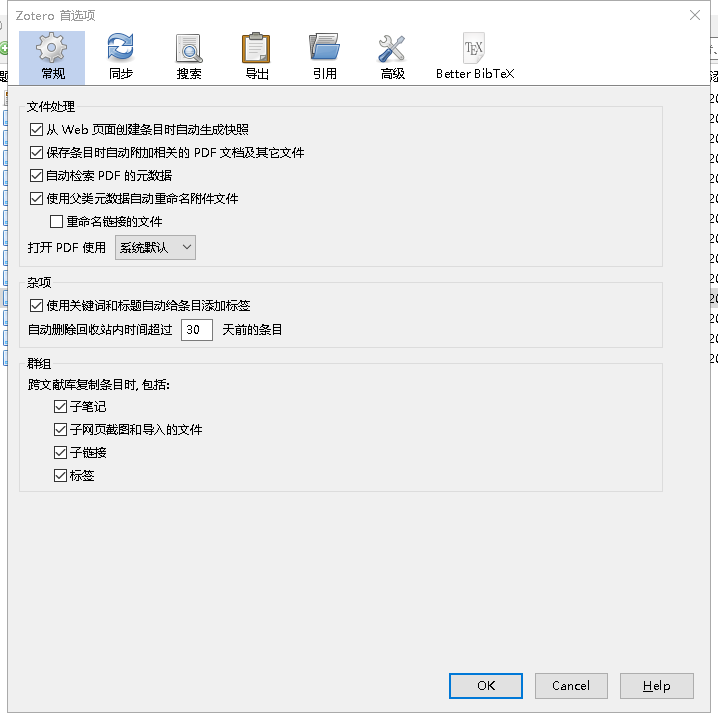
\includegraphics[scale=0.8]{Fig/zotero1.png}
	\caption{\label{op1}常规}
\end{figure}
\begin{figure}
	\centering
	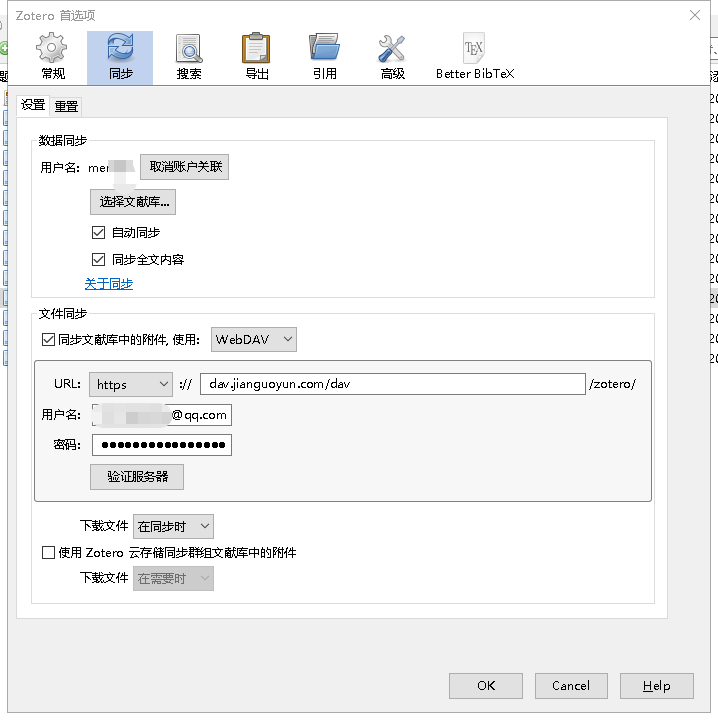
\includegraphics[scale=0.8]{Fig/zotero2.png}
	\caption{\label{op2}同步1}
\end{figure}
\begin{figure}
	\centering
	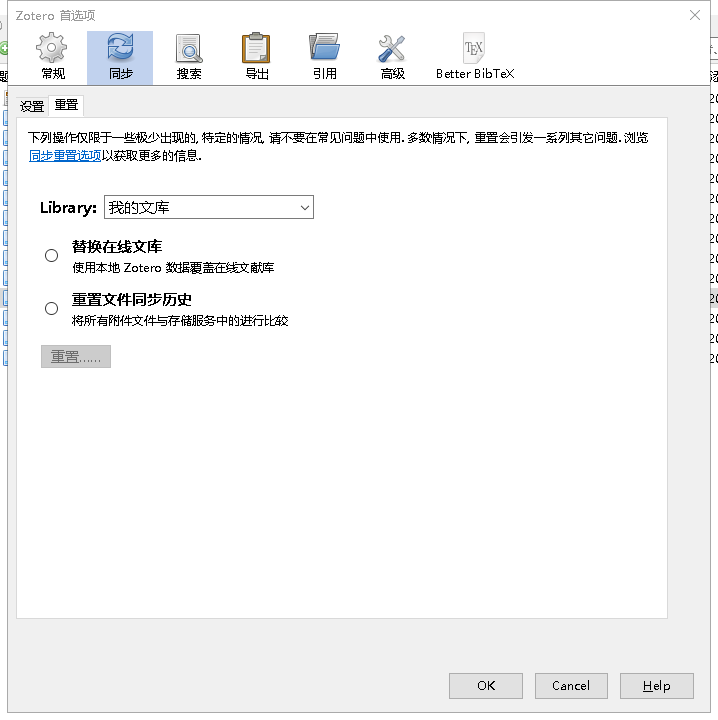
\includegraphics[scale=0.8]{Fig/zotero3.png}
	\caption{\label{op3}同步2}
\end{figure}
\begin{figure}
	\centering
	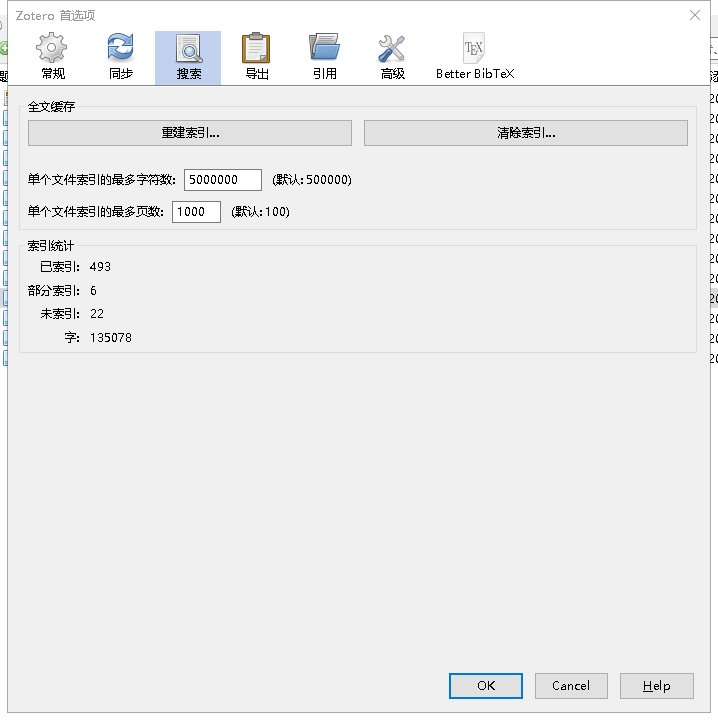
\includegraphics[scale=0.8]{Fig/zotero4.png}
	\caption{\label{op4}搜索}
\end{figure}
\begin{figure}
	\centering
	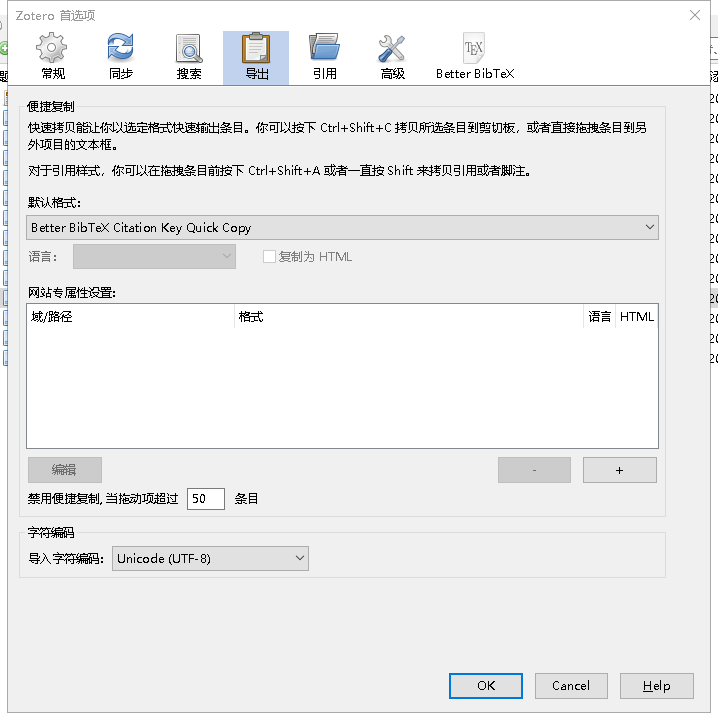
\includegraphics[scale=0.8]{Fig/zotero5.png}
	\caption{\label{op5}导出}
\end{figure}
\begin{figure}
	\centering
	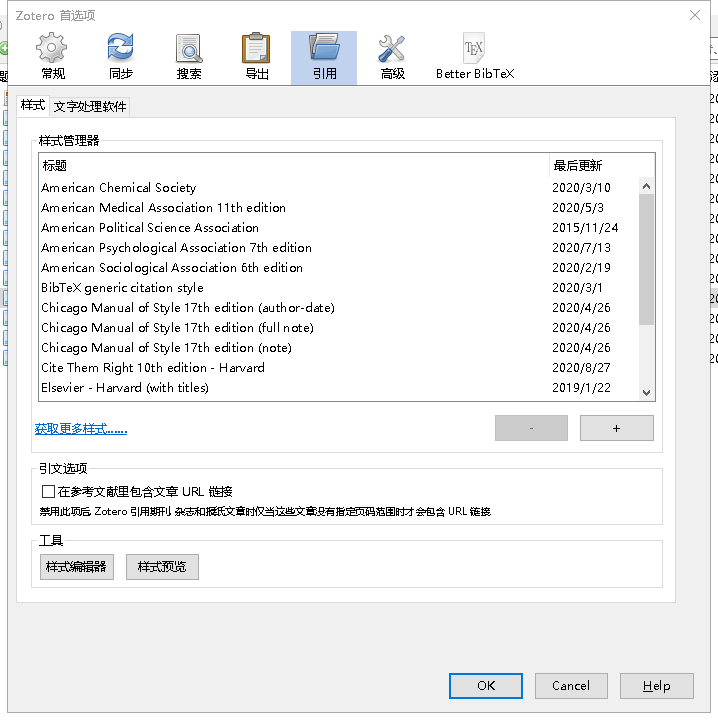
\includegraphics[scale=0.8]{Fig/zotero6.png}
	\caption{\label{op6}引用}
\end{figure}
\begin{figure}
	\centering
	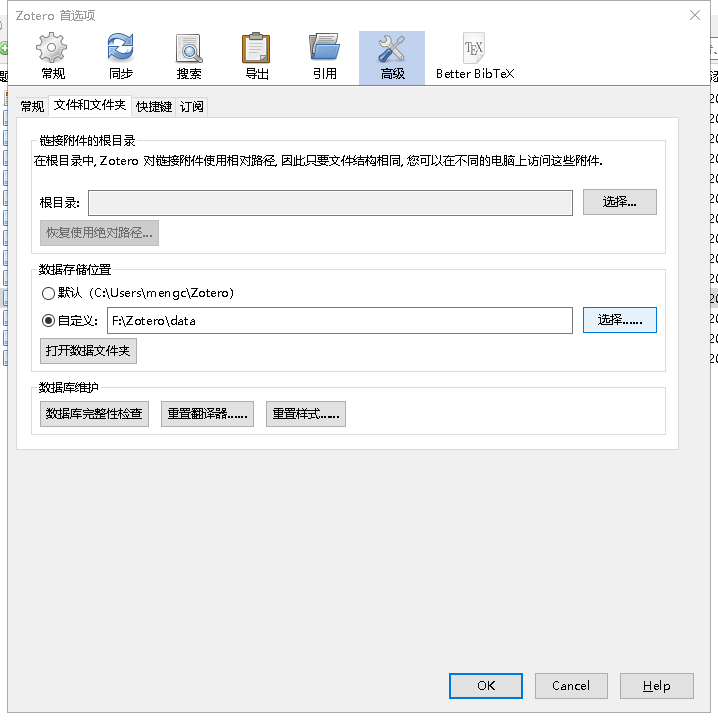
\includegraphics[scale=0.8]{Fig/zotero7.png}
	\caption{\label{op7}高级1}
\end{figure}
\begin{figure}
	\centering
	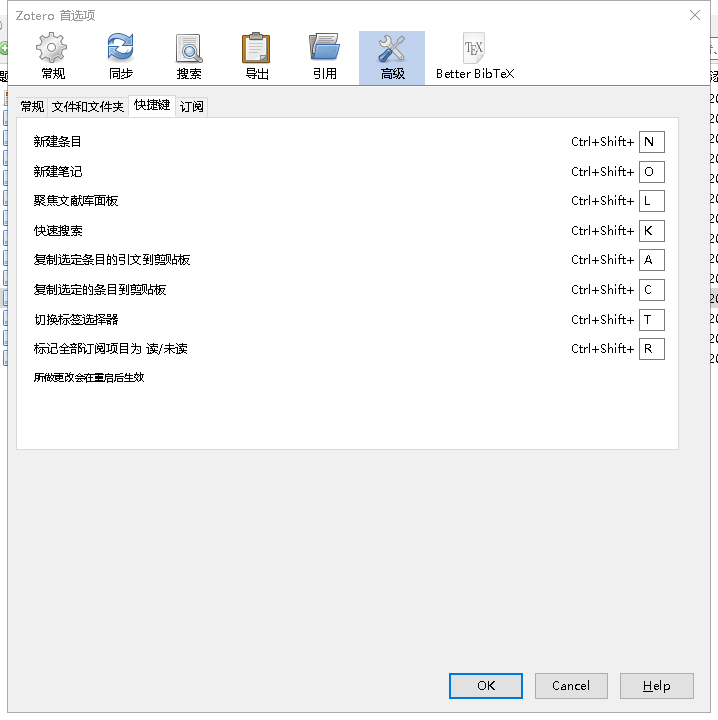
\includegraphics[scale=0.8]{Fig/zotero8.png}
	\caption{\label{op8}高级2}
\end{figure}
\begin{figure}
	\centering
	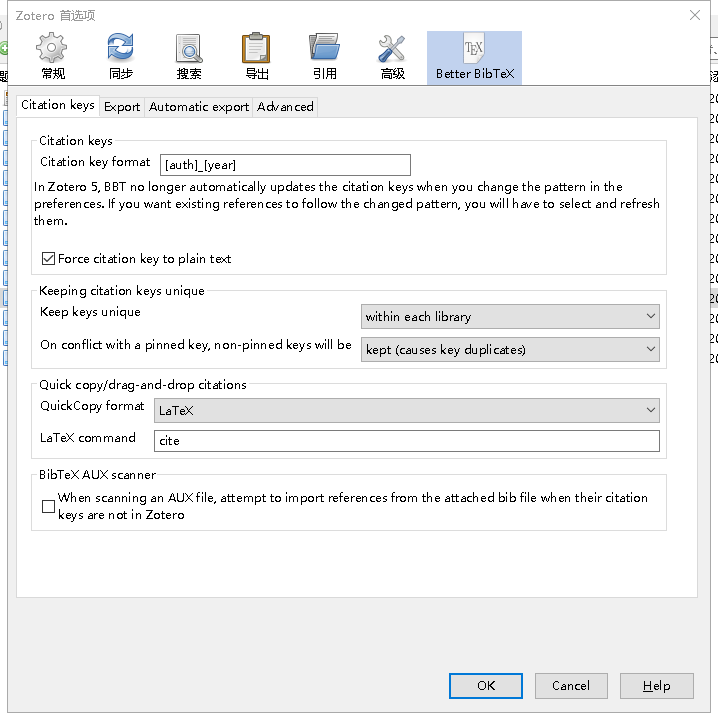
\includegraphics[scale=0.8]{Fig/zotero9.png}
	\caption{\label{op9}Better BibTeX1}
\end{figure}
\begin{figure}
	\centering
	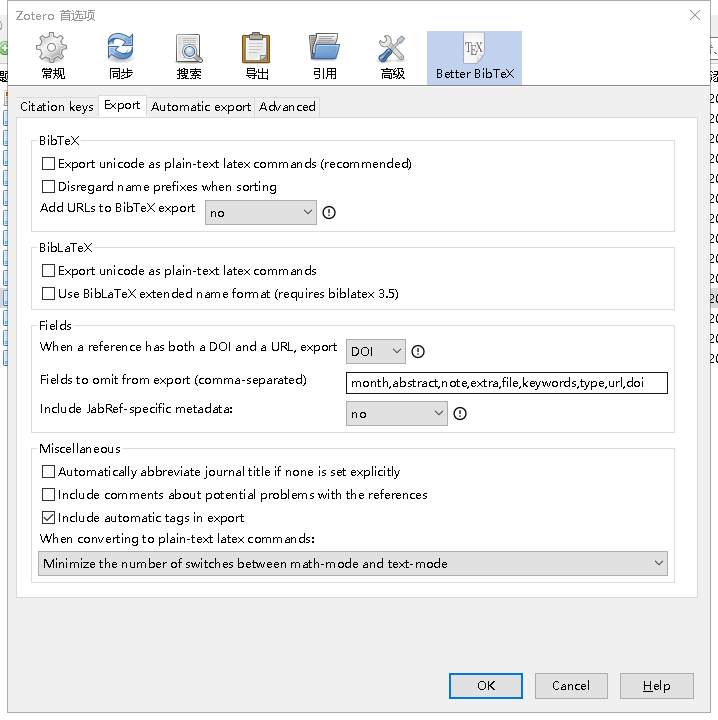
\includegraphics[scale=0.8]{Fig/zotero10.png}
	\caption{\label{op10}Better BibTeX2}
\end{figure}
\begin{figure}
	\centering
	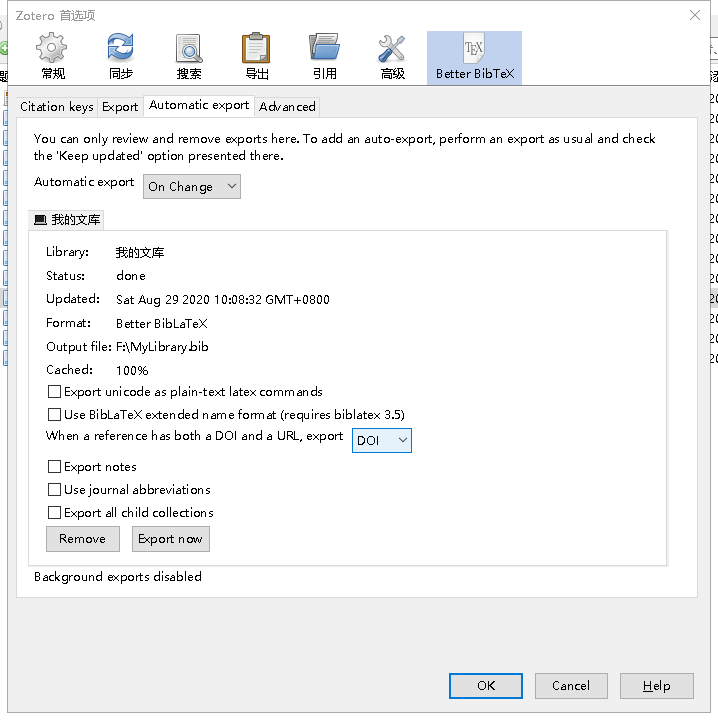
\includegraphics[scale=0.8]{Fig/zotero11.png}
	\caption{\label{op11}Better BibTeX3}
\end{figure}

\begin{figure}[htbp]
	\centering
	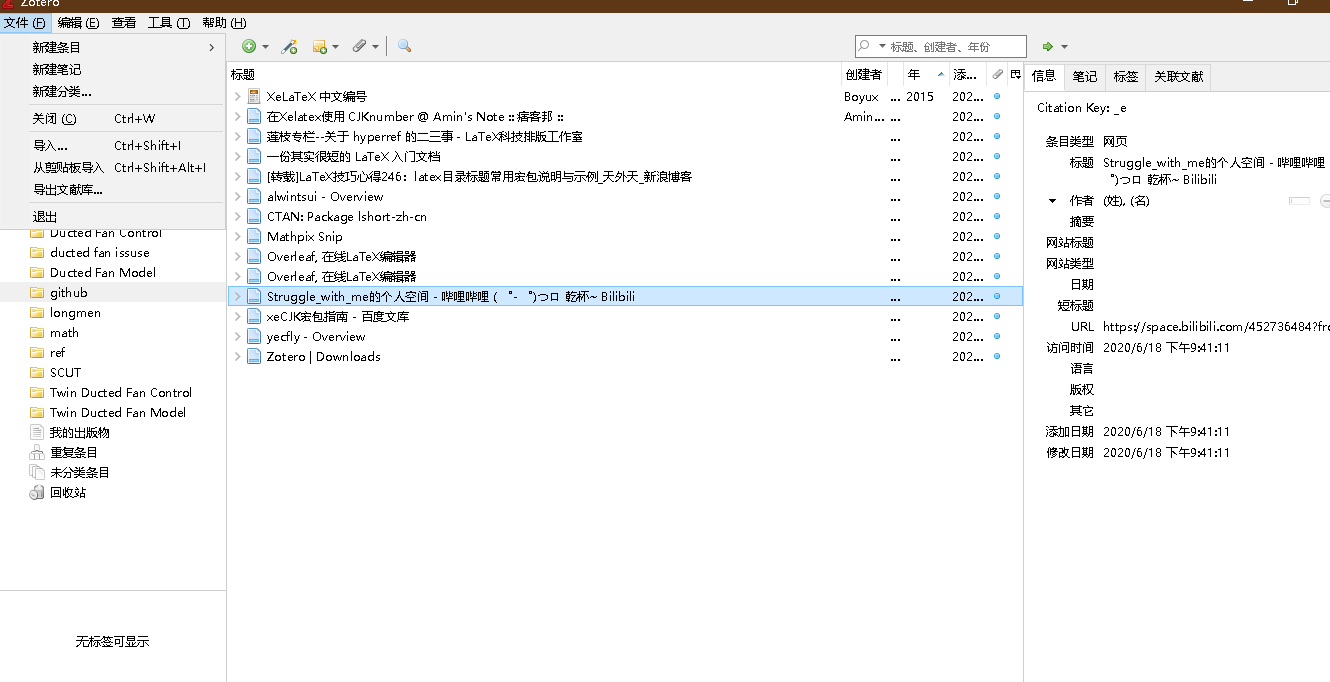
\includegraphics[scale=0.42]{Fig/zotero12.png}
	\caption{\label{output}导出文献库}
\end{figure}

\begin{figure}[htbp]
	\centering
	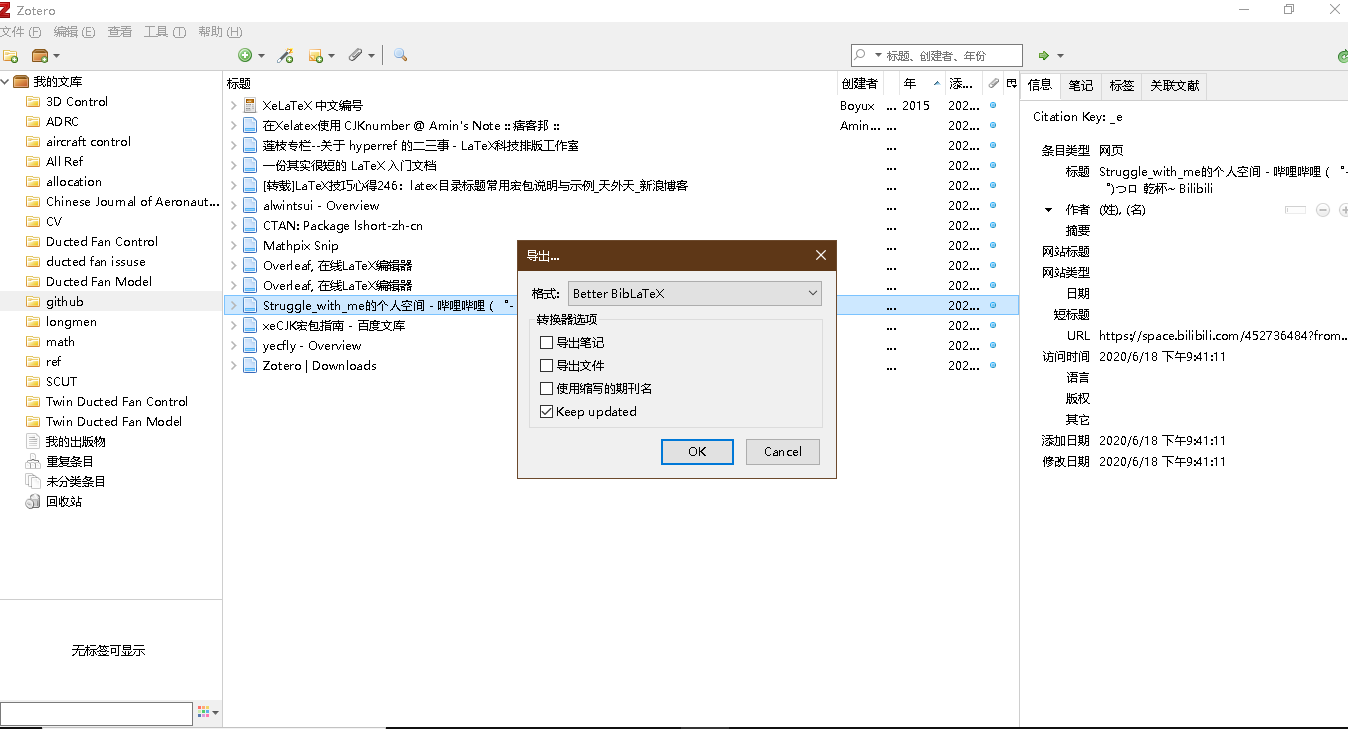
\includegraphics[scale=0.42]{Fig/zotero13.png}
	\caption{\label{output_format}导出格式}
\end{figure}

\begin{figure}[htbp]
	\centering
	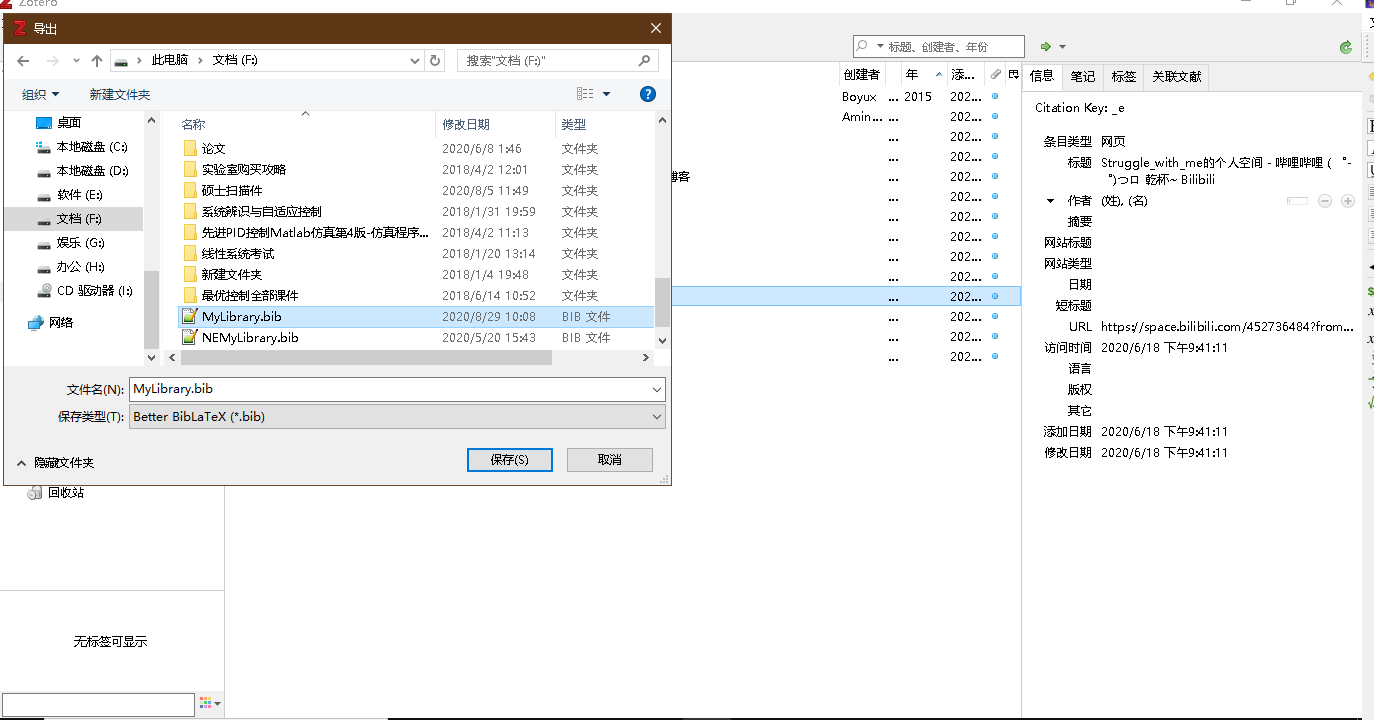
\includegraphics[scale=0.42]{Fig/zotero14.png}
	\caption{\label{output_name}导出文件名}
\end{figure}









 % 第三章
% 自行根据需要添加章节。
...
\chapter{结\texorpdfstring{\quad}{}论}
本文主要是展示如何使用修改“祖传模板”得到的新模板,在使用时直接替换成自己的论文内容即可。

本模板难免有不足之处,主要是我本人的论文涉及的格式有限,有些地方没探索到自然就没去设置。比如附录,附录的图文并茂等等,我本人是没有研究的,这里仅仅做了一些初步的工作,不过对很多同学来说本模板是够用的。希望有能帮助到华工的同学们,有不足之处请多多理解,可以通过邮件联系我,我会尽量回复。
 % 结论
...
\printbibliography	% 参考文献著录
%%%%%%%%%%%%%%%%%%%此部分为附录环境代码,是比较笨的方法来适应论文撰写规范%%%%%%%%%%%%%%%%%%%%%%%%%%%%%%%%%%%%%%
%对只有一个附录,标题不编号比较美观。
%%%%%%%%%%%%%%%%%%%%%%%%%%%%%%%%%%%%%%%%%%%%%%%%%%%%%%%%%%%%%%%%%%%%%%%%%%%%%%%%%%%%%%%%%%%%%%%%%%%%%%%%%%%%
\setcounter{chapter}{1} %从1开始编号
\setcounter{section}{0}
\setcounter{equation}{0}
\setcounter{table}{0}   
\setcounter{figure}{0}
\chapter{附\texorpdfstring{\quad}{}录} %附录
%%%%%%%%%%%%%%%%%%%%%%%%%%%%%%%%%%%%%%%%%%%%%%%%%%%%%%%%%%%%%%%%%%%%%%%%%%%%%%%%%%%%%%%%%%%%%%%%%%%%%%%%
%%%%%%%%%%%%以下为用户代码,用于撰写您的论文%%%%%%%%%%%%%%%%%%%%%%%%%%%%%%%%%%%%%%%%%%%%%%%%%%%%%%%%%%%%%%


在论文撰写规范中,下面两段话让人费解:

\begin{enumerate}
	\item 	对需要收录于学位论文中但又不适合书写于正文中的附加数据、方案、资料、详细公式推导、计算机程序、统计表、注释等有特色的内容,可做为附录排写,序号采用“附录1”、“附录2”等。	
	\item	公式序号按章编排,如第一章第一个公式序号为“(1-1)”,附录2中的第一个公式为“(2-1)”等。
\end{enumerate}

论文撰写规范要求的附录和通常书籍上使用附录A、附录B等编号的不一样,容易和正文混淆。特殊的要求和代码的耦合,使我不得不使用比较笨的方法来设计附录部分的模板。

\section{测试测试测试}
\subsection{测试测试测试}
%
测试测试测试测试测试测试测试测试测试测试测试测试测试测试测试测试测试测试测试测试测试测试测试测试测试测试测试测试测试测试测试测试测试测试测试测试测试测试测试测试测试测试测试测试测试测试测试测试测试测试测试测试测试测试测试测试测试测试测试测试测试测试测试测试测试测试测试测试测试测试测试测试测试测试测试测试测试测试测试测试测试测试测试测试测试测试测试测试测试测试测试测试测试测试测试测试测试测试测试测试测试测试测试测试测试测试测试测试测试测试测试测试测试测试测试测试测试测试测试测试测试测试测试测试测试测试测试测试测试测试测试测试测试测试测试测试测试测试测试测试测试测试测试测试测试测试测试测试测试测试测试测试测试
\begin{align}
\left\{\begin{array}{l}
\dot{v}_{1}(t)=v_{2}(t) \\
\dot{v}_{2}(t)=R^{2}\left(-\zeta_{1}\left[v_{1}(t)-v_c(t)\right]^{\alpha}-\zeta_{2}\left[\dfrac{v_{2}(t)}{R}\right]^{\beta}\right)
\end{array}\right.	
\end{align}

\begin{align}
\left\{\begin{array}{l}
\dot{v}_{1}(t)=v_{2}(t) \\
\dot{v}_{2}(t)=R^{2}\left(-\zeta_{1}\left[v_{1}(t)-v_c(t)\right]^{\alpha}-\zeta_{2}\left[\dfrac{v_{2}(t)}{R}\right]^{\beta}\right)
\end{array}\right.	
\end{align}
\begin{figure}[htbp]
	\centering	
	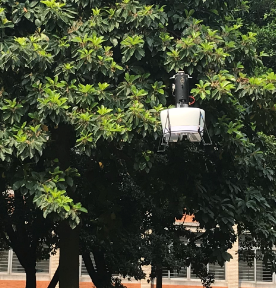
\includegraphics[scale=1]{Fig/DFUAV_f31.png}
	\caption{\label{fig_case1}测试测试测试}
\end{figure}
\begin{figure}[htbp]
	\centering	
	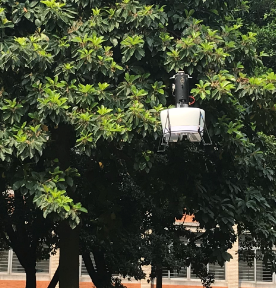
\includegraphics[scale=1]{Fig/DFUAV_f31.png}
	\caption{\label{fig_case2}测试测试测试}
\end{figure}
\begin{table}
	\caption{\label{DF_para1}测试测试测试}
	\centering{}%
	\small 
	\begin{tabular}{cccccc}
		\hline 
		参数符号 & 数值&参数符号 & 数值&参数符号 & 数值\tabularnewline
		\hline 
		$ A_x,A_y,A_z $  & $ 0.04082\,\text{m}^2 $ &$ \rho $        &$1.225\,\text{kg}/\text{m}^3$&$ I_b $           & $ 0.000029 $               \tabularnewline
		$ k_{\varpi} $   & $1.13342 \times 10^{-6}$& $ d_{\varpi} $ & $1.13342 \times 10^{-7}$ 	  &$k_{\delta} $     & $ 0.01495 $ 			      \tabularnewline
		$C_{D,x},C_{D,y}$& $ 0.43213 $             &$ C_{D,z} $     & $ 0.13421 $             	  &	$ q_a $ 	     & $ 1.49 $ 				  \tabularnewline
		$ l_{a} $        & $ -0.1121\,\text{m} $   & $ d_{ds} $     & $ 0.01495 $			  	  &$ d_{af} $        & $ 0.01495 $    			  \tabularnewline
		$ R $            & $ 0.11\,\text{m} $      &$ b $           & $ 2 $       			   	  &$ S $ 			 & $ 0.04082\,\text{m}^2 $    \tabularnewline
		$C_{l_{\alpha}}$ & $ 2.212\,/\text{rad} $  &$C_{l, \max } $ & $ 1.05 $ 				   	  &$ C_{l, \min } $  & $ -1.05 $ 				  \tabularnewline
		$ l_2 $          & $ 0.06647\,\text{m} $   &$ l_1 $         & $ 0.17078\,\text{m} $    	  &	$ m $ 		     & $ 1.53\,\text{kg} $ 		  \tabularnewline
		$ C_{d, o } $    & $ 0.9 $                 &$ C_{d, g } $   & $ 0.9 $					  &$ C_{duct} $      & $ 0.78497 $	 			  \tabularnewline
		$ I_x $          & $ 0.02548 $ 			   &$ I_y $         & $ 0.02550 $                 &$ I_z $			 & $ 0.00562 $ 				  \tabularnewline
		\hline 
	\end{tabular}	
\end{table}

\begin{table}
	\caption{\label{TDF_para2}测试测试测试}
	\centering{}%
	\small 
	%	\resizebox{\textwidth}{!}{
	\begin{tabular}{cccccc}
		\hline 
		参数符号 & 数值&参数符号 & 数值&参数符号 & 数值\tabularnewline
		\hline 
		$ I_x $ & $ 054593 $ &$ I_y $ & $ 0.017045 $& $ I_z$ & $ 0.049226 $ \tabularnewline
		$ l_{1} $ & $ 0.0808\,\text{m} $&$ l_{2} $ & $ 0.175\,\text{m} $ &$ l_3 $ & $ 0.06647\,\text{m} $ \tabularnewline 
		$ l_4 $ & $ 0.2415\,\text{m} $ &$ l_5 $ & $ 0.1085\,\text{m} $& $ m $ & $ 3.7\,\text{kg} $ \tabularnewline
		\hline 
	\end{tabular}	%}
\end{table}

\section{测试测试测试}
\subsection{测试测试测试}
%
测试测试测试测试测试测试测试测试测试测试测试测试测试测试测试测试测试测试测试测试测试测试测试测试测试测试测试测试测试测试测试测试测试测试测试测试测试测试测试测试测试测试测试测试测试测试测试测试测试测试测试测试测试测试测试测试测试测试测试测试测试测试测试测试测试测试测试测试测试测试测试测试测试测试测试测试测试测试测试测试测试测试测试测试测试测试测试测试测试测试测试测试测试测试测试测试测试测试测试测试测试测试


 % 附录
\chapter{攻读学位期间发表论文与研究成果清单} % 
\pubfont %  


\begin{enumerate}[topsep = 0 pt, itemsep= 0 pt, parsep=0pt, partopsep=0pt, leftmargin=44pt, itemindent=0pt, labelsep=6pt, label=(\arabic*)]
	\item 论文1:
	\item 
 


\end{enumerate}

\normalsize % \normalsize可以将下文调回和正文一样的字号,这个随个人喜好。注释掉的话,致谢就就跟随《攻读博士/硕士学位期间取得的研究成果》的字号。 % 成果
\chapter{致\texorpdfstring{\quad}{}谢}
%把下面文字替换
\begin{center}
这次你离开了没有像以前那样说再见,再见也他妈的只是再见 
~\\
我们之间从来没有想象的那么接近,只是两棵树的距离 
~\\
你是否还记得山阴路我八楼的房间,房间里唱歌的日日夜夜 
~\\
那么热的夏天你看着外面,看着你在消逝的容颜 
~\\
我多么想念你走在我身边的样子,想起来我的爱就不能停止 
~\\
南京的雨不停地下不停地下,就像你沉默的委屈 
~\\
一转眼,我们的城市又到了夏天,对面走来的人都眯着眼 
~\\
人们不敢说话不敢停下脚步,因为心动常常带来危险 
~\\
我多么想念你走在我身边的样子,想起来我的爱就不能停止 
~\\
南京的雨不停地下不停地下,有些人却注定要相遇 
~\\
你是一片光荣的叶子,落在我卑贱的心 
~\\
像往常一样我为自己生气并且歌唱 
~\\
那么乏力,爱也吹不动的叶子 
\end{center}
%把上面文字替换

~\\

\begin{minipage}[t]{0.945\textwidth}%
	\begin{flushright}
		作者姓名\\
%		\today\\	% 自动时间
		2020年7月10日\\	%固定时间
		于华南理工大学
		\par\end{flushright}
\end{minipage}

 % 致谢
\end{lstlisting}
其中$\%$之后的内容为注释,...表示省略其他代码,仅保留论文内容主体部分。\textbackslash{}include\{xxx\}指令用于包含xxx.tex文件的内容,各章节的内容主要在xxx.tex中保存。在\textbackslash{}documentclass 和\textbackslash{}begin\{document\} 之间的位置称为导言区。在导言区中一般会使用\textbackslash{}usepackage 调用宏包,以及会进行对文档的全局设置。本模板的导言区除调用所需的宏包外,还进行了页眉页脚的设置。有的模板会把所有调用宏包的指令放到一个.sty宏包文件中,页面的设置放在文档类文件.cls文件中。因本人时间有限,就不做整理,欢迎有志之士加入完善。使用本模板并不需要了解导言区的指令,在需要时额外添加即可(要注意宏包冲突)。特别地,\textbackslash{}includeonly\{xxx\}指令用于使文档仅编译xxx.tex文件的内容,这就是分章节包含(include)的好处,可大大减少编译时间。

将封面打印保存为 thesis\_cover.pdf 文件,硕士使用master\_cover.docx ,博士使用 doctor\_cover.doc 。如果有更新版本的封面,可自行替换。文档类默认是博士论文,下面指令将控制添加封面与否:
\begin{lstlisting}
\documentclass[unicode,master,pdfcover]{gxuthesis}	% 使用pdf文件封面的 硕士模板
\documentclass[unicode,master]{gxuthesis}	% 不使用pdf文件封面的 硕士模板
\documentclass[unicode,pdfcover]{gxuthesis}	% 使用pdf文件封面的博士模板
\documentclass[unicode]{gxuthesis}	% 不使用pdf文件封面的博士模板
\end{lstlisting}
不使用thesis\_cover.pdf 文件指定的封面时,将使用草稿封面。草稿封面也可以减少编译时间,因此可以在最终提交论文时再使用论文封面。草稿封面用以下指令设置:
\begin{lstlisting}
%%%%%%%%%%%%%草稿封面设置%%%%%%%%%%%%%	
\title{LaTeX模板}	
\author{作者姓名}	
\supervisor{指导教师:xxx\ 教授}	
\institute{华南理工大学}	
\date{2020年5月20日}
%%%%%%%%%%%%%%%%%%%%%%%%%%%%%%%%%%%%%
\end{lstlisting}
\section{章节文件}
chapter文件夹的章节文件如chapter0x.tex等,其内容由\textbackslash{}chapter\{章名\}开头。新建一章可新建一个文件并由\textbackslash{}chapter\{新建章名\}开头填写内容即可。节及小节分别用\textbackslash{}section\{新建节名\}、\textbackslash{}subsection\{新建小节名\}命令。

正文的的书写和txt文本文件的书写类似。\LaTeX{} 源代码中,空格键和Tab键输入的空白字符视为“空格”。连续的若干个空白字符视为一个空格。一行开头的空格忽略不计。行末的回车视为一个空格;但连续两个回车,也就是空行,会将文字分段。多个空行被视为一个空行。也可以在行末使用\textbackslash{}par 命令分段。在本模板中,英文之间的空格被保留,中文之间的空格被忽略。特别地,摘要,附录,结论等两个字的大纲级别为章的章名,中间使用空格隔开。对此论文撰写规范并没有明文要求,只是为了美观。也可以全部不加空格。一般情况下,在文本文字中添加空格使用\textbackslash{}quad命令,但由于文献\parencite{_d}所述原因,直接使用\textbackslash{}quad命令会报警,因而使用\textbackslash{}texorpdfstring\{\textbackslash{}quad\}\{\},其中最后一个\{\}里面可以加一个空格,不影响使用。目录二字之间添加空格在gxuthesis.cls文件317行设置。

正文本环境中使用公式,即行内公式,需要用两个\$包围,如源码:\$a+b=c\$ 显示为$a+b=c$。使用其他字符可自行百度或阅读参考文献。再次提醒,使用\LaTeX{}撰写论文不需要研究其原理,在达到某种效果(图文显示、公式显示效果)时百度或查书寻找其代码即可。

综上,论文撰写只需要将自己的文本(包含行内公式)放到相应的章节处,并添加行间公式、图表环境并填写图表即可。行间公式、图表将在下一章介绍。

 % 第二章

\chapter{常用环境及参考文献设置}
强烈建议在使用公式、表格、定理环境时进行百度,没必要研究各种用法,只需要知道自己需要什么。因本人的论文所用表格较少,因而对表格不是很熟悉,本章对表格的介绍相应的较少。本章仅介绍本人在论文撰写过程中常用的环境以及参考文献设置。

\section{图}
图的导入需要提前准备好图片文件,最好是.png、.eps、.pdf或.jpg文件。另外,如果是从matlab导出图片文件,可使用print函数或手动导出,print函数的使用可参考ICGNC2020plot.m以及PlotToFileColorPDF.m文件等。手动导出(matlab的figure界面的“文件”->“导出设置”设置好大小、分辨率和线宽等然后点击“应用于图窗”)主要用于观察效果,可设置某种样式名称后保存该样式,下次使用时加载,具体可百度“matlab导出高清图片”。需要特别注意的是一定要1:1导入matlab生成的图片,并且图中文字设置好字体字号。否则缩放之后,图片的字号就变了,盲审老师一眼就能看出来字号不对,就很麻烦。这就是为什么要在matlab点击“应用于图窗“进行预览,观测效果后再1:1使用图片。

使用如下代码放置独立成行的图片,效果如图\ref{one_DFUAV}所示
\begin{lstlisting}
\begin{figure}[htbp]
	% 图片居中(列居中对齐)
	\centering	
	% 包含当前路径下的Fig文件夹的图片文件DFUAV_f31.png
	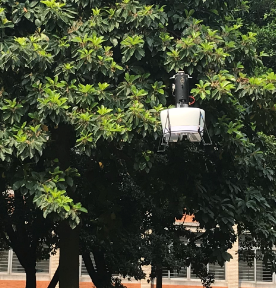
\includegraphics[scale=1]{Fig/DFUAV_f31.png} 
	% 添加标签one_DFUAV以及图标题“涵道风扇式无人机”,引用某图时使用\ref{xxx},其中xxx就是标签,图编号是自动生成的。
	\caption{\label{one_DFUAV}涵道风扇式无人机} 
\end{figure}
\end{lstlisting}
其中figure为环境名,[htbp]表示将图片设置为浮动体,实际上这在.cls文件已经设置过,因而可以省略。[scale=1]表示安装1:1的比例导入图片,还可以按其他方式导入,需要时可自行百度。
\begin{figure}[htbp]
	\centering
	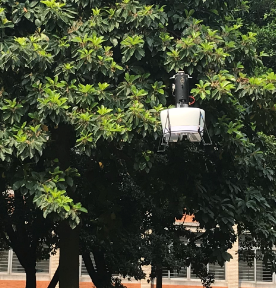
\includegraphics[scale=1]{Fig/DFUAV_f31.png}
	\caption{\label{one_DFUAV}涵道风扇式无人机}
\end{figure}

使用如下代码划分页面并排放置图\ref{Hawk}、图\ref{GTSpy}
\begin{lstlisting}
\begin{figure}[htbp]
	\centering
	\begin{minipage}[c]{0.5\textwidth} % minipage将页面划分为0.5\textwidth
		\centering
		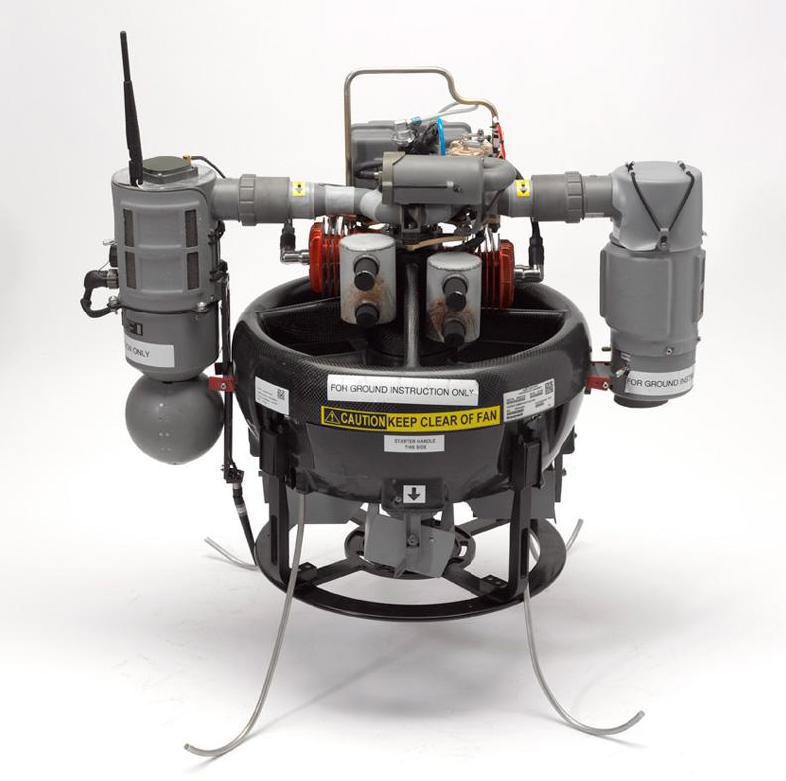
\includegraphics[width=6cm,height=6cm]{Fig/honeywell_t-hawk.jpg}
		\caption{\label{Hawk}T-Hawk}
	\end{minipage}%
	\begin{minipage}[c]{0.5\textwidth}
		\centering
		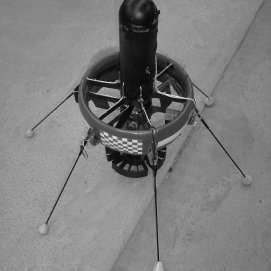
\includegraphics[width=6cm,height=6cm]{Fig/GTSpy.jpg}
		\caption{\label{GTSpy}GTSpy}
	\end{minipage}
\end{figure}
\end{lstlisting}
其中[c]表示行居中对齐。当图片大小不一但又需要1:1导入时,图标题可能行不对齐,因此可以改为如下指令:
\begin{lstlisting}
\begin{figure}[htbp]
	\centering
	\begin{minipage}[c]{0.5\textwidth}
		\centering
		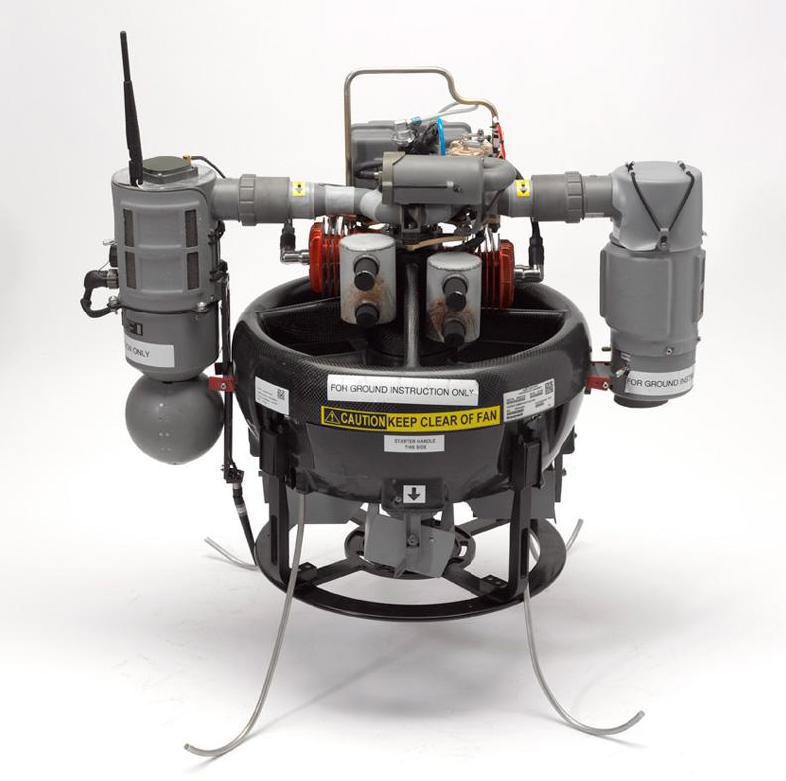
\includegraphics[scale=1]{Fig/honeywell_t-hawk.jpg} %1:1导入
	\end{minipage}%
	\begin{minipage}[c]{0.5\textwidth}
		\centering
		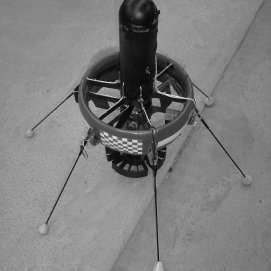
\includegraphics[scale=1]{Fig/GTSpy.jpg}
	\end{minipage}\\[1pt]
	\begin{minipage}[t]{0.5\textwidth}	% 以下为新添加页面划分,[t]表示行顶部对齐
		\caption{\label{Hawk}T-Hawk}
	\end{minipage}%
	\begin{minipage}[t]{0.5\textwidth}
		\caption{\label{GTSpy}GTSpy}
	\end{minipage}%
\end{figure}
\end{lstlisting}
\begin{figure}[htbp]
	\centering
	\begin{minipage}[c]{0.5\textwidth}
		\centering
		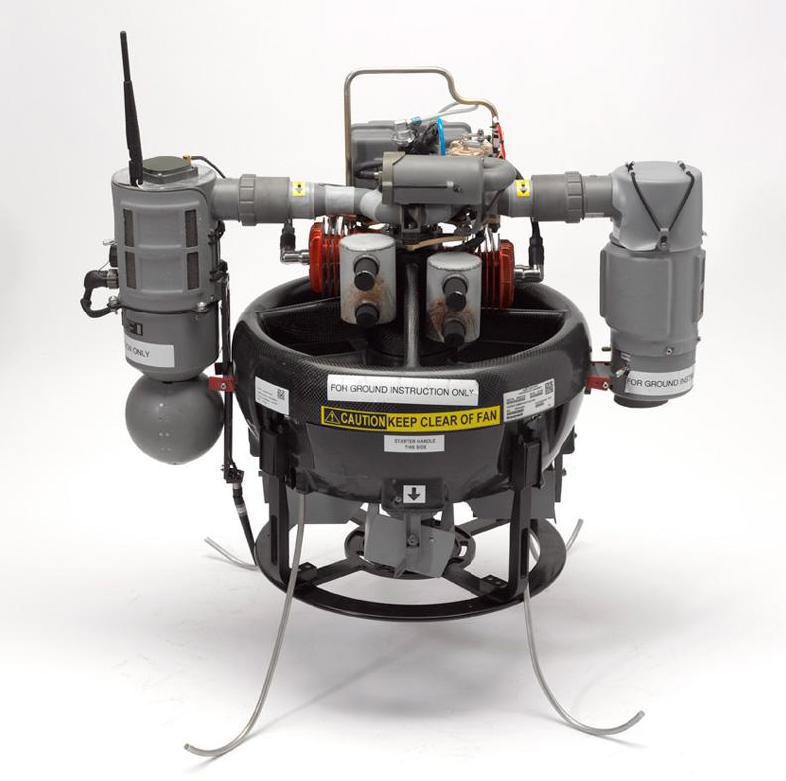
\includegraphics[width=6cm,height=6cm]{Fig/honeywell_t-hawk.jpg}
		\caption{\label{Hawk}T-Hawk}
	\end{minipage}%
	\begin{minipage}[c]{0.5\textwidth}
		\centering
		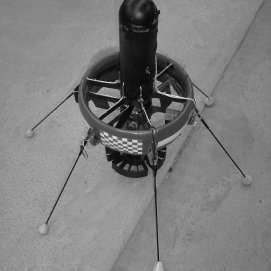
\includegraphics[width=6cm,height=6cm]{Fig/GTSpy.jpg}
		\caption{\label{GTSpy}GTSpy}
	\end{minipage}
\end{figure}


通常一个figure内含有其他小的figure,可以使用一些宏包,但最初本着简单的原则,本模板并没有使用这些子图包。后来应同学们要求在,把子图的功能加上,主要是修改了模板文件(gxuthesis.cls文件)的功能包参数。注意,很多网上拿到的代码不一定可以精确的调子图标题字体字号,因为此模板的子图标题字体字号是利用subfig宏包的选项进行设置的(在gxuthesis.cls文件的“图表环境”中),而有些教程使用subcaption进行同样的设置,还需进一步验证可行性。另外图的排版方法很多,有些宏包已经被弃用,所以尽量使用本文给出的案例的格式进行排版图片。

常见的子图包有subfigure和subfig。subfigure是比较老的了,这里使用subfig包。两个包在使用的时候用法不同,千万不要混淆了,不然可能会报错。subfig包的命令是\textbackslash{}subfloat。这里给出一种使用subfig包的常用排版,如图\ref{Fig:1}的子图\subref{Fig:1:b},其中\subref*{Fig:1:a}的试验并不好(这里测试了交叉引用\textbackslash{}subref\{xxx\}和\textbackslash{}subref*\{xxx\})。必要时也可以排版多行多列的图、调整图之间的间距,具体可百度。

\begin{lstlisting}
\begin{figure}[!h]
	\centering
	\subfloat[不合理的轨迹]{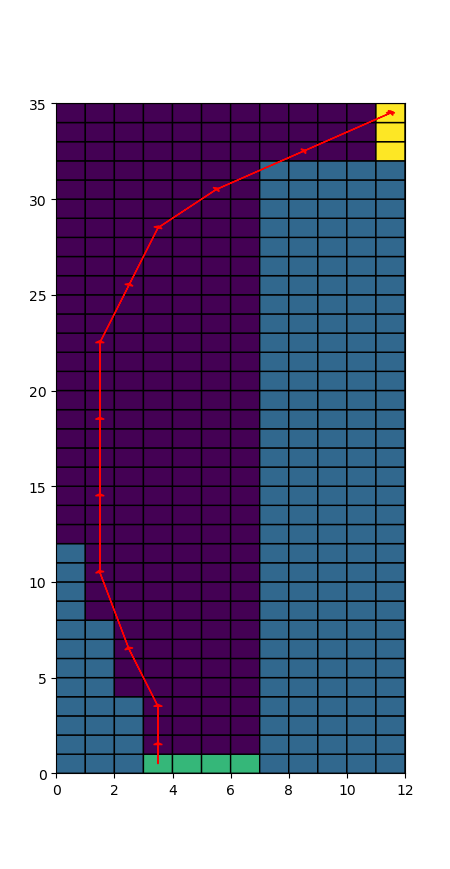
\includegraphics[width=6cm,height=6cm]{Fig/Figure_1.png}%
		\label{Fig:1:a}}
	\subfloat[优化的轨迹]{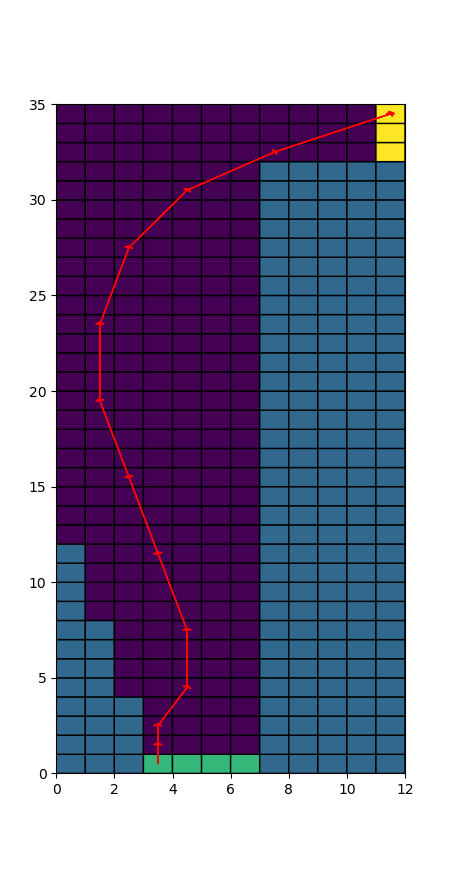
\includegraphics[width=6cm,height=6cm]{Fig/Figure_2.png}
		\label{Fig:1:b}}
	\\ % 用 \\ 换行,也可以此处空一行进行换行,只有两个图的话下面就不需要了。
	\subfloat[不合理的轨迹]{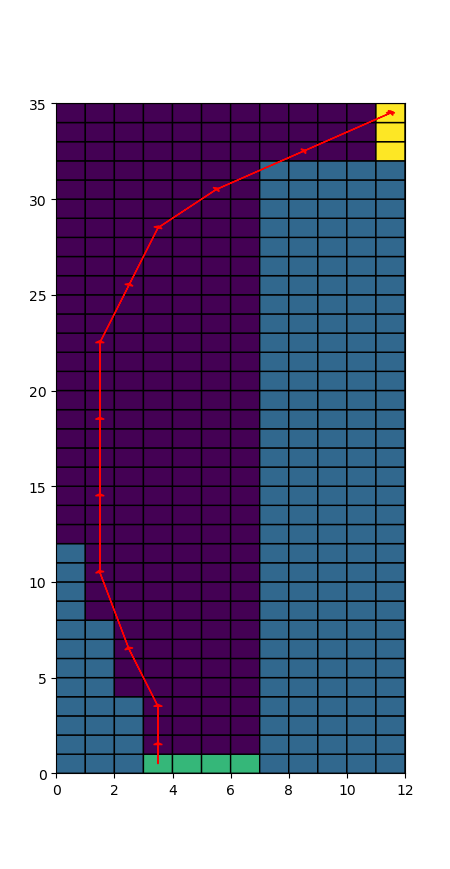
\includegraphics[width=6cm,height=6cm]{Fig/Figure_1.png}%
		\label{Fig:1:c}}
	\subfloat[优化的轨迹]{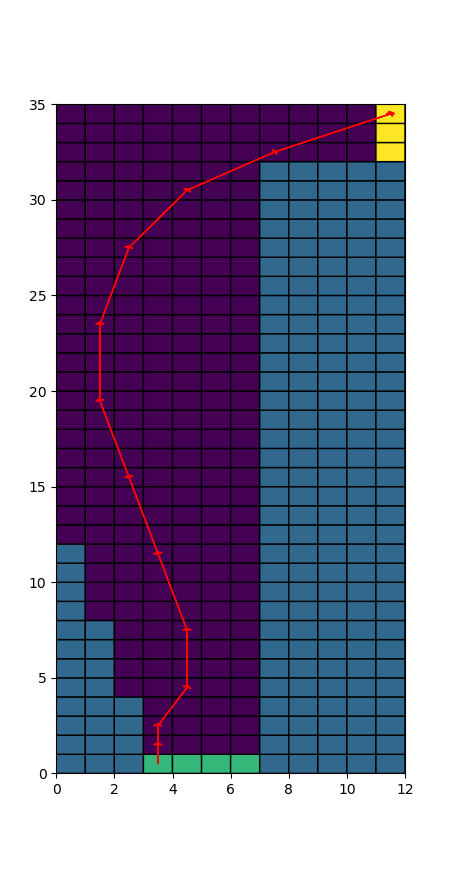
\includegraphics[width=6cm,height=6cm]{Fig/Figure_2.png}%
		\label{Fig:1:d}}
	\caption{子图包使用测试}\label{Fig:1}
\end{figure}
----------------------------------------------------------
% 引用某子图时使用\subref{xxx},其中xxx就是标签Fig:1:a
子图的引用比较特殊,命令有:\subref{xxx}和\subref*{xxx}
注:在subfig包使用说明中,\subref{xxx}和\subref*{xxx}分别由参数listofformat和subrefformat控制,
并由如下定义,根据撰写规范需要定义为:
\DeclareSubrefFormat{empty}{}
\DeclareSubrefFormat{simple}{#1#2}
\DeclareSubrefFormat{parens}{#1 #2)}
\DeclareSubrefFormat{subsimple}{#2}
\DeclareSubrefFormat{subparens}{ #2)}
和
\DeclareCaptionListOfFormat{empty}{}
\DeclareCaptionListOfFormat{simple}{#1#2}
\DeclareCaptionListOfFormat{parens}{#1 #2)}
\DeclareCaptionListOfFormat{subsimple}{#2}
\DeclareCaptionListOfFormat{subparens}{ #2)}
\end{lstlisting}
\begin{figure}[!h]
	\centering
	\subfloat[不合理的轨迹]{\includegraphics[width=6cm,height=6cm]{Fig/Figure_1.png}%
		\label{Fig:1:a}}
	\subfloat[优化的轨迹]{\includegraphics[width=6cm,height=6cm]{Fig/Figure_2.png}
 		\label{Fig:1:b}}
	\\ % 用 \\ 换行,也可以此处空一行进行换行
	\subfloat[不合理的轨迹]{\includegraphics[width=6cm,height=6cm]{Fig/Figure_1.png}%
		\label{Fig:1:c}}
	\subfloat[优化的轨迹]{\includegraphics[width=6cm,height=6cm]{Fig/Figure_2.png}%
		\label{Fig:1:d}}
	\caption{子图包使用测试}\label{Fig:1}
\end{figure}

\section{表}
本节仅展示使用常见的三线表
\begin{lstlisting}
\begin{table}
	\caption{\label{TDF_para}涵道模型参数}	%表题在上
	\centering	% 表居中
	\small	% 表内字体小一号(即设置成和表题字号一致)
	\begin{tabular}{cccc}	% cccc表示4列并居中,若列之间需要分隔符则设置为|c|c|c|c|
		\hline	% \hline表示横线。列之间的元素用&分隔,\tabularnewline表示换行
		参数符号 & 数值 & 参数符号 & 数值 \tabularnewline 
		\hline 
		$I_x$ & $054593$ 		   & $I_y$ & $0.017045         $ \tabularnewline
		$l_1$ & $0.0808\,\text{m}$ & $l_2$ & $0.175\,\text{m}  $ \tabularnewline 
		$l_4$ & $0.2415\,\text{m}$ & $l_5$ & $0.1085\,\text{m} $ \tabularnewline
		\hline 
	\end{tabular}
\end{table}
\end{lstlisting}
\begin{table}
	\caption{\label{TDF_para}涵道模型参数}
	\centering
	\small 
	\begin{tabular}{cccc}
		\hline 
		参数符号 & 数值                & 参数符号 & 数值                 \tabularnewline
		\hline 
		$I_x$   & $054593$ 		     & $I_y$   & $0.017045         $ \tabularnewline
		$l_1$   & $0.0808\,\text{m}$ & $l_2$   & $0.175\,\text{m}  $ \tabularnewline 
		$l_4$   & $0.2415\,\text{m}$ & $l_5$   & $0.1085\,\text{m} $ \tabularnewline
		\hline 
	\end{tabular}
\end{table}

\section{公式}
除了前面讲行内公式,常用的还有行间公式。公式中的数学符号可自行百度,本章仅介绍常用的几种公式环境。

单独成行的行间公式在 \LaTeX{} 里由equation 环境包裹。equation 环境为公式自动生成一个编号,这个编号可以用\textbackslash{}label 和\textbackslash{}ref 生成交叉引用,amsmath 宏包的\textbackslash{}eqref 可为引用自动加上圆括号;如式\eqref{eq_1}所示。
\begin{lstlisting}
\begin{equation}
	a+b=c	\label{eq_1}
\end{equation}
\end{lstlisting}
\begin{equation}
	a+b=c	\label{eq_1}
\end{equation}
若不需要编号则加星号,改为
\begin{lstlisting}
\begin{equation*}
	a+b=c
\end{equation*}
\end{lstlisting}
其他环境类似。当使用 \texttt\$ 开启行内公式输入,或是使用{equation} 环境时,\LaTeX\ 就进入了数学模式。
数学模式相比于文本模式有以下特点:
\begin{enumerate}
	\item 数学模式中输入的空格被忽略。数学符号的间距默认由符号的性质(关系符号、运算符等)决定。
	需要人为引入间距时,使用 \textbackslash{}{quad} 和 \textbackslash{}{qquad} 等命令。
	\item {不允许有空行(分段)}。行间公式中也无法用 $ \verb|\\|$命令手动换行。排版多行公式需要用到 其他各种环境。
	\item 所有的字母被当作数学公式中的变量处理,字母间距与文本模式不一致,也无法生成单词之间的空格。
	如果想在数学公式中输入正体的文本,简单情况下可用 \textbackslash{}{mathrm} 命令。
	或者用 {amsmath} 提供的 \textbackslash{}{text} 命令(仅适合在公式中穿插少量文字。如果你的情况正好相反,需要在许多文字中穿插使用公式,则应该像正常的行内公式那样用,而不是滥用 \textbackslash{}{text} 命令)。
\end{enumerate}	

实际上更常用的的是多行公式,不需要对齐的公式组可以使用gather环境,需要对齐的公式组用align 环境。
长公式内可用$ \verb|\\|$ 换行。

如果需要罗列一系列公式,并令其按照等号对齐,可用align 环境,它将公式用\& 隔为两部分并对齐。分隔符通常放在等号左边:
\begin{lstlisting}
\begin{align}
	a & = b + c \\
	& = d + e
\end{align}
\end{lstlisting}
\begin{align}
a & = b + c \\
& = d + e
\end{align}
align 环境会给每行公式都编号。

如果不需要按等号对齐,只需罗列数个公式,可用gather环境:
\begin{lstlisting}
\begin{gather}
	a  = b + c \notag \\
	f = d + e 
\end{gather}
\end{lstlisting}
\begin{gather}
	a  = b + c \notag  \\
	f = d + e 
\end{gather}
gather 环境同样会给每行公式都编号,如果某行不需要编号可在行末用\textbackslash{}notag 仅去掉某行的编号。

align 和gather 有对应的不带编号的版本align* 和gather*。

另一个常见的需求是将多个公式组在一起公用一个编号,编号位于公式的居中位置。为此,
amsmath 宏包提供了诸如aligned、gathered 等环境,与equation 环境套用。以-ed 结尾的
环境用法与前一节不以-ed 结尾的环境用法一一对应。我们仅以aligned 举例:
\begin{lstlisting}
\begin{equation}
	\begin{aligned}
		a &= b + c \\
		d &= e + f + g \\
		h + i &= j + k \\
		l + m &= n
	\end{aligned}
\end{equation}
\end{lstlisting}
\begin{equation}
	\begin{aligned}
		a &= b + c \\
		d &= e + f + g \\
		h + i &= j + k \\
		l + m &= n
	\end{aligned}
\end{equation}
split 环境和aligned 环境用法类似,也用于和equation 环境套用,区别是split 只能
将每行的一个公式分两栏,aligned 允许每行多个公式多栏。

分段函数通常用amsmath 宏包提供的cases 环境,可参考文献\parencite{_c}

amsmath 宏包还直接提供了多种排版矩阵的环境,包括不带定界符的matrix,以及带各种定界符的矩阵pmatrix、bmatrix、Bmatrix、vmatrix、Vmatrix。
其中中括号版的bmatrix最常用。这些矩阵环境需要在公式中使用,比如 gather 环境。
\begin{lstlisting}
\begin{gather}
	\boldsymbol{A}= \begin{bmatrix}
		x_{11} & x_{12} & \ldots & x_{1n} \\
		x_{21} & x_{22} & \ldots & x_{2n} \\
		\vdots & \vdots & \ddots & \vdots \\
		x_{n1} & x_{n2} & \ldots & x_{nn}
	\end{bmatrix}
\end{gather}
\end{lstlisting}
\begin{gather}
\boldsymbol{A}= \begin{bmatrix}
	x_{11} & x_{12} & \ldots & x_{1n} \\
	x_{21} & x_{22} & \ldots & x_{2n} \\
	\vdots & \vdots & \ddots & \vdots \\
	x_{n1} & x_{n2} & \ldots & x_{nn}
   \end{bmatrix}
\end{gather}	
其中矩阵/向量加粗使用\textbackslash{}boldsymbol\{\}命令,bm宏包的\textbackslash{}bm\{\}命令和unicode-math包有兼容性问题,若使用unicode-math包,就不能使用bm包加粗,unicode-math的一些加粗命令比较特别(具体在math\_font文件夹的测试文件对比差异)。若不使用unicode-math,boldsymbol命令也没法加粗,则再考虑借助bm包。简而言之,公式加粗使用\textbackslash{}boldsymbol\{\}命令。另外还可以使用array环境排版矩阵,类似tabular环境,用$ \verb|\\|$ 和\& 用来分隔行和列,这里不再赘述。	
\begin{lstlisting}
\begin{array }[外部对齐tcb]{列对齐lcr}
	行列内容
\end{array}
\end{lstlisting}

另外注意排版分式时,有两种方法:\textbackslash{}frac或者\textbackslash{}dfrac,效果分别为$ \frac{1}{2} $和$ \dfrac{1}{2} $。以上介绍的数学环境中,空格可参考文献\parencite{_c},例如常用\textbackslash{}quad。

需要局部更改字号时,可以使用tutorial文件夹lshort-zh-cn.pdf的5.1节进行更改,如加\textbackslash{}small使得字号小一号。
\section{定理}
在gxuthesis.cls文件的最后,已经用\textbackslash{}newtheorem命令定义了几种定理环境,包括:定义、假设、定理、结论、引理、公理、推论、性质等等,统称定理环境,关于\textbackslash{}newtheorem的用法,可参考\cite{_g,_c}或自行百度。要下面提供几个例子,在横线之间的深色区域是代码,效果在相应下方表示:
\begin{lstlisting}
\begin{assumption}
	加权矩阵${{\boldsymbol{W}}_{1}}$和 ${{\boldsymbol{W}}_{2}}$ 是对称矩阵,且$ {{\boldsymbol{W}}_{2}}$非奇异。	\label{assum_dca1}
\end{assumption}
\end{lstlisting}
\begin{assumption}
	加权矩阵${{\boldsymbol{W}}_{1}}$和 ${{\boldsymbol{W}}_{2}}$ 是对称矩阵,且$ {{\boldsymbol{W}}_{2}}$非奇异。	\label{assum_dca1}
\end{assumption}

定理用法和假设类似:
\begin{lstlisting}
\begin{theorem}
	如果假设\ref{assum_dca1}成立,$\boldsymbol{F}$满足式\eqref{eq_F}的定义,且${{\boldsymbol{W}}_{1}}$非奇异,则有$0\le e \left( \boldsymbol{F} \right) < 1$,其中$e \left( \boldsymbol{F} \right)$是 $\boldsymbol{F}$的特征值。	\label{the_dca2}
\end{theorem}
\end{lstlisting}
\begin{theorem}
	如果假设\ref{assum_dca1}成立,$\boldsymbol{F}$满足上式的定义,且${{\boldsymbol{W}}_{1}}$非奇异,则有$0\le e \left( \boldsymbol{F} \right) < 1$,其中$e \left( \boldsymbol{F} \right)$是 $\boldsymbol{F}$的特征值。	\label{the_dca2}
\end{theorem}
\begin{remark}
	定理环境的编号可自定义,但通常不需要再进行设置,因为模板文件gxuthesis.cls文件已经定义好。
\end{remark}

---------------------------------------------------------

2022年5月更新:

根据最新的博士论文送审结果,定理等环境统一把原来的斜体改成正体。在此引用一下参考文献\cite{_g}的内容:

amsthm 提供了 \textbackslash{}theoremstyle 命令支持定理格式的切换,在用 \textbackslash{}newtheorem 命令定义定 理环境之前使用。amsthm 预定义了三种格式用于 \textbackslash{}theoremstyle:plain 和 LATEX 原始的格式 一致;definition 使用粗体标签、正体内容;remark 使用斜体标签、正体内容。

以上部分在gxuthesis.cls文件最后一部分设置。

---------------------------------------------------------

amsthm 还提供了一个 proof 环境用于排版定理的证明过程。proof 环境末尾自动加上一个证毕符号:
\begin{proof}
	显然有
	\begin{equation*}
	E=mc^2
	\end{equation*}
	证毕
\end{proof}

proof的大更多用法见参考文献\cite{_g}。gxuthesis.cls文件的最后,跟所有定理环境一样,只是把英文”Proof“改成中文“证明”。

\section{参考文献}

再次强调,使用其他参考文献管理软件的用户以及不使用任何软件的“裸奔”的用户不需要关注任何关于zetero的东西。
\begin{lstlisting}
	关于参考文献这块,很多同学有疑问。只有记住一点:不管用什么参考文献管理工具,最终目的是生成一个bib文件,bib文件里是特定格式的文献信息。bib文件当作文本打开,里面就是文献的元数据。
\end{lstlisting}

通常学位论文参考文献是基于BibTeX进行的,本模板使用的是BibLaTeX,或者叫Biber。关于这部分知识可参考文献\parencite{_c,_g}的第六章,6.1节参考文献和BIBTEX工具。所以使用TeXstudio或者vscode的时候需要注意调整正确的参数进行编译。

引用前手动加空格,如:

引用前没有加空格\parencite{_c,_g}的第六章,引用后面有空格。

引用前手动加空格 \parencite{_c,_g}的第六章,引用后面有空格。

手写方括号 [6]。引用后面没空格。

生成方括号 \parencite{_k}。引用后面没空格。


参考文献引用和著录是基于ZOTERO这个软件进行的。视频教程见\parencite{_k}。此外,为了符合毕业论文撰写规范,需设置参数。按照视频教程安装完必要的插件(如Better BibTeX)后,在编辑->首选项进行设置。图\ref{op1}到图\ref{op11}所示的是我的zotero软件设置。其中最重要的是\ref{op10}的设置要排除的选项,多余的显示会让审稿人反感,按照论文撰写规范进行即可。在毕业论文撰写时,在编辑->首选项->Better BibLTeX->Fields中,Fields to omit from export填month,abstract,note,extra,file,keywords,type,url,doi,就是在参考文献著录中排除这些多余的项,避免过于复杂。而在写本模板使用说明时,没有排除url,因为很多参考资料是网页。

\begin{lstlisting}
    使用zotero,有时候科学上网很重要。
\end{lstlisting}

在zotero软件点击文件->导出文献库,如图\ref{output}所示,再在导出对话框图\ref{output_format}选择导出格式为Better BibLaTeX,同时勾选Keep updated选项保持自动更新,再点击ok,在弹出的对话框图\ref{output_name}确定保存路径和文件名,例如我的是MyLibrary.bib,这也是我整个读书生涯的文献库bib文件。如果写小论文的话通常导出格式是BibTeX或者Better BibTeX(这里按照期刊的要求来即可,文献管理软件的好处就是快速自动生成一个文件库)。关于BibTeX和BibLaTeX的区别这里不做展开。

得到文献库后,在gxuthesis.tex文件第九行使用\textbackslash{}addbibresource命令,添加文献库。引用某文献时秩序在zotero选中某文献条目,然后按Ctrl+Shift+C,复制引用关键字(Citation Key)到剪切板(快捷键可自定义)。然后在tex文件编辑界面直接粘贴,默认的时上标形式,若需要非上标形式,可以改为\textbackslash{}parencite\{xxx\},其中xxx是Citation Key。这里的操作和认为设置的首选项参数有关,需要在编辑->首选项->导出界面的默认格式一栏选中相应的项,同时在编辑->首选项->高级->快捷键设置为默认值。

---------------------------------------------------------------------------------

2020年12月2日测试:
下载最新zotero,从知网和谷歌捕获文献(刚打开网页最好稍等一会再点击插件,谷歌可能需要现人机验证),对文献\parencite{Renduchintala_2019}、\parencite{milz2020design}进行引用。

---------------------------------------------------------------------------------

---------------------------------------------------------------------------------

2021年9月14日测试:
使用endnote的用户也可以利用导出的bib文件生成参考文献著录信息,导出选项是bibTeX,貌似没有更多导出设置选项。导出设置没有zotero那么灵活丰富,得到bib文件后要引用某论文需要自行查找标签(label,也有软件叫引用关键字Citation Key)\{xxx\}然后手打\textbackslash{}cite\{xxx\}。欢迎熟悉endnote的同学来信告诉我更好的办法。

---------------------------------------------------------------------------------

2023年3月8日测试:参考文献管理软件经常更新,但还是那句话,无论什么工具,最终得到bib文件即可,在期刊的文章页或者谷歌学术搜索页,只需要复制/下载bibtex的内容。得到这些元数据后甚至自己往bib文件里加都可以。

---------------------------------------------------------------------------------

2023年11月测试。论文写完记得断掉bib文件自动更新,在zotero的插件Better BibTeX自动导出设置里删除不希望再继续同步到项。否则更改软件中的文献后,论文的bib文件也同步更改,但有时候这不是想要的。
\begin{lstlisting}
    另外有同学反映,换了电脑后重新导出的bib文件Citation Key值不同,记得设置好Better BibTeX之后,在著录条目界面全选著录(或仅选想更新的著录)然后右键选Better BibTeX更新refresh一下。然后在Automatic export选项点击Export now立即更新bib文件(按理说勾选了自动更新选项他会自动更新,但为了确保万无一失还是点一下)。
\end{lstlisting}
\begin{figure}
	\centering
	\includegraphics[scale=0.8]{Fig/zotero1.png}
	\caption{\label{op1}常规}
\end{figure}
\begin{figure}
	\centering
	\includegraphics[scale=0.8]{Fig/zotero2.png}
	\caption{\label{op2}同步1}
\end{figure}
\begin{figure}
	\centering
	\includegraphics[scale=0.8]{Fig/zotero3.png}
	\caption{\label{op3}同步2}
\end{figure}
\begin{figure}
	\centering
	\includegraphics[scale=0.8]{Fig/zotero4.png}
	\caption{\label{op4}搜索}
\end{figure}
\begin{figure}
	\centering
	\includegraphics[scale=0.8]{Fig/zotero5.png}
	\caption{\label{op5}导出}
\end{figure}
\begin{figure}
	\centering
	\includegraphics[scale=0.8]{Fig/zotero6.png}
	\caption{\label{op6}引用}
\end{figure}
\begin{figure}
	\centering
	\includegraphics[scale=0.8]{Fig/zotero7.png}
	\caption{\label{op7}高级1}
\end{figure}
\begin{figure}
	\centering
	\includegraphics[scale=0.8]{Fig/zotero8.png}
	\caption{\label{op8}高级2}
\end{figure}
\begin{figure}
	\centering
	\includegraphics[scale=0.8]{Fig/zotero9.png}
	\caption{\label{op9}Better BibTeX1}
\end{figure}
\begin{figure}
	\centering
	\includegraphics[scale=0.8]{Fig/zotero10.png}
	\caption{\label{op10}Better BibTeX2}
\end{figure}
\begin{figure}
	\centering
	\includegraphics[scale=0.8]{Fig/zotero11.png}
	\caption{\label{op11}Better BibTeX3}
\end{figure}

\begin{figure}[htbp]
	\centering
	\includegraphics[scale=0.42]{Fig/zotero12.png}
	\caption{\label{output}导出文献库}
\end{figure}

\begin{figure}[htbp]
	\centering
	\includegraphics[scale=0.42]{Fig/zotero13.png}
	\caption{\label{output_format}导出格式}
\end{figure}

\begin{figure}[htbp]
	\centering
	\includegraphics[scale=0.42]{Fig/zotero14.png}
	\caption{\label{output_name}导出文件名}
\end{figure}









 % 第三章
% 自行根据需要添加章节。
...
\chapter{结\texorpdfstring{\quad}{}论}
本文主要是展示如何使用修改“祖传模板”得到的新模板,在使用时直接替换成自己的论文内容即可。

本模板难免有不足之处,主要是我本人的论文涉及的格式有限,有些地方没探索到自然就没去设置。比如附录,附录的图文并茂等等,我本人是没有研究的,这里仅仅做了一些初步的工作,不过对很多同学来说本模板是够用的。希望有能帮助到华工的同学们,有不足之处请多多理解,可以通过邮件联系我,我会尽量回复。
 % 结论
...
\printbibliography	% 参考文献著录
%%%%%%%%%%%%%%%%%%%此部分为附录环境代码,是比较笨的方法来适应论文撰写规范%%%%%%%%%%%%%%%%%%%%%%%%%%%%%%%%%%%%%%
%对只有一个附录,标题不编号比较美观。
%%%%%%%%%%%%%%%%%%%%%%%%%%%%%%%%%%%%%%%%%%%%%%%%%%%%%%%%%%%%%%%%%%%%%%%%%%%%%%%%%%%%%%%%%%%%%%%%%%%%%%%%%%%%
\setcounter{chapter}{1} %从1开始编号
\setcounter{section}{0}
\setcounter{equation}{0}
\setcounter{table}{0}   
\setcounter{figure}{0}
\chapter{附\texorpdfstring{\quad}{}录} %附录
%%%%%%%%%%%%%%%%%%%%%%%%%%%%%%%%%%%%%%%%%%%%%%%%%%%%%%%%%%%%%%%%%%%%%%%%%%%%%%%%%%%%%%%%%%%%%%%%%%%%%%%%
%%%%%%%%%%%%以下为用户代码,用于撰写您的论文%%%%%%%%%%%%%%%%%%%%%%%%%%%%%%%%%%%%%%%%%%%%%%%%%%%%%%%%%%%%%%


在论文撰写规范中,下面两段话让人费解:

\begin{enumerate}
	\item 	对需要收录于学位论文中但又不适合书写于正文中的附加数据、方案、资料、详细公式推导、计算机程序、统计表、注释等有特色的内容,可做为附录排写,序号采用“附录1”、“附录2”等。	
	\item	公式序号按章编排,如第一章第一个公式序号为“(1-1)”,附录2中的第一个公式为“(2-1)”等。
\end{enumerate}

论文撰写规范要求的附录和通常书籍上使用附录A、附录B等编号的不一样,容易和正文混淆。特殊的要求和代码的耦合,使我不得不使用比较笨的方法来设计附录部分的模板。

\section{测试测试测试}
\subsection{测试测试测试}
%
测试测试测试测试测试测试测试测试测试测试测试测试测试测试测试测试测试测试测试测试测试测试测试测试测试测试测试测试测试测试测试测试测试测试测试测试测试测试测试测试测试测试测试测试测试测试测试测试测试测试测试测试测试测试测试测试测试测试测试测试测试测试测试测试测试测试测试测试测试测试测试测试测试测试测试测试测试测试测试测试测试测试测试测试测试测试测试测试测试测试测试测试测试测试测试测试测试测试测试测试测试测试测试测试测试测试测试测试测试测试测试测试测试测试测试测试测试测试测试测试测试测试测试测试测试测试测试测试测试测试测试测试测试测试测试测试测试测试测试测试测试测试测试测试测试测试测试测试测试测试测试测试测试
\begin{align}
\left\{\begin{array}{l}
\dot{v}_{1}(t)=v_{2}(t) \\
\dot{v}_{2}(t)=R^{2}\left(-\zeta_{1}\left[v_{1}(t)-v_c(t)\right]^{\alpha}-\zeta_{2}\left[\dfrac{v_{2}(t)}{R}\right]^{\beta}\right)
\end{array}\right.	
\end{align}

\begin{align}
\left\{\begin{array}{l}
\dot{v}_{1}(t)=v_{2}(t) \\
\dot{v}_{2}(t)=R^{2}\left(-\zeta_{1}\left[v_{1}(t)-v_c(t)\right]^{\alpha}-\zeta_{2}\left[\dfrac{v_{2}(t)}{R}\right]^{\beta}\right)
\end{array}\right.	
\end{align}
\begin{figure}[htbp]
	\centering	
	\includegraphics[scale=1]{Fig/DFUAV_f31.png}
	\caption{\label{fig_case1}测试测试测试}
\end{figure}
\begin{figure}[htbp]
	\centering	
	\includegraphics[scale=1]{Fig/DFUAV_f31.png}
	\caption{\label{fig_case2}测试测试测试}
\end{figure}
\begin{table}
	\caption{\label{DF_para1}测试测试测试}
	\centering{}%
	\small 
	\begin{tabular}{cccccc}
		\hline 
		参数符号 & 数值&参数符号 & 数值&参数符号 & 数值\tabularnewline
		\hline 
		$ A_x,A_y,A_z $  & $ 0.04082\,\text{m}^2 $ &$ \rho $        &$1.225\,\text{kg}/\text{m}^3$&$ I_b $           & $ 0.000029 $               \tabularnewline
		$ k_{\varpi} $   & $1.13342 \times 10^{-6}$& $ d_{\varpi} $ & $1.13342 \times 10^{-7}$ 	  &$k_{\delta} $     & $ 0.01495 $ 			      \tabularnewline
		$C_{D,x},C_{D,y}$& $ 0.43213 $             &$ C_{D,z} $     & $ 0.13421 $             	  &	$ q_a $ 	     & $ 1.49 $ 				  \tabularnewline
		$ l_{a} $        & $ -0.1121\,\text{m} $   & $ d_{ds} $     & $ 0.01495 $			  	  &$ d_{af} $        & $ 0.01495 $    			  \tabularnewline
		$ R $            & $ 0.11\,\text{m} $      &$ b $           & $ 2 $       			   	  &$ S $ 			 & $ 0.04082\,\text{m}^2 $    \tabularnewline
		$C_{l_{\alpha}}$ & $ 2.212\,/\text{rad} $  &$C_{l, \max } $ & $ 1.05 $ 				   	  &$ C_{l, \min } $  & $ -1.05 $ 				  \tabularnewline
		$ l_2 $          & $ 0.06647\,\text{m} $   &$ l_1 $         & $ 0.17078\,\text{m} $    	  &	$ m $ 		     & $ 1.53\,\text{kg} $ 		  \tabularnewline
		$ C_{d, o } $    & $ 0.9 $                 &$ C_{d, g } $   & $ 0.9 $					  &$ C_{duct} $      & $ 0.78497 $	 			  \tabularnewline
		$ I_x $          & $ 0.02548 $ 			   &$ I_y $         & $ 0.02550 $                 &$ I_z $			 & $ 0.00562 $ 				  \tabularnewline
		\hline 
	\end{tabular}	
\end{table}

\begin{table}
	\caption{\label{TDF_para2}测试测试测试}
	\centering{}%
	\small 
	%	\resizebox{\textwidth}{!}{
	\begin{tabular}{cccccc}
		\hline 
		参数符号 & 数值&参数符号 & 数值&参数符号 & 数值\tabularnewline
		\hline 
		$ I_x $ & $ 054593 $ &$ I_y $ & $ 0.017045 $& $ I_z$ & $ 0.049226 $ \tabularnewline
		$ l_{1} $ & $ 0.0808\,\text{m} $&$ l_{2} $ & $ 0.175\,\text{m} $ &$ l_3 $ & $ 0.06647\,\text{m} $ \tabularnewline 
		$ l_4 $ & $ 0.2415\,\text{m} $ &$ l_5 $ & $ 0.1085\,\text{m} $& $ m $ & $ 3.7\,\text{kg} $ \tabularnewline
		\hline 
	\end{tabular}	%}
\end{table}

\section{测试测试测试}
\subsection{测试测试测试}
%
测试测试测试测试测试测试测试测试测试测试测试测试测试测试测试测试测试测试测试测试测试测试测试测试测试测试测试测试测试测试测试测试测试测试测试测试测试测试测试测试测试测试测试测试测试测试测试测试测试测试测试测试测试测试测试测试测试测试测试测试测试测试测试测试测试测试测试测试测试测试测试测试测试测试测试测试测试测试测试测试测试测试测试测试测试测试测试测试测试测试测试测试测试测试测试测试测试测试测试测试测试测试


 % 附录
\chapter{攻读学位期间发表论文与研究成果清单} % 
\pubfont %  


\begin{enumerate}[topsep = 0 pt, itemsep= 0 pt, parsep=0pt, partopsep=0pt, leftmargin=44pt, itemindent=0pt, labelsep=6pt, label=(\arabic*)]
	\item 论文1:
	\item 
 


\end{enumerate}

\normalsize % \normalsize可以将下文调回和正文一样的字号,这个随个人喜好。注释掉的话,致谢就就跟随《攻读博士/硕士学位期间取得的研究成果》的字号。 % 成果
\chapter{致\texorpdfstring{\quad}{}谢}
%把下面文字替换
\begin{center}
这次你离开了没有像以前那样说再见,再见也他妈的只是再见 
~\\
我们之间从来没有想象的那么接近,只是两棵树的距离 
~\\
你是否还记得山阴路我八楼的房间,房间里唱歌的日日夜夜 
~\\
那么热的夏天你看着外面,看着你在消逝的容颜 
~\\
我多么想念你走在我身边的样子,想起来我的爱就不能停止 
~\\
南京的雨不停地下不停地下,就像你沉默的委屈 
~\\
一转眼,我们的城市又到了夏天,对面走来的人都眯着眼 
~\\
人们不敢说话不敢停下脚步,因为心动常常带来危险 
~\\
我多么想念你走在我身边的样子,想起来我的爱就不能停止 
~\\
南京的雨不停地下不停地下,有些人却注定要相遇 
~\\
你是一片光荣的叶子,落在我卑贱的心 
~\\
像往常一样我为自己生气并且歌唱 
~\\
那么乏力,爱也吹不动的叶子 
\end{center}
%把上面文字替换

~\\

\begin{minipage}[t]{0.945\textwidth}%
	\begin{flushright}
		作者姓名\\
%		\today\\	% 自动时间
		2020年7月10日\\	%固定时间
		于华南理工大学
		\par\end{flushright}
\end{minipage}

 % 致谢
\end{lstlisting}
其中$\%$之后的内容为注释,...表示省略其他代码,仅保留论文内容主体部分。\textbackslash{}include\{xxx\}指令用于包含xxx.tex文件的内容,各章节的内容主要在xxx.tex中保存。在\textbackslash{}documentclass 和\textbackslash{}begin\{document\} 之间的位置称为导言区。在导言区中一般会使用\textbackslash{}usepackage 调用宏包,以及会进行对文档的全局设置。本模板的导言区除调用所需的宏包外,还进行了页眉页脚的设置。有的模板会把所有调用宏包的指令放到一个.sty宏包文件中,页面的设置放在文档类文件.cls文件中。因本人时间有限,就不做整理,欢迎有志之士加入完善。使用本模板并不需要了解导言区的指令,在需要时额外添加即可(要注意宏包冲突)。特别地,\textbackslash{}includeonly\{xxx\}指令用于使文档仅编译xxx.tex文件的内容,这就是分章节包含(include)的好处,可大大减少编译时间。

将封面打印保存为 thesis\_cover.pdf 文件,硕士使用master\_cover.docx ,博士使用 doctor\_cover.doc 。如果有更新版本的封面,可自行替换。文档类默认是博士论文,下面指令将控制添加封面与否:
\begin{lstlisting}
\documentclass[unicode,master,pdfcover]{gxuthesis}	% 使用pdf文件封面的 硕士模板
\documentclass[unicode,master]{gxuthesis}	% 不使用pdf文件封面的 硕士模板
\documentclass[unicode,pdfcover]{gxuthesis}	% 使用pdf文件封面的博士模板
\documentclass[unicode]{gxuthesis}	% 不使用pdf文件封面的博士模板
\end{lstlisting}
不使用thesis\_cover.pdf 文件指定的封面时,将使用草稿封面。草稿封面也可以减少编译时间,因此可以在最终提交论文时再使用论文封面。草稿封面用以下指令设置:
\begin{lstlisting}
%%%%%%%%%%%%%草稿封面设置%%%%%%%%%%%%%	
\title{LaTeX模板}	
\author{作者姓名}	
\supervisor{指导教师:xxx\ 教授}	
\institute{华南理工大学}	
\date{2020年5月20日}
%%%%%%%%%%%%%%%%%%%%%%%%%%%%%%%%%%%%%
\end{lstlisting}
\section{章节文件}
chapter文件夹的章节文件如chapter0x.tex等,其内容由\textbackslash{}chapter\{章名\}开头。新建一章可新建一个文件并由\textbackslash{}chapter\{新建章名\}开头填写内容即可。节及小节分别用\textbackslash{}section\{新建节名\}、\textbackslash{}subsection\{新建小节名\}命令。

正文的的书写和txt文本文件的书写类似。\LaTeX{} 源代码中,空格键和Tab键输入的空白字符视为“空格”。连续的若干个空白字符视为一个空格。一行开头的空格忽略不计。行末的回车视为一个空格;但连续两个回车,也就是空行,会将文字分段。多个空行被视为一个空行。也可以在行末使用\textbackslash{}par 命令分段。在本模板中,英文之间的空格被保留,中文之间的空格被忽略。特别地,摘要,附录,结论等两个字的大纲级别为章的章名,中间使用空格隔开。对此论文撰写规范并没有明文要求,只是为了美观。也可以全部不加空格。一般情况下,在文本文字中添加空格使用\textbackslash{}quad命令,但由于文献\parencite{_d}所述原因,直接使用\textbackslash{}quad命令会报警,因而使用\textbackslash{}texorpdfstring\{\textbackslash{}quad\}\{\},其中最后一个\{\}里面可以加一个空格,不影响使用。目录二字之间添加空格在gxuthesis.cls文件317行设置。

正文本环境中使用公式,即行内公式,需要用两个\$包围,如源码:\$a+b=c\$ 显示为$a+b=c$。使用其他字符可自行百度或阅读参考文献。再次提醒,使用\LaTeX{}撰写论文不需要研究其原理,在达到某种效果(图文显示、公式显示效果)时百度或查书寻找其代码即可。

综上,论文撰写只需要将自己的文本(包含行内公式)放到相应的章节处,并添加行间公式、图表环境并填写图表即可。行间公式、图表将在下一章介绍。

%第二章
	
\chapter{常用环境及参考文献设置}
强烈建议在使用公式、表格、定理环境时进行百度,没必要研究各种用法,只需要知道自己需要什么。因本人的论文所用表格较少,因而对表格不是很熟悉,本章对表格的介绍相应的较少。本章仅介绍本人在论文撰写过程中常用的环境以及参考文献设置。

\section{图}
图的导入需要提前准备好图片文件,最好是.png、.eps、.pdf或.jpg文件。另外,如果是从matlab导出图片文件,可使用print函数或手动导出,print函数的使用可参考ICGNC2020plot.m以及PlotToFileColorPDF.m文件等。手动导出(matlab的figure界面的“文件”->“导出设置”设置好大小、分辨率和线宽等然后点击“应用于图窗”)主要用于观察效果,可设置某种样式名称后保存该样式,下次使用时加载,具体可百度“matlab导出高清图片”。需要特别注意的是一定要1:1导入matlab生成的图片,并且图中文字设置好字体字号。否则缩放之后,图片的字号就变了,盲审老师一眼就能看出来字号不对,就很麻烦。这就是为什么要在matlab点击“应用于图窗“进行预览,观测效果后再1:1使用图片。

使用如下代码放置独立成行的图片,效果如图\ref{one_DFUAV}所示
\begin{lstlisting}
\begin{figure}[htbp]
	% 图片居中(列居中对齐)
	\centering	
	% 包含当前路径下的Fig文件夹的图片文件DFUAV_f31.png
	\includegraphics[scale=1]{Fig/DFUAV_f31.png} 
	% 添加标签one_DFUAV以及图标题“涵道风扇式无人机”,引用某图时使用\ref{xxx},其中xxx就是标签,图编号是自动生成的。
	\caption{\label{one_DFUAV}涵道风扇式无人机} 
\end{figure}
\end{lstlisting}
其中figure为环境名,[htbp]表示将图片设置为浮动体,实际上这在.cls文件已经设置过,因而可以省略。[scale=1]表示安装1:1的比例导入图片,还可以按其他方式导入,需要时可自行百度。
\begin{figure}[htbp]
	\centering
	\includegraphics[scale=1]{Fig/DFUAV_f31.png}
	\caption{\label{one_DFUAV}涵道风扇式无人机}
\end{figure}

使用如下代码划分页面并排放置图\ref{Hawk}、图\ref{GTSpy}
\begin{lstlisting}
\begin{figure}[htbp]
	\centering
	\begin{minipage}[c]{0.5\textwidth} % minipage将页面划分为0.5\textwidth
		\centering
		\includegraphics[width=6cm,height=6cm]{Fig/honeywell_t-hawk.jpg}
		\caption{\label{Hawk}T-Hawk}
	\end{minipage}%
	\begin{minipage}[c]{0.5\textwidth}
		\centering
		\includegraphics[width=6cm,height=6cm]{Fig/GTSpy.jpg}
		\caption{\label{GTSpy}GTSpy}
	\end{minipage}
\end{figure}
\end{lstlisting}
其中[c]表示行居中对齐。当图片大小不一但又需要1:1导入时,图标题可能行不对齐,因此可以改为如下指令:
\begin{lstlisting}
\begin{figure}[htbp]
	\centering
	\begin{minipage}[c]{0.5\textwidth}
		\centering
		\includegraphics[scale=1]{Fig/honeywell_t-hawk.jpg} %1:1导入
	\end{minipage}%
	\begin{minipage}[c]{0.5\textwidth}
		\centering
		\includegraphics[scale=1]{Fig/GTSpy.jpg}
	\end{minipage}\\[1pt]
	\begin{minipage}[t]{0.5\textwidth}	% 以下为新添加页面划分,[t]表示行顶部对齐
		\caption{\label{Hawk}T-Hawk}
	\end{minipage}%
	\begin{minipage}[t]{0.5\textwidth}
		\caption{\label{GTSpy}GTSpy}
	\end{minipage}%
\end{figure}
\end{lstlisting}
\begin{figure}[htbp]
	\centering
	\begin{minipage}[c]{0.5\textwidth}
		\centering
		\includegraphics[width=6cm,height=6cm]{Fig/honeywell_t-hawk.jpg}
		\caption{\label{Hawk}T-Hawk}
	\end{minipage}%
	\begin{minipage}[c]{0.5\textwidth}
		\centering
		\includegraphics[width=6cm,height=6cm]{Fig/GTSpy.jpg}
		\caption{\label{GTSpy}GTSpy}
	\end{minipage}
\end{figure}


通常一个figure内含有其他小的figure,可以使用一些宏包,但最初本着简单的原则,本模板并没有使用这些子图包。后来应同学们要求在,把子图的功能加上,主要是修改了模板文件(gxuthesis.cls文件)的功能包参数。注意,很多网上拿到的代码不一定可以精确的调子图标题字体字号,因为此模板的子图标题字体字号是利用subfig宏包的选项进行设置的(在gxuthesis.cls文件的“图表环境”中),而有些教程使用subcaption进行同样的设置,还需进一步验证可行性。另外图的排版方法很多,有些宏包已经被弃用,所以尽量使用本文给出的案例的格式进行排版图片。

常见的子图包有subfigure和subfig。subfigure是比较老的了,这里使用subfig包。两个包在使用的时候用法不同,千万不要混淆了,不然可能会报错。subfig包的命令是\textbackslash{}subfloat。这里给出一种使用subfig包的常用排版,如图\ref{Fig:1}的子图\subref{Fig:1:b},其中\subref*{Fig:1:a}的试验并不好(这里测试了交叉引用\textbackslash{}subref\{xxx\}和\textbackslash{}subref*\{xxx\})。必要时也可以排版多行多列的图、调整图之间的间距,具体可百度。

\begin{lstlisting}
\begin{figure}[!h]
	\centering
	\subfloat[不合理的轨迹]{\includegraphics[width=6cm,height=6cm]{Fig/Figure_1.png}%
		\label{Fig:1:a}}
	\subfloat[优化的轨迹]{\includegraphics[width=6cm,height=6cm]{Fig/Figure_2.png}
		\label{Fig:1:b}}
	\\ % 用 \\ 换行,也可以此处空一行进行换行,只有两个图的话下面就不需要了。
	\subfloat[不合理的轨迹]{\includegraphics[width=6cm,height=6cm]{Fig/Figure_1.png}%
		\label{Fig:1:c}}
	\subfloat[优化的轨迹]{\includegraphics[width=6cm,height=6cm]{Fig/Figure_2.png}%
		\label{Fig:1:d}}
	\caption{子图包使用测试}\label{Fig:1}
\end{figure}
----------------------------------------------------------
% 引用某子图时使用\subref{xxx},其中xxx就是标签Fig:1:a
子图的引用比较特殊,命令有:\subref{xxx}和\subref*{xxx}
注:在subfig包使用说明中,\subref{xxx}和\subref*{xxx}分别由参数listofformat和subrefformat控制,
并由如下定义,根据撰写规范需要定义为:
\DeclareSubrefFormat{empty}{}
\DeclareSubrefFormat{simple}{#1#2}
\DeclareSubrefFormat{parens}{#1 #2)}
\DeclareSubrefFormat{subsimple}{#2}
\DeclareSubrefFormat{subparens}{ #2)}
和
\DeclareCaptionListOfFormat{empty}{}
\DeclareCaptionListOfFormat{simple}{#1#2}
\DeclareCaptionListOfFormat{parens}{#1 #2)}
\DeclareCaptionListOfFormat{subsimple}{#2}
\DeclareCaptionListOfFormat{subparens}{ #2)}
\end{lstlisting}
\begin{figure}[!h]
	\centering
	\subfloat[不合理的轨迹]{\includegraphics[width=6cm,height=6cm]{Fig/Figure_1.png}%
		\label{Fig:1:a}}
	\subfloat[优化的轨迹]{\includegraphics[width=6cm,height=6cm]{Fig/Figure_2.png}
 		\label{Fig:1:b}}
	\\ % 用 \\ 换行,也可以此处空一行进行换行
	\subfloat[不合理的轨迹]{\includegraphics[width=6cm,height=6cm]{Fig/Figure_1.png}%
		\label{Fig:1:c}}
	\subfloat[优化的轨迹]{\includegraphics[width=6cm,height=6cm]{Fig/Figure_2.png}%
		\label{Fig:1:d}}
	\caption{子图包使用测试}\label{Fig:1}
\end{figure}

\section{表}
本节仅展示使用常见的三线表
\begin{lstlisting}
\begin{table}
	\caption{\label{TDF_para}涵道模型参数}	%表题在上
	\centering	% 表居中
	\small	% 表内字体小一号(即设置成和表题字号一致)
	\begin{tabular}{cccc}	% cccc表示4列并居中,若列之间需要分隔符则设置为|c|c|c|c|
		\hline	% \hline表示横线。列之间的元素用&分隔,\tabularnewline表示换行
		参数符号 & 数值 & 参数符号 & 数值 \tabularnewline 
		\hline 
		$I_x$ & $054593$ 		   & $I_y$ & $0.017045         $ \tabularnewline
		$l_1$ & $0.0808\,\text{m}$ & $l_2$ & $0.175\,\text{m}  $ \tabularnewline 
		$l_4$ & $0.2415\,\text{m}$ & $l_5$ & $0.1085\,\text{m} $ \tabularnewline
		\hline 
	\end{tabular}
\end{table}
\end{lstlisting}
\begin{table}
	\caption{\label{TDF_para}涵道模型参数}
	\centering
	\small 
	\begin{tabular}{cccc}
		\hline 
		参数符号 & 数值                & 参数符号 & 数值                 \tabularnewline
		\hline 
		$I_x$   & $054593$ 		     & $I_y$   & $0.017045         $ \tabularnewline
		$l_1$   & $0.0808\,\text{m}$ & $l_2$   & $0.175\,\text{m}  $ \tabularnewline 
		$l_4$   & $0.2415\,\text{m}$ & $l_5$   & $0.1085\,\text{m} $ \tabularnewline
		\hline 
	\end{tabular}
\end{table}

\section{公式}
除了前面讲行内公式,常用的还有行间公式。公式中的数学符号可自行百度,本章仅介绍常用的几种公式环境。

单独成行的行间公式在 \LaTeX{} 里由equation 环境包裹。equation 环境为公式自动生成一个编号,这个编号可以用\textbackslash{}label 和\textbackslash{}ref 生成交叉引用,amsmath 宏包的\textbackslash{}eqref 可为引用自动加上圆括号;如式\eqref{eq_1}所示。
\begin{lstlisting}
\begin{equation}
	a+b=c	\label{eq_1}
\end{equation}
\end{lstlisting}
\begin{equation}
	a+b=c	\label{eq_1}
\end{equation}
若不需要编号则加星号,改为
\begin{lstlisting}
\begin{equation*}
	a+b=c
\end{equation*}
\end{lstlisting}
其他环境类似。当使用 \texttt\$ 开启行内公式输入,或是使用{equation} 环境时,\LaTeX\ 就进入了数学模式。
数学模式相比于文本模式有以下特点:
\begin{enumerate}
	\item 数学模式中输入的空格被忽略。数学符号的间距默认由符号的性质(关系符号、运算符等)决定。
	需要人为引入间距时,使用 \textbackslash{}{quad} 和 \textbackslash{}{qquad} 等命令。
	\item {不允许有空行(分段)}。行间公式中也无法用 $ \verb|\\|$命令手动换行。排版多行公式需要用到 其他各种环境。
	\item 所有的字母被当作数学公式中的变量处理,字母间距与文本模式不一致,也无法生成单词之间的空格。
	如果想在数学公式中输入正体的文本,简单情况下可用 \textbackslash{}{mathrm} 命令。
	或者用 {amsmath} 提供的 \textbackslash{}{text} 命令(仅适合在公式中穿插少量文字。如果你的情况正好相反,需要在许多文字中穿插使用公式,则应该像正常的行内公式那样用,而不是滥用 \textbackslash{}{text} 命令)。
\end{enumerate}	

实际上更常用的的是多行公式,不需要对齐的公式组可以使用gather环境,需要对齐的公式组用align 环境。
长公式内可用$ \verb|\\|$ 换行。

如果需要罗列一系列公式,并令其按照等号对齐,可用align 环境,它将公式用\& 隔为两部分并对齐。分隔符通常放在等号左边:
\begin{lstlisting}
\begin{align}
	a & = b + c \\
	& = d + e
\end{align}
\end{lstlisting}
\begin{align}
a & = b + c \\
& = d + e
\end{align}
align 环境会给每行公式都编号。

如果不需要按等号对齐,只需罗列数个公式,可用gather环境:
\begin{lstlisting}
\begin{gather}
	a  = b + c \notag \\
	f = d + e 
\end{gather}
\end{lstlisting}
\begin{gather}
	a  = b + c \notag  \\
	f = d + e 
\end{gather}
gather 环境同样会给每行公式都编号,如果某行不需要编号可在行末用\textbackslash{}notag 仅去掉某行的编号。

align 和gather 有对应的不带编号的版本align* 和gather*。

另一个常见的需求是将多个公式组在一起公用一个编号,编号位于公式的居中位置。为此,
amsmath 宏包提供了诸如aligned、gathered 等环境,与equation 环境套用。以-ed 结尾的
环境用法与前一节不以-ed 结尾的环境用法一一对应。我们仅以aligned 举例:
\begin{lstlisting}
\begin{equation}
	\begin{aligned}
		a &= b + c \\
		d &= e + f + g \\
		h + i &= j + k \\
		l + m &= n
	\end{aligned}
\end{equation}
\end{lstlisting}
\begin{equation}
	\begin{aligned}
		a &= b + c \\
		d &= e + f + g \\
		h + i &= j + k \\
		l + m &= n
	\end{aligned}
\end{equation}
split 环境和aligned 环境用法类似,也用于和equation 环境套用,区别是split 只能
将每行的一个公式分两栏,aligned 允许每行多个公式多栏。

分段函数通常用amsmath 宏包提供的cases 环境,可参考文献\parencite{_c}

amsmath 宏包还直接提供了多种排版矩阵的环境,包括不带定界符的matrix,以及带各种定界符的矩阵pmatrix、bmatrix、Bmatrix、vmatrix、Vmatrix。
其中中括号版的bmatrix最常用。这些矩阵环境需要在公式中使用,比如 gather 环境。
\begin{lstlisting}
\begin{gather}
	\boldsymbol{A}= \begin{bmatrix}
		x_{11} & x_{12} & \ldots & x_{1n} \\
		x_{21} & x_{22} & \ldots & x_{2n} \\
		\vdots & \vdots & \ddots & \vdots \\
		x_{n1} & x_{n2} & \ldots & x_{nn}
	\end{bmatrix}
\end{gather}
\end{lstlisting}
\begin{gather}
\boldsymbol{A}= \begin{bmatrix}
	x_{11} & x_{12} & \ldots & x_{1n} \\
	x_{21} & x_{22} & \ldots & x_{2n} \\
	\vdots & \vdots & \ddots & \vdots \\
	x_{n1} & x_{n2} & \ldots & x_{nn}
   \end{bmatrix}
\end{gather}	
其中矩阵/向量加粗使用\textbackslash{}boldsymbol\{\}命令,bm宏包的\textbackslash{}bm\{\}命令和unicode-math包有兼容性问题,若使用unicode-math包,就不能使用bm包加粗,unicode-math的一些加粗命令比较特别(具体在math\_font文件夹的测试文件对比差异)。若不使用unicode-math,boldsymbol命令也没法加粗,则再考虑借助bm包。简而言之,公式加粗使用\textbackslash{}boldsymbol\{\}命令。另外还可以使用array环境排版矩阵,类似tabular环境,用$ \verb|\\|$ 和\& 用来分隔行和列,这里不再赘述。	
\begin{lstlisting}
\begin{array }[外部对齐tcb]{列对齐lcr}
	行列内容
\end{array}
\end{lstlisting}

另外注意排版分式时,有两种方法:\textbackslash{}frac或者\textbackslash{}dfrac,效果分别为$ \frac{1}{2} $和$ \dfrac{1}{2} $。以上介绍的数学环境中,空格可参考文献\parencite{_c},例如常用\textbackslash{}quad。

需要局部更改字号时,可以使用tutorial文件夹lshort-zh-cn.pdf的5.1节进行更改,如加\textbackslash{}small使得字号小一号。
\section{定理}
在gxuthesis.cls文件的最后,已经用\textbackslash{}newtheorem命令定义了几种定理环境,包括:定义、假设、定理、结论、引理、公理、推论、性质等等,统称定理环境,关于\textbackslash{}newtheorem的用法,可参考\cite{_g,_c}或自行百度。要下面提供几个例子,在横线之间的深色区域是代码,效果在相应下方表示:
\begin{lstlisting}
\begin{assumption}
	加权矩阵${{\boldsymbol{W}}_{1}}$和 ${{\boldsymbol{W}}_{2}}$ 是对称矩阵,且$ {{\boldsymbol{W}}_{2}}$非奇异。	\label{assum_dca1}
\end{assumption}
\end{lstlisting}
\begin{assumption}
	加权矩阵${{\boldsymbol{W}}_{1}}$和 ${{\boldsymbol{W}}_{2}}$ 是对称矩阵,且$ {{\boldsymbol{W}}_{2}}$非奇异。	\label{assum_dca1}
\end{assumption}

定理用法和假设类似:
\begin{lstlisting}
\begin{theorem}
	如果假设\ref{assum_dca1}成立,$\boldsymbol{F}$满足式\eqref{eq_F}的定义,且${{\boldsymbol{W}}_{1}}$非奇异,则有$0\le e \left( \boldsymbol{F} \right) < 1$,其中$e \left( \boldsymbol{F} \right)$是 $\boldsymbol{F}$的特征值。	\label{the_dca2}
\end{theorem}
\end{lstlisting}
\begin{theorem}
	如果假设\ref{assum_dca1}成立,$\boldsymbol{F}$满足上式的定义,且${{\boldsymbol{W}}_{1}}$非奇异,则有$0\le e \left( \boldsymbol{F} \right) < 1$,其中$e \left( \boldsymbol{F} \right)$是 $\boldsymbol{F}$的特征值。	\label{the_dca2}
\end{theorem}
\begin{remark}
	定理环境的编号可自定义,但通常不需要再进行设置,因为模板文件gxuthesis.cls文件已经定义好。
\end{remark}

---------------------------------------------------------

2022年5月更新:

根据最新的博士论文送审结果,定理等环境统一把原来的斜体改成正体。在此引用一下参考文献\cite{_g}的内容:

amsthm 提供了 \textbackslash{}theoremstyle 命令支持定理格式的切换,在用 \textbackslash{}newtheorem 命令定义定 理环境之前使用。amsthm 预定义了三种格式用于 \textbackslash{}theoremstyle:plain 和 LATEX 原始的格式 一致;definition 使用粗体标签、正体内容;remark 使用斜体标签、正体内容。

以上部分在gxuthesis.cls文件最后一部分设置。

---------------------------------------------------------

amsthm 还提供了一个 proof 环境用于排版定理的证明过程。proof 环境末尾自动加上一个证毕符号:
\begin{proof}
	显然有
	\begin{equation*}
	E=mc^2
	\end{equation*}
	证毕
\end{proof}

proof的大更多用法见参考文献\cite{_g}。gxuthesis.cls文件的最后,跟所有定理环境一样,只是把英文”Proof“改成中文“证明”。

\section{参考文献}

再次强调,使用其他参考文献管理软件的用户以及不使用任何软件的“裸奔”的用户不需要关注任何关于zetero的东西。
\begin{lstlisting}
	关于参考文献这块,很多同学有疑问。只有记住一点:不管用什么参考文献管理工具,最终目的是生成一个bib文件,bib文件里是特定格式的文献信息。bib文件当作文本打开,里面就是文献的元数据。
\end{lstlisting}

通常学位论文参考文献是基于BibTeX进行的,本模板使用的是BibLaTeX,或者叫Biber。关于这部分知识可参考文献\parencite{_c,_g}的第六章,6.1节参考文献和BIBTEX工具。所以使用TeXstudio或者vscode的时候需要注意调整正确的参数进行编译。

引用前手动加空格,如:

引用前没有加空格\parencite{_c,_g}的第六章,引用后面有空格。

引用前手动加空格 \parencite{_c,_g}的第六章,引用后面有空格。

手写方括号 [6]。引用后面没空格。

生成方括号 \parencite{_k}。引用后面没空格。


参考文献引用和著录是基于ZOTERO这个软件进行的。视频教程见\parencite{_k}。此外,为了符合毕业论文撰写规范,需设置参数。按照视频教程安装完必要的插件(如Better BibTeX)后,在编辑->首选项进行设置。图\ref{op1}到图\ref{op11}所示的是我的zotero软件设置。其中最重要的是\ref{op10}的设置要排除的选项,多余的显示会让审稿人反感,按照论文撰写规范进行即可。在毕业论文撰写时,在编辑->首选项->Better BibLTeX->Fields中,Fields to omit from export填month,abstract,note,extra,file,keywords,type,url,doi,就是在参考文献著录中排除这些多余的项,避免过于复杂。而在写本模板使用说明时,没有排除url,因为很多参考资料是网页。

\begin{lstlisting}
    使用zotero,有时候科学上网很重要。
\end{lstlisting}

在zotero软件点击文件->导出文献库,如图\ref{output}所示,再在导出对话框图\ref{output_format}选择导出格式为Better BibLaTeX,同时勾选Keep updated选项保持自动更新,再点击ok,在弹出的对话框图\ref{output_name}确定保存路径和文件名,例如我的是MyLibrary.bib,这也是我整个读书生涯的文献库bib文件。如果写小论文的话通常导出格式是BibTeX或者Better BibTeX(这里按照期刊的要求来即可,文献管理软件的好处就是快速自动生成一个文件库)。关于BibTeX和BibLaTeX的区别这里不做展开。

得到文献库后,在gxuthesis.tex文件第九行使用\textbackslash{}addbibresource命令,添加文献库。引用某文献时秩序在zotero选中某文献条目,然后按Ctrl+Shift+C,复制引用关键字(Citation Key)到剪切板(快捷键可自定义)。然后在tex文件编辑界面直接粘贴,默认的时上标形式,若需要非上标形式,可以改为\textbackslash{}parencite\{xxx\},其中xxx是Citation Key。这里的操作和认为设置的首选项参数有关,需要在编辑->首选项->导出界面的默认格式一栏选中相应的项,同时在编辑->首选项->高级->快捷键设置为默认值。

---------------------------------------------------------------------------------

2020年12月2日测试:
下载最新zotero,从知网和谷歌捕获文献(刚打开网页最好稍等一会再点击插件,谷歌可能需要现人机验证),对文献\parencite{Renduchintala_2019}、\parencite{milz2020design}进行引用。

---------------------------------------------------------------------------------

---------------------------------------------------------------------------------

2021年9月14日测试:
使用endnote的用户也可以利用导出的bib文件生成参考文献著录信息,导出选项是bibTeX,貌似没有更多导出设置选项。导出设置没有zotero那么灵活丰富,得到bib文件后要引用某论文需要自行查找标签(label,也有软件叫引用关键字Citation Key)\{xxx\}然后手打\textbackslash{}cite\{xxx\}。欢迎熟悉endnote的同学来信告诉我更好的办法。

---------------------------------------------------------------------------------

2023年3月8日测试:参考文献管理软件经常更新,但还是那句话,无论什么工具,最终得到bib文件即可,在期刊的文章页或者谷歌学术搜索页,只需要复制/下载bibtex的内容。得到这些元数据后甚至自己往bib文件里加都可以。

---------------------------------------------------------------------------------

2023年11月测试。论文写完记得断掉bib文件自动更新,在zotero的插件Better BibTeX自动导出设置里删除不希望再继续同步到项。否则更改软件中的文献后,论文的bib文件也同步更改,但有时候这不是想要的。
\begin{lstlisting}
    另外有同学反映,换了电脑后重新导出的bib文件Citation Key值不同,记得设置好Better BibTeX之后,在著录条目界面全选著录(或仅选想更新的著录)然后右键选Better BibTeX更新refresh一下。然后在Automatic export选项点击Export now立即更新bib文件(按理说勾选了自动更新选项他会自动更新,但为了确保万无一失还是点一下)。
\end{lstlisting}
\begin{figure}
	\centering
	\includegraphics[scale=0.8]{Fig/zotero1.png}
	\caption{\label{op1}常规}
\end{figure}
\begin{figure}
	\centering
	\includegraphics[scale=0.8]{Fig/zotero2.png}
	\caption{\label{op2}同步1}
\end{figure}
\begin{figure}
	\centering
	\includegraphics[scale=0.8]{Fig/zotero3.png}
	\caption{\label{op3}同步2}
\end{figure}
\begin{figure}
	\centering
	\includegraphics[scale=0.8]{Fig/zotero4.png}
	\caption{\label{op4}搜索}
\end{figure}
\begin{figure}
	\centering
	\includegraphics[scale=0.8]{Fig/zotero5.png}
	\caption{\label{op5}导出}
\end{figure}
\begin{figure}
	\centering
	\includegraphics[scale=0.8]{Fig/zotero6.png}
	\caption{\label{op6}引用}
\end{figure}
\begin{figure}
	\centering
	\includegraphics[scale=0.8]{Fig/zotero7.png}
	\caption{\label{op7}高级1}
\end{figure}
\begin{figure}
	\centering
	\includegraphics[scale=0.8]{Fig/zotero8.png}
	\caption{\label{op8}高级2}
\end{figure}
\begin{figure}
	\centering
	\includegraphics[scale=0.8]{Fig/zotero9.png}
	\caption{\label{op9}Better BibTeX1}
\end{figure}
\begin{figure}
	\centering
	\includegraphics[scale=0.8]{Fig/zotero10.png}
	\caption{\label{op10}Better BibTeX2}
\end{figure}
\begin{figure}
	\centering
	\includegraphics[scale=0.8]{Fig/zotero11.png}
	\caption{\label{op11}Better BibTeX3}
\end{figure}

\begin{figure}[htbp]
	\centering
	\includegraphics[scale=0.42]{Fig/zotero12.png}
	\caption{\label{output}导出文献库}
\end{figure}

\begin{figure}[htbp]
	\centering
	\includegraphics[scale=0.42]{Fig/zotero13.png}
	\caption{\label{output_format}导出格式}
\end{figure}

\begin{figure}[htbp]
	\centering
	\includegraphics[scale=0.42]{Fig/zotero14.png}
	\caption{\label{output_name}导出文件名}
\end{figure}









%第三章
	\chapter{列举环境和算法环境}
以下资料来自宏包说明和网络,翻译不一定正确:

在LaTeX中有三种基本的列举(列表)环境,即enumerate(编号)、itemize(分条目)和description(描述)环境。调整latex的列表环境时,使用 enumitem 宏包可以方便的调整间距(注意区分包名和环境名)和自定义编号样式。

\section{调整间距}
三种基本环境无论哪一种,间距的调整都是一样的。调整间距的参数命令包括两类:垂直间距和水平间距。各种距离的定义如图\ref{enumitem}所示。下图的来源一直找不到,可能是旧版本的宏包说明,新版已经删掉了下面的注释了。
\begin{figure}[htbp]
	\centering
	\includegraphics[scale=0.6]{Fig/enumitem1.png}
	\caption{\label{enumitem}enumitem包对各种间距的定义}
\end{figure}

现先总结出所推荐的间距设置,无编号的:
\begin{lstlisting}
\begin{itemize}[topsep = 0 pt, itemsep= 0 pt, parsep=0pt, partopsep=0pt, leftmargin=36pt, itemindent=0pt, labelsep=6pt, listparindent=24pt]
	\item 第一项。内容内容内容内容内容内容内容内容内容内容内容内容内容内容内容内容内容内容内容内容内容内容内容内容内容内容内容内容内容内容

	\item 第二项。内容内容内容内容内容内容内容内容内容内容内容内容内容内容内容内容内容内容内容内容内容内容内容内容内容内容内容内容内容内容
	
\end{itemize}
\end{lstlisting}
效果:
\begin{itemize}[topsep = 0 pt, itemsep= 0 pt, parsep=0pt, partopsep=0pt, leftmargin=36pt, itemindent=0pt, labelsep=6pt, listparindent=24pt]
	\item 第一项。内容内容内容内容内容内容内容内容内容内容内容内容内容内容内容内容内容内容内容内容内容内容内容内容内容内容内容内容内容内容

	\item 第二项。内容内容内容内容内容内容内容内容内容内容内容内容内容内容内容内容内容内容内容内容内容内容内容内容内容内容内容内容内容内容
	
\end{itemize}

有编号的:
\begin{lstlisting}
\begin{enumerate}[topsep = 0 pt, itemsep= 0 pt, parsep=0pt, partopsep=0pt, leftmargin=44pt, itemindent=0pt, labelsep=6pt, label=(\arabic*)]
	\item 第一项。内容内容内容内容内容内容内容内容内容内容内容内容内容内容内容内容内容内容内容内容内容内容内容内容内容内容内容内容内容内容

	\item 第二项。内容内容内容内容内容内容内容内容内容内容内容内容内容内容内容内容内容内容内容内容内容内容内容内容内容内容内容内容内容内容
	
\end{enumerate}
\end{lstlisting}
效果:
\begin{enumerate}[topsep = 0 pt, itemsep= 0 pt, parsep=0pt, partopsep=0pt, leftmargin=44pt, itemindent=0pt, labelsep=6pt, label=(\arabic*)]
	\item 第一项。内容内容内容内容内容内容内容内容内容内容内容内容内容内容内容内容内容内容内容内容内容内容内容内容内容内容内容内容内容内容

	\item 第二项。内容内容内容内容内容内容内容内容内容内容内容内容内容内容内容内容内容内容内容内容内容内容内容内容内容内容内容内容内容内容
	
\end{enumerate}

下面两节分别讨论参数设置规则。
\subsection{垂直间距}
摘抄宏包说明:
\begin{itemize}[topsep = 0 pt, itemsep= 0 pt, parsep=0pt, partopsep=0pt, leftmargin=36pt, itemindent=0pt, labelsep=6pt, listparindent=24pt]
	\item topsep控制列表环境与上文之间的距离。第一项和前一段之间的空间。

	\item itemsep 条目之间的距离

	\item parsep 条目里面段落之间的距离
 
	\item partopsep 条目与下面段落的距离。当环境开始一个新段落时,额外的空间被添加到 \textbackslash{}topsep。
\end{itemize}

论文中希望上述距离都为0pt,如:
\begin{lstlisting}
	\begin{itemize}[topsep = 0 pt, itemsep= 0 pt, parsep=0pt, partopsep=0pt]
		\item 第一项。
		\item 第二项
		\item 第三项。
	\end{itemize}
\end{lstlisting}
效果为:
\begin{itemize}[topsep = 0 pt, itemsep= 0 pt, parsep=0pt, partopsep=0pt]
	\item 第一项。
	\item 第二项
	\item 第三项。
\end{itemize}


\subsection{水平间距}
% 正文12pt
水平间距调整比较复杂,对照宏包说明给出的图,下面内容参考了宏包原文和网络资料:
\begin{itemize}[topsep = 0 pt, itemsep= 0 pt, parsep=0pt, partopsep=0pt, leftmargin=36pt, itemindent=0pt, labelsep=6pt, listparindent=24pt]
	\item 为页面的左边距)和该列表的左边距之间的空间。 必须是非负数。 它的值取决于表,则为页面的左边距)和该列表的左边距之间的空间。 必须是非负数。 它的值取决于列表级别。
	\item rightmargin       列表环境右边的空白长度。类似于 \textbackslash{}leftmargin 但用于右边距。 它的值通常是 0pt。
	\item labelsep       标号与列表第一项文本左侧的距离。标签框的末尾和第一项的文本之间的空间。 它的默认值为 0.5 em。
	\item itemindent       条目的缩进距离。添加到项目第一行文本部分的水平缩进的额外缩进。 通过减去 labelsep 和 labelwidth 的值,相对于该参考点计算标签的起始位置。 它的值通常是 0pt。注:理解这个变量时,查看图\ref{enumitem}的顺序应该按照箭头从左到右,先leftmargin再itemindent,然后再labelsep,最后labelwidth。即箭头的起始点是基准点。若itemindent=0pt,则leftmargin-labelsep-编号长度的结果就是编号起始位置。
	\item labelwidth       包含标签的框的标称宽度。 如果标签的自然宽度为 < labelwidth,则默认情况下,标签在宽度为 (labelwidth) 的框内右对齐排版。否则,使用自然宽度的框,这会导致该行上的文本缩进。 可以通过为 \textbackslash{}makelabel 命令提供定义来修改标签的排版方式。
	\item listparindent       条目下面段落的缩进距离。除了以 litem 开头的段落之外,列表的每个段落的开头都有额外的缩进。 可以为负数,但通常为 0pt。
\end{itemize}

无编号的水平间距,给出两张方案
 
第一种:
\begin{itemize}[topsep = 0 pt, itemsep= 0 pt, parsep=0pt, partopsep=0pt, leftmargin=36pt, itemindent=0pt, labelsep=6pt, listparindent=24pt]
	\item 第一项。内容内容内容内容内容内容内容内容内容内容内容内容内容内容内容内容内容内容内容内容内容内容内容内容内容内容内容内容内容内容

	% 第一项的第二段。内容内容内容内容内容内容内容内容内容内容内容内容内容内容内容内容内容内容内容内容内容内容内容内容内容内容内容内容内容内容
	\item 第二项。内容内容内容内容内容内容内容内容内容内容内容内容内容内容内容内容内容内容内容内容内容内容内容内容内容内容内容内容内容内容
	
\end{itemize}


第二种:
\begin{itemize}[topsep = 0 pt, itemsep= 0 pt, parsep=0pt, partopsep=0pt, leftmargin=0pt, itemindent=36pt, labelsep=6pt, listparindent=24pt]
	\item 第一项。内容内容内容内容内容内容内容内容内容内容内容内容内容内容内容内容内容内容内容内容内容内容内容内容内容内容内容内容内容内容

	% 第一项的第二段。内容内容内容内容内容内容内容内容内容内容内容内容内容内容内容内容内容内容内容内容内容内容内容内容内容内容内容内容内容内容
	\item 第二项。内容内容内容内容内容内容内容内容内容内容内容内容内容内容内容内容内容内容内容内容内容内容内容内容内容内容内容内容内容内容
	
\end{itemize}

推荐第一种。

有编号的水平间距,下面给出三种方案:
注:labelsep是某一项文字和编号框的距离,一般就设为一个空格6pt,要使编号左侧缩进两格,itemindent-labelsep要等于编号长度。注意编号是右对齐,向左扩展的。

第一种方案是整体右移两格,文字距离编号一个空格,然后第二行文字和第一行对齐:
\begin{enumerate}[topsep = 0 pt, itemsep= 0 pt, parsep=0pt, partopsep=0pt, leftmargin=44pt, itemindent=0pt, labelsep=6pt, label=(\arabic*)]
	\item 第一项。内容内容内容内容内容内容内容内容内容内容内容内容内容内容内容内容内容内容内容内容内容内容内容内容内容内容内容内容内容内容

	% 第一项的第二段。内容内容内容内容内容内容内容内容内容内容内容内容内容内容内容内容内容内容内容内容内容内容内容内容内容内容内容内容内容内容
	\item 第二项。内容内容内容内容内容内容内容内容内容内容内容内容内容内容内容内容内容内容内容内容内容内容内容内容内容内容内容内容内容内容
	
\end{enumerate}

第二种方案是和论文撰写规范的格式一样,注意不是论文撰写规范规定的格式,规范里没有规定这些格式。如:
\begin{enumerate}[topsep = 0 pt, itemsep= 0 pt, parsep=0pt, partopsep=0pt, leftmargin=0pt, itemindent=44pt, labelsep=6pt, listparindent=24pt, label=(\arabic*)]
	\item 第一项。内容内容内容内容内容内容内容内容内容内容内容内容内容内容内容内容内容内容内容内容内容内容内容内容内容内容内容内容内容内容

	% 第一项的第二段。内容内容内容内容内容内容内容内容内容内容内容内容内容内容内容内容内容内容内容内容内容内容内容内容内容内容内容内容内容内容
	\item 第二项。内容内容内容内容内容内容内容内容内容内容内容内容内容内容内容内容内容内容内容内容内容内容内容内容内容内容内容内容内容内容
	
\end{enumerate}

第三种方案是整体右移两格,文字距离编号一个空格,第二行文字不再右移:
\begin{enumerate}[topsep = 0 pt, itemsep= 0 pt, parsep=0pt, partopsep=0pt, leftmargin=24pt, itemindent=20pt, labelsep=6pt, listparindent=20pt, label=(\arabic*)]
	\item 第一项。内容内容内容内容内容内容内容内容内容内容内容内容内容内容内容内容内容内容内容内容内容内容内容内容内容内容内容内容内容内容

	% 第一项的第二段。内容内容内容内容内容内容内容内容内容内容内容内容内容内容内容内容内容内容内容内容内容内容内容内容内容内容内容内容内容内容
	\item 第二项。内容内容内容内容内容内容内容内容内容内容内容内容内容内容内容内容内容内容内容内容内容内容内容内容内容内容内容内容内容内容
	
\end{enumerate}

推荐第一种。

\section{enumerate标签样式}
除上述小括号数字的编号方法外,还有斜体字母等。在使用enumerate的时候,label的问题就是使用计数的字符,是阿拉伯数字、罗马、中文、还是希腊字符的问题。

\subsection{小括号阿拉伯数字}
% 小括号阿拉伯数字,用 label=\arabic*)
\begin{enumerate}[topsep = 0 pt, itemsep= 0 pt, parsep=0pt, partopsep=0pt, leftmargin=0pt, itemindent=44pt, labelsep=6pt, listparindent=24pt, label=\arabic*)]
	\item 第一项。

	% 第一项的第二段。
	\item 第二项
	
	% 第二项的第二段。
	\item 第三项。
	
	% 第三项的第二段。
\end{enumerate}



\subsection{斜体字母}
% 斜体字母,用 label=\emph{\alph*}
\begin{enumerate}[topsep = 0 pt, itemsep= 0 pt, parsep=0pt, partopsep=0pt, leftmargin=0pt, itemindent=44pt, labelsep=6pt, listparindent=24pt, label=\emph{\alph*}.]
	\item 第一项。

	% 第一项的第二段。
	\item 第二项
	
	% 第二项的第二段。
	\item 第三项。
	
	% 第三项的第二段。
\end{enumerate}

\subsection{大写罗马字母}
% 大写罗马字母,用 label=(\Roman*)
\begin{enumerate}[topsep = 0 pt, itemsep= 0 pt, parsep=0pt, partopsep=0pt, leftmargin=0pt, itemindent=44pt, labelsep=6pt, listparindent=24pt, label=(\Roman*)]
	\item 第一项。

	% 第一项的第二段。
	\item 第二项
	
	% 第二项的第二段。
	\item 第三项。
	
	% 第三项的第二段。
\end{enumerate}

\section{算法环境}
算法环境原来的模板就有,用户可以按需使用,后来实验室有同学写的我看不错,就更新了一下(.cls文件算法环境部份)。

以下资料来自往届毕业生:
\begin{algorithm}
    \caption{RemoveRedundantNodes}
    \label{冗余节点删除策略}
    \begin{algorithmic}[1]
        \setlength{\baselineskip}{16pt} % 设置伪代码行间距
            \State  $\textbf{Input:}\text{ initPath}$
            \State  $\text{optiPath} \gets \text{initPath};$
            \State  $\text{index} \gets 1;$
            \While{$\text{index} <= \text{optiPath.size()}$-2}
                \If{$\text{ObstacleFree}(\text{optiPath[index]},\text{optiPath[index+2]})$}
                    \State $\text{optiPath} \gets \text{optiPath.remove}(\text{index+1});$
                \Else
                    \State $\text{index} \gets \text{index} + 1;$
                \EndIf
            \EndWhile
            \State $\textbf{Output:}\text{ optiPath}$
\end{algorithmic}
\end{algorithm}


\begin{algorithm}
    \caption{RRT-Connect算法}
    \label{RRT-Connect算法}
    \begin{algorithmic}[1]
        \setlength{\baselineskip}{16pt}
        \State $\boldsymbol{T}_1\leftarrow\boldsymbol{x}_{start};\boldsymbol{E}_1\leftarrow\emptyset;$
        \State $\boldsymbol{T}_2\leftarrow\boldsymbol{x}_{end};\boldsymbol{E}_2\leftarrow\emptyset;$
        \State $\text{Final} \gets false ;$
        \While{$not$ Final}
            \State $\boldsymbol{x}_{rand}\gets\text{RandomSample}();$
            \State $\boldsymbol{x}_{near1}\gets\text{GetNearest}(\boldsymbol{x}_{rand},\boldsymbol{T}_1);$
            \State $\boldsymbol{x}_{new1}\gets\text{GetNewNode}(\boldsymbol{x}_{rand},\boldsymbol{x}_{near1},step);$
            \If{$\text{ObstacleFree}(\boldsymbol{x}_{new1},\boldsymbol{x}_{near1})$}
                \State $\boldsymbol{T}_1\leftarrow \boldsymbol{T}_1\cup\{\boldsymbol{x}_{new1}\};$
                $\boldsymbol{E}_1\leftarrow \boldsymbol{E}_1\cup\{\boldsymbol{x}_{near1},\boldsymbol{x}_{new1}\};$
                \State $\boldsymbol{x}_{near2}\gets\text{GetNearest}(\boldsymbol{x}_{new1},\boldsymbol{T}_2);$
                \State $\boldsymbol{x}_{new2}\gets\text{GetNewNode}(\boldsymbol{x}_{new1},\boldsymbol{x}_{near2},step);$
                \While{$\text{ObstacleFree}(\boldsymbol{x}_{new2},\boldsymbol{x}_{near2})$}
                \State $\boldsymbol{T}_2\leftarrow \boldsymbol{T}_2\cup\{\boldsymbol{x}_{new2}\};$
                $\boldsymbol{E}_2\leftarrow \boldsymbol{E}_2\cup\{\boldsymbol{x}_{near2},\boldsymbol{x}_{new2}\};$
                \State $\boldsymbol{x}_{near\_tmp}\gets\text{GetNearest}(\boldsymbol{x}_{new2},\boldsymbol{T}_1);$
                \If{$\text{ObstacleFree}(\boldsymbol{x}_{new2},\boldsymbol{x}_{near\_tmp}) \text{ }and \text{ dist}(\boldsymbol{x}_{new2},\boldsymbol{x}_{near\_tmp}) < d_{th}$}
                    \State $\text{Final} \gets true ;$
                    \State break;
                \EndIf
                \State $\boldsymbol{x}_{near2}\gets\boldsymbol{x}_{new2};$
                \State $\boldsymbol{x}_{new2}\gets\text{GetNewNode}(\boldsymbol{x}_{new1},\boldsymbol{x}_{near2},step);$
                \EndWhile
                \State swap$(\boldsymbol{T}_1,\boldsymbol{T}_2);$swap$(\boldsymbol{E}_1,\boldsymbol{E}_2);$
            \EndIf
        \EndWhile \\
        \Return $(\boldsymbol{T}_1,\boldsymbol{T}_2,\boldsymbol{E}_1,\boldsymbol{E}_2)$
\end{algorithmic}
\end{algorithm}
	% \chapter{公式字体选项——新增功能}
2024年陆续有同学提出公式数学符号字体不对,于是有了\url{https://github.com/mengchaoheng/SCUT_thesis/issues/81}的讨论——数学公式字体应该使用什么?这里简单提一下:

1)如果十分确定自己使用什么字体,或者对unicode-math的兼容性问题无法忍受,又或者持保守态度,不想冒险使用“新字体”,那不要改任何设置,使用默认的 Computer Modern 即可,因为模板的有效性已经由很多届同学验证,我反复提到这句话是因为,我们只是写毕业论文,不是成为latex专家,不要在修改模板上花时间,尽量使用现有的东西。不想折腾字体的同学可以不用继续往下看本章了。

2)若还是非常执著于修改公式字体,那可以试试所有OpenType math字体,XITS Math是我看比较合适的一种。在导言区或者cls文件加入
\begin{lstlisting}
\usepackage{unicode-math} 
\setmathfont{XITS Math}[math-style=ISO,bold-style=ISO] 
\setmathfont{XITS Math}[range={cal, bfcal}, StylisticSet=1] 
\end{lstlisting}
即实现了通过unicode-math宏包设置XITS Math字体并设置了选项[math-style=ISO,bold-style=ISO]。具体功能可以查看宏包文件。

本章摘选一些公式作为公式字体测试,同学们可以换成自己的文本,测试不同公式字体设置的效果。更多字体测试文件在math\_font文件夹。或者在\url{https://github.com/mengchaoheng/OpenType-MATH-TTF}对比多种字体效果。注意基本的符号规范,可在math\_font文件夹翻一翻基本内容。

\section{建模}
\label{sec:1}
\subsection{符号约定}
机体系的原点位于重心,正交的机体轴线表示为$\text{ }\!\!\{\!\!\text{ }{\boldsymbol{X}^{B}},{\boldsymbol{Y}^{B}},{\boldsymbol{Z}^{B}}\text{ }\!\!\}\!\!\text{ }$。 无人机沿机身轴线的角速度表示为${{\boldsymbol{\omega }}^{B}}=[p \quad q \quad r]^{T}$。风扇的转速记为$\Omega$。 每个控制舵的偏转角表示为 ${{\delta }_{i}}$,以矢量形式描述为$[{{\delta }_{1}} \quad {{\delta }_{2}} \quad {{\delta }_{3}} \quad {{\delta }_{4}}]^T$。



惯性系中的速度、惯性系中的姿态和风速分别表示为${{\boldsymbol{V}}^{I}}$,$\boldsymbol{\eta }$ 和 ${{\boldsymbol{W}}^{I}}$。 
由于涵道风扇无人机对所有机身轴对称,无人机的惯性矩阵可以简化为对角矩阵,表示为 $ \boldsymbol{I}=\text{diag}({{I}_{x} },{{I}_{y}},{{I}_{z}}) $。

在机体坐标系中表示的合力矩表示为 $\boldsymbol M$ ,为以下几项的和:
\begin{equation}
	{\boldsymbol{M}} = {{\boldsymbol{M}}_\text{vane}} + \boldsymbol{M}_{\text{flap}} + {\boldsymbol{M}}_{\text{fan}} + {\boldsymbol{M}}_{\text{aero}}
	\label{eq_1}
\end{equation}
其中 $ {{\boldsymbol{M}}_\text{vane}} $ 是从控制舵产生的控制力矩矢量。 $ \boldsymbol{M}_{\text{flap}} $ 是作用在固定气动襟翼上的反扭矩作用。 $ {\boldsymbol{M}}_{\text{fan}} $ 包括来自旋转的风扇的气动扭矩、角加速度力矩和陀螺效应。 $  {\boldsymbol{M}}_{\text{aero}} $ 是气动力矩。

\subsection{控制力矩}
四个控制舵的总控制力矩可以通过以下公式表示:
\begin{equation}
{{\boldsymbol{M}}_\text{vane}} = {k_{cv}}V_e^2\left[ {\begin{array}{*{20}{c}}
	{{\rm{ - }}{l_1}}&0&{{l_1}}&0\\
	0&{{\rm{ - }}{l_1}}&0&{{l_1}}\\
	{{l_2}}&{{l_2}}&{{l_2}}&{{l_2}}
	\end{array}} \right]{\boldsymbol{\delta }}
\label{eq_2}
\end{equation}
其中 $ {{k}_{cv}} $ 是与舵形状相关的常数系数。 $ {{l}_{1}} $ 和 $ {{l}_{2}} $ 是图中所示的杠杆臂。 ${{V}_{e}}$ 表示涵道流出的速度,由下式给出:
\begin{equation}
	{V_e} = {k_v}\Omega 
	\label{eq_3}
\end{equation}
其中 $ {{k}_{v}} $ 是与涵道的所有空气动力学特征相结合的常系数。 

如果所有舵偏转角都保持在气动失速极限内,则式 \eqref{eq_2} 中的比例关系成立,表示为 $ {{\delta }_{m}} $。 这是 ${\boldsymbol \delta}$ 的基本约束:
\begin{equation} 
	- {\delta _m} \le {\delta _i} \le {\delta _m},   i = 1,2,3,4.
	\label{eq_4}
\end{equation}

显然,式\eqref{eq_2} 将冗余舵偏转角映射到三维的控制力矩,表明无人机角速度子系统的过度驱动特性。 通过使用虚拟控制输入$ \boldsymbol{\nu }=[{\nu }_{x} \quad {\nu }_{y} \quad {\nu }_{z}]^{T}$,可以将控制力矩效应重构为模块化形式:
\begin{equation}
	\left\{ \begin{array}{l}
	{{\boldsymbol{I}}^{ - 1}}{{\boldsymbol{M}}_\text{vane}} = {{\boldsymbol{H}}_1}{\boldsymbol{\nu }}{\Omega ^2}\\
	{\boldsymbol{\nu }} = {\boldsymbol{B\delta }}
	\end{array} \right.
	\label{eq_5}
	\end{equation}
其中
	\begin{equation}
	\begin{array}{ccccc}
	{{\boldsymbol{H}}_1} \buildrel \Delta \over =   {k_{cv}}k_v^2\left[ {\begin{array}{*{20}{c}}
		{2I_x^{ - 1}{l_1}}&{}&{}\\
		{}&{2I_y^{ - 1}{l_1}}&{}\\
		{}&{}&{4I_z^{ - 1}{l_2}}
		\end{array}} \right]     \quad
	{\boldsymbol{B}} \buildrel \Delta \over =   \left[ {\begin{array}{*{20}{c}}
		{ - 0.5}&0&{0.5}&0\\
		0&{ - 0.5}&0&{0.5}\\
		{0.25}&{0.25}&{0.25}&{0.25}
		\end{array}} \right]
	\end{array}
	\label{eq_6}
\end{equation}

\section{控制器设计}


\subsection{控制分配}
对给定的 ${{\boldsymbol{\nu }}_{d}}$ 求解适当的舵偏转角 $\boldsymbol{\delta }$,
\begin{equation}
	{\boldsymbol {\nu}_d}={\boldsymbol{B\delta}}
	\label{eq_29.5}
\end{equation}
上式的解表示为 $\boldsymbol{\delta }_d$。 具体可以描述为:对于给定的${{\boldsymbol{\nu }}_{d}}$,求${{\boldsymbol{\delta }}_{d}}\in \Delta $使得 ${{\boldsymbol{\nu }}_{d}}=\boldsymbol{B}{{\boldsymbol{\delta }}_{d}}$,或者最小化分配误差 ${{\boldsymbol{\ nu }}_{d}}-\boldsymbol{B}{{\boldsymbol{\delta }}_{d}}$,其中 $\Delta $ 是允许控制集,定义为:
\begin{equation}
	\Delta=\left\{\boldsymbol{\delta} \in \mathbb{R}^{4} \mid-\delta_{m} \leq \delta_{i} \leq \delta_{m}, i=1,2,3,4\right\}
	\label{eq_30}
\end{equation}
如果 ${{\boldsymbol{\nu }}_{d}}$ 包含在可达集 (AS) 中,则称它是可达到的,可达集记为 $A$ 并定义为:
\begin{equation}
	A=\left\{\boldsymbol{\nu} \in \mathbb{R}^{3} \mid \boldsymbol{\nu}=\boldsymbol{B} \boldsymbol{\delta}, \boldsymbol{\delta} \in \Delta\right\}
	\label{eq_31}
\end{equation}

为了达到控制分配的目的,一种广泛采用的方法是直接计算 $\ç{B}$ 的伪逆:
\begin{equation}
	{{\boldsymbol{\delta }}_d} = {{\boldsymbol{B}}^\dag }{{\boldsymbol{\nu }}_d},   \quad  {{\boldsymbol{B}}^\dag } = {{\boldsymbol{B}}^T}{\left( {{\boldsymbol{B}}{{\boldsymbol{B}}^T}} \right)^{ - 1}}
	\label{eq_32}
\end{equation}

PCA 算法通过解决以下优化问题:
\begin{equation}
	\begin{aligned}
	&\max _{\alpha, \boldsymbol{\delta}} \alpha\\
	&\text { s.t. }\left\{\begin{array}{l}
	\boldsymbol{\delta} \in \Delta \\
	\boldsymbol{B} \boldsymbol{\delta}=\boldsymbol{\tau}_{i}+\alpha \boldsymbol{\tau}_{f} \\
	0 \leq \alpha \leq 1
	\end{array}\right.
	\end{aligned}
	\label{eq_pca}
\end{equation}
其中 $ \boldsymbol{B} $、$ \Delta $ 分别由式 \eqref{eq_6}、\eqref{eq_30} 定义。 $ \boldsymbol{\tau}_{i} $ 和 $ \boldsymbol{\tau}_{f} $ 在式 \eqref{eq_28} 中定义。



\section{控制理论}

\subsection{坐标变换}
考虑一个多输入多输出的非线性系统,其形式描述为
\begin{equation}
  \begin{aligned}
    \dot{\boldsymbol{x}}&=\boldsymbol{f}(\boldsymbol{x})+\boldsymbol{G}(\boldsymbol{x})\boldsymbol{u} + \boldsymbol{d}(x)\\
    \boldsymbol{y}&=\boldsymbol{h}(\boldsymbol{x})
  \end{aligned}
  \label{system}
\end{equation}

其中,$\boldsymbol{f}: \mathbb{R}^{n}\to\mathbb{R}^{n}$ 和 $\boldsymbol{h}: \mathbb{R}^{n}\to\mathbb{R}^{p}$ 是光滑的向量场。$\boldsymbol{G}$ 是一个光滑函数,将 $\mathbb{R}^{n}\to\mathbb{R}^{n\times m}$ 映射,其中的列是光滑的向量场。$\boldsymbol{d}: \mathbb{R}^{n}\to\mathbb{R}^{n}$ 是外部扰动向量。$\boldsymbol{y}\in\mathbb{R}^{P}$ 是被控制的输出向量,可以是系统可观测输出的任意子集的函数

设 $h$ 的元素为 $h_i, i = 1, 2, ..., p$,矩阵 $G$ 的列向量为 $g_j, j = 1, 2, ..., m$,则 $h_i$ 对向量场 $f$ 和 $g_j$ 的 Lie 导数定义为
\begin{equation}
  \mathcal{L}_{f}h_{i}=\frac{\partial h_{i}}{\partial x}f,\quad\mathcal{L}_{g_{j}}h_{i}=\frac{\partial h_{i}}{\partial x}g_{j},\quad\mathcal{L}_{f}^{k}h_{i}=\frac{\partial(\mathcal{L}_{f}^{k-1}h_{i})}{\partial x}f,\quad\mathcal{L}_{g_{j}}\mathcal{L}_{f}^{k}h_{i}=\frac{\partial(\mathcal{L}_{f}^{k}h_{i})}{\partial x}g_{j}
\end{equation}

以下两项假设是所有讨论的前提:

\begin{assumption}\label{assumption1}
  系统形式为

\end{assumption}
 
\begin{assumption}\label{assumption2}
  对于每个 
\end{assumption}

\begin{remark}
  矩阵
\end{remark}

\begin{remark}
  假设 2 是为了
\end{remark}

在假设 \ref{assumption1} 下

\begin{equation}
	\left.\left[\begin{array}{c}y_1^{(\gamma_1)}\\y_2^{(\gamma_2)}\\\vdots\\y_p^{(\gamma_p)}\end{array}\right.\right]=\left[\begin{array}{cccc}\mathcal{L}_f^{\gamma_1}h_1(x)\\\\\mathcal{L}_f^{\gamma_2}h_2(x)\\\vdots\\\mathcal{L}_f^{\gamma_p}h_p(x)\end{array}\right] +  \beta(x)  \boldsymbol{u}
  \end{equation}
  或者
  \begin{equation}
	y^{(\gamma)}=\alpha(x) + \beta(x) \boldsymbol{u}
	\label{outputdynamic}
  \end{equation}
  并且行向量 $dh_{1}(x),\ldots,dL_{f}^{\gamma_{1}-1}h_{1}(x),\ldots,dh_{p}(x),\ldots,dL_{f}^{\gamma_{p}-1}h_{p}(x)$ 是线性无关的。那么系统的相对度 $\gamma$ 满足 $\gamma=\|\gamma\|_{1}=\sum_{i=1}^{p}\gamma_{i}\leq n$,并且 $h_i(x),L_{f}h_i(x),\ldots,L_{f}^{\gamma_{i}-1}h_i(x)$,$1\leq i\leq p$ 可以作为新坐标的一部分。对于 $1\leq i\leq p$,设 
  \begin{equation}
	\begin{aligned}
	  \phi_{1}^{i}(x)&= h_{i}(x)\\
	  \phi_{2}^{i}(x)&= L_{f}h_{i}(x)\\
	  &\vdots\\
	  \phi_{\gamma_{i}}^{i}(x)&= L_{f}^{\gamma_{i}-1}h_{i}(x) 
	\end{aligned}
  \end{equation}
  如果 $\gamma  = n$,对于每个 $\boldsymbol{x} \in  \mathbb{D}$,存在一个邻域 $\mathbb{N}$,使得映射 
  \begin{equation}
  \Phi=[\phi_{1}^{1}(x),\ldots,\phi_{\gamma_1}^{1}(x),\ldots,\phi_{1}^{p}(x),\ldots,\phi_{\gamma_{p}}^{p}(x)]^{T}
  \end{equation}
  在 $\mathbb{N}$ 上是一个微分同胚。否则,如果 $\gamma < n$,对于每个 $\boldsymbol{x} \in  \mathbb{D}$,总可以找到光滑函数 $\phi_{r+1}(x),\ldots,\phi_{n}(x)$,使得
  \begin{equation}
	\Phi=[\phi_{1}^{1}(x),\ldots,\phi_{\gamma_1}^{1}(x),\ldots,\phi_{1}^{p}(x),\ldots,\phi_{\gamma_{p}}^{p}(x),\phi_{\gamma+1}(x),\ldots,\phi_{n}(x)]^{T}
  \end{equation}
  在 $\boldsymbol{x}$ 的邻域 $\mathbb{N}$ 上是一个微分同胚。根据假设 \ref{assumption2},根据 Frobenius 定理,总是可以选择 $\phi_{r+1}(x),\ldots,\phi_{n}(x)$,使得对所有 $r+1\leq i\leq n$ 和所有 $1\leq j\leq m$,有 $L_{g_{j}}\phi_{i}(x)=0$,对于所有 $x \in \mathbb{N}$。 
  
  总之,如果假设 \ref{assumption1} 和 \ref{assumption2}(对于 $\gamma < n$)成立,并且忽略外部干扰,总可以找到适当的局部坐标变换 $\phi(x)$,在其下,原始系统 \eqref{system} 可以表示为标准形式。设 
  \begin{equation}
	\xi^i=\begin{pmatrix}\xi_1^i\\\xi_2^i\\\vdots\\\xi_{\gamma_i}^i\end{pmatrix}=\begin{pmatrix}\phi_1^i(x)\\\phi_2^i(x)\\\vdots\\\phi_{\gamma_i}^i(x)\end{pmatrix} \quad  
	  \xi=\begin{pmatrix}\xi^1 \\ \vdots \\ \xi^m\end{pmatrix} \quad  
	  \eta=\begin{pmatrix}\eta_1\\\eta_2\\\vdots\\\eta_{n-\gamma}\end{pmatrix}=\begin{pmatrix}\phi_{\gamma+1}(x)\\\phi_{\gamma+2}(x)\\\vdots\\\phi_n(x)\end{pmatrix} \quad   
	  z=\Phi(x)=\begin{pmatrix}\xi\\\eta\end{pmatrix}
	  \label{stran}
  \end{equation}
  然后,方程 \eqref{system} 可以重写为标准形式,为简便起见,我们仍然保留原始坐标,并以向量形式重写系统 \eqref{system} 的标准形式:
  \begin{equation}
	\begin{aligned}&\dot{\eta}= f_{0}(\eta,\xi)\\&\dot{\xi}= A_{c}\xi+B_{c}[\alpha(x)+\beta(x)u]\\&\text{y}= C_{c}\xi\end{aligned}
  \end{equation}
  % \section{增量非线性动态逆的重表述}
  其中 
  \begin{equation}
	A_c=\mathrm{diag}(A_{1},\ldots,A_{m})\quad B_c=\mathrm{diag}(B_{1},\ldots,B_{m})\quad C_c=\mathrm{diag}(C_{1},\ldots,C_{m})
  \end{equation}
  和
  \begin{equation}
	A_i=\left[\begin{array}{ccccc}0&1&0&\dots&0\\0&0&1&\dots&0\\\vdots&&\ddots&&\vdots\\\vdots&&&0&1\\0&\dots&\dots&0&0\end{array}\right]_{\gamma_i \times \gamma_i}, B_i=\left[\begin{array}{c}0\\0\\\vdots\\0\\1\end{array}\right]_{\gamma_i \times 1}, C_i=\left[\begin{array}{ccccc}1&0&\dots&0&0\end{array}\right]_{1 \times \gamma_i}
  \end{equation}
   
  如果考虑外部干扰 $d(x)$,通过坐标变换 \eqref{stran},系统 \eqref{system} 变为 
  \begin{equation}
	\begin{aligned}
	  &\dot{\eta}=\frac{\partial\eta}{\partial x}(f(x)+d(x))\Big|_{x=\Phi^{-1}(z)}= f_{d}(\eta,\xi,d)\\
	  &\dot{\xi}= A_{c}\xi+B_{c}[\alpha(x)+\beta(x)u] + L\\
	  &\text{y}= C_{c}\xi\end{aligned}
	  \label{with_external}
  \end{equation}
  其中
  \begin{equation}
	L=\begin{pmatrix}L^1\\L^2\\\vdots\\L^m\end{pmatrix} \quad \quad \quad L^i=\begin{pmatrix}L_1^i\\L_2^i\\\vdots\\L_{\gamma_i}^i\end{pmatrix}=\begin{pmatrix}L_{d}h_{i}(x)\\L_{d}L_{f}h_{i}(x)\\\vdots\\L_{d}L_{f}^{\gamma_i -1}h_{i}(x)\end{pmatrix} 
  \end{equation}

  
   % 新增公式字体设置,需要引入字体包unicode-math然后通过setmainfont设置不同字体(unicode-math包默认Latin Modern Math字体,而latex默认Computer Modern Math字体), Computer Modern Math也是模板一直以来使用的字体。这里提供给需要更多字体的同学探索。模版的修改在gxuthesis.cls文件82-85行。若希望探索各种常用数学符号的区别,直接编译math_font文件夹的各种测试文件。注意新的字体包unicode-math包下,加粗,花体等命令都有一定的改变,要适当替换一下。可以在测试文件做好测试再使用。
	% 自行根据需要添加章节。注意要包含正确路径

	\backmatter %章节不编号但页码继续
	%%%%%%%%%%%%%%%%%%%%%%%%%%%%%%%%%%%%%%%%%%%%%%%%%%%%%%%%%%%%%%    微调,使得后续章节的页眉不带章号——by MCH
	\renewcommand{\chaptermark}[1]{\markboth{#1}{}}
	%%%%%%%%%%%%%%%%%%%%%%%%%%%%%%%%%%%%%%%%%%%%%%%%%%%%%%%%%%%%%%
	\chapter{结\texorpdfstring{\quad}{}论}
本文主要是展示如何使用修改“祖传模板”得到的新模板,在使用时直接替换成自己的论文内容即可。

本模板难免有不足之处,主要是我本人的论文涉及的格式有限,有些地方没探索到自然就没去设置。比如附录,附录的图文并茂等等,我本人是没有研究的,这里仅仅做了一些初步的工作,不过对很多同学来说本模板是够用的。希望有能帮助到华工的同学们,有不足之处请多多理解,可以通过邮件联系我,我会尽量回复。
 %结论
	 %%%%%%%%%%%%%%%%%%%%%%%%%%%%%%%%%%%%%%%%%%%%%% bibtex参考文献设置  (原版)
%%	\bibliographystyle{gxuthesis}
%%	\bibliography{F:/MyLibrary}
	%%%%%%%%%%%%%%%%%%%%%%%%%%%%%%%%%%%%%%%%%%%%%%
	%%%%%%%%%%%%%%%%%%%%%%%%%%%%%%%%%%%%%%%%%%%%%% biber参考文献设置	——by MCH
	%\renewcommand*{\bibfont}{\refbodyfont}			% 设置文献著录字号比正文小一号(五号),需要小四号请注释该行. % 不推荐使用small,而是使用cls文件中精确定义了的字号。
	\phantomsection % “目录”中的链接能正确跳转,需要添加 \phantomsection 否则点击参考文献会跳转到结论
	\addcontentsline{toc}{chapter}{参考文献}	%目录中添加参考文献
	\printbibliography	% 参考文献著录
 	%%%%%%%%%%%%%%%%%%%%%%%%%%%%%%%%%%%%%%%%%%%%%%
 	% 只有一个附录
% 	%%%%%%%%%%%%%%%%%%%此部分为附录环境代码,是比较笨的方法来适应论文撰写规范%%%%%%%%%%%%%%%%%%%%%%%%%%%%%%%%%%%%%%
%对只有一个附录,标题不编号比较美观。
%%%%%%%%%%%%%%%%%%%%%%%%%%%%%%%%%%%%%%%%%%%%%%%%%%%%%%%%%%%%%%%%%%%%%%%%%%%%%%%%%%%%%%%%%%%%%%%%%%%%%%%%%%%%
\setcounter{chapter}{1} %从1开始编号
\setcounter{section}{0}
\setcounter{equation}{0}
\setcounter{table}{0}   
\setcounter{figure}{0}
\chapter{附\texorpdfstring{\quad}{}录} %附录
%%%%%%%%%%%%%%%%%%%%%%%%%%%%%%%%%%%%%%%%%%%%%%%%%%%%%%%%%%%%%%%%%%%%%%%%%%%%%%%%%%%%%%%%%%%%%%%%%%%%%%%%
%%%%%%%%%%%%以下为用户代码,用于撰写您的论文%%%%%%%%%%%%%%%%%%%%%%%%%%%%%%%%%%%%%%%%%%%%%%%%%%%%%%%%%%%%%%


在论文撰写规范中,下面两段话让人费解:

\begin{enumerate}
	\item 	对需要收录于学位论文中但又不适合书写于正文中的附加数据、方案、资料、详细公式推导、计算机程序、统计表、注释等有特色的内容,可做为附录排写,序号采用“附录1”、“附录2”等。	
	\item	公式序号按章编排,如第一章第一个公式序号为“(1-1)”,附录2中的第一个公式为“(2-1)”等。
\end{enumerate}

论文撰写规范要求的附录和通常书籍上使用附录A、附录B等编号的不一样,容易和正文混淆。特殊的要求和代码的耦合,使我不得不使用比较笨的方法来设计附录部分的模板。

\section{测试测试测试}
\subsection{测试测试测试}
%
测试测试测试测试测试测试测试测试测试测试测试测试测试测试测试测试测试测试测试测试测试测试测试测试测试测试测试测试测试测试测试测试测试测试测试测试测试测试测试测试测试测试测试测试测试测试测试测试测试测试测试测试测试测试测试测试测试测试测试测试测试测试测试测试测试测试测试测试测试测试测试测试测试测试测试测试测试测试测试测试测试测试测试测试测试测试测试测试测试测试测试测试测试测试测试测试测试测试测试测试测试测试测试测试测试测试测试测试测试测试测试测试测试测试测试测试测试测试测试测试测试测试测试测试测试测试测试测试测试测试测试测试测试测试测试测试测试测试测试测试测试测试测试测试测试测试测试测试测试测试测试测试测试
\begin{align}
\left\{\begin{array}{l}
\dot{v}_{1}(t)=v_{2}(t) \\
\dot{v}_{2}(t)=R^{2}\left(-\zeta_{1}\left[v_{1}(t)-v_c(t)\right]^{\alpha}-\zeta_{2}\left[\dfrac{v_{2}(t)}{R}\right]^{\beta}\right)
\end{array}\right.	
\end{align}

\begin{align}
\left\{\begin{array}{l}
\dot{v}_{1}(t)=v_{2}(t) \\
\dot{v}_{2}(t)=R^{2}\left(-\zeta_{1}\left[v_{1}(t)-v_c(t)\right]^{\alpha}-\zeta_{2}\left[\dfrac{v_{2}(t)}{R}\right]^{\beta}\right)
\end{array}\right.	
\end{align}
\begin{figure}[htbp]
	\centering	
	\includegraphics[scale=1]{Fig/DFUAV_f31.png}
	\caption{\label{fig_case1}测试测试测试}
\end{figure}
\begin{figure}[htbp]
	\centering	
	\includegraphics[scale=1]{Fig/DFUAV_f31.png}
	\caption{\label{fig_case2}测试测试测试}
\end{figure}
\begin{table}
	\caption{\label{DF_para1}测试测试测试}
	\centering{}%
	\small 
	\begin{tabular}{cccccc}
		\hline 
		参数符号 & 数值&参数符号 & 数值&参数符号 & 数值\tabularnewline
		\hline 
		$ A_x,A_y,A_z $  & $ 0.04082\,\text{m}^2 $ &$ \rho $        &$1.225\,\text{kg}/\text{m}^3$&$ I_b $           & $ 0.000029 $               \tabularnewline
		$ k_{\varpi} $   & $1.13342 \times 10^{-6}$& $ d_{\varpi} $ & $1.13342 \times 10^{-7}$ 	  &$k_{\delta} $     & $ 0.01495 $ 			      \tabularnewline
		$C_{D,x},C_{D,y}$& $ 0.43213 $             &$ C_{D,z} $     & $ 0.13421 $             	  &	$ q_a $ 	     & $ 1.49 $ 				  \tabularnewline
		$ l_{a} $        & $ -0.1121\,\text{m} $   & $ d_{ds} $     & $ 0.01495 $			  	  &$ d_{af} $        & $ 0.01495 $    			  \tabularnewline
		$ R $            & $ 0.11\,\text{m} $      &$ b $           & $ 2 $       			   	  &$ S $ 			 & $ 0.04082\,\text{m}^2 $    \tabularnewline
		$C_{l_{\alpha}}$ & $ 2.212\,/\text{rad} $  &$C_{l, \max } $ & $ 1.05 $ 				   	  &$ C_{l, \min } $  & $ -1.05 $ 				  \tabularnewline
		$ l_2 $          & $ 0.06647\,\text{m} $   &$ l_1 $         & $ 0.17078\,\text{m} $    	  &	$ m $ 		     & $ 1.53\,\text{kg} $ 		  \tabularnewline
		$ C_{d, o } $    & $ 0.9 $                 &$ C_{d, g } $   & $ 0.9 $					  &$ C_{duct} $      & $ 0.78497 $	 			  \tabularnewline
		$ I_x $          & $ 0.02548 $ 			   &$ I_y $         & $ 0.02550 $                 &$ I_z $			 & $ 0.00562 $ 				  \tabularnewline
		\hline 
	\end{tabular}	
\end{table}

\begin{table}
	\caption{\label{TDF_para2}测试测试测试}
	\centering{}%
	\small 
	%	\resizebox{\textwidth}{!}{
	\begin{tabular}{cccccc}
		\hline 
		参数符号 & 数值&参数符号 & 数值&参数符号 & 数值\tabularnewline
		\hline 
		$ I_x $ & $ 054593 $ &$ I_y $ & $ 0.017045 $& $ I_z$ & $ 0.049226 $ \tabularnewline
		$ l_{1} $ & $ 0.0808\,\text{m} $&$ l_{2} $ & $ 0.175\,\text{m} $ &$ l_3 $ & $ 0.06647\,\text{m} $ \tabularnewline 
		$ l_4 $ & $ 0.2415\,\text{m} $ &$ l_5 $ & $ 0.1085\,\text{m} $& $ m $ & $ 3.7\,\text{kg} $ \tabularnewline
		\hline 
	\end{tabular}	%}
\end{table}

\section{测试测试测试}
\subsection{测试测试测试}
%
测试测试测试测试测试测试测试测试测试测试测试测试测试测试测试测试测试测试测试测试测试测试测试测试测试测试测试测试测试测试测试测试测试测试测试测试测试测试测试测试测试测试测试测试测试测试测试测试测试测试测试测试测试测试测试测试测试测试测试测试测试测试测试测试测试测试测试测试测试测试测试测试测试测试测试测试测试测试测试测试测试测试测试测试测试测试测试测试测试测试测试测试测试测试测试测试测试测试测试测试测试测试



 	% 有多个附录
	%%%%%%%%%%%%%%%%%%%此部分为附录1环境代码,是比较笨的方法来适应论文撰写规范%%%%%%%%%%%%%%%%%%%%%%%%%%%%%%%%%%%%%%
%新增附录时只需要将\setcounter{chapter}{X}以及\chapter{附\texorpdfstring{\quad}{}录 X}中相应的X更改为
%相应的数字,如果只有一个附录,则选用appendix
%%%%%%%%%%%%%%%%%%%%%%%%%%%%%%%%%%%%%%%%%%%%%%%%%%%%%%%%%%%%%%%%%%%%%%%%%%%%%%%%%%%%%%%%%%%%%%%%%%%%%%%%%%%%
\setcounter{chapter}{1} %从1开始编号
\setcounter{section}{0}
\setcounter{equation}{0}
\setcounter{table}{0}   
\setcounter{figure}{0}
\chapter{附\texorpdfstring{\quad}{}录 1} %附录1
%%%%%%%%%%%%%%%%%%%%%%%%%%%%%%%%%%%%%%%%%%%%%%%%%%%%%%%%%%%%%%%%%%%%%%%%%%%%%%%%%%%%%%%%%%%%%%%%%%%%%%%%
%%%%%%%%%%%%以下为用户代码,用于撰写您的论文%%%%%%%%%%%%%%%%%%%%%%%%%%%%%%%%%%%%%%%%%%%%%%%%%%%%%%%%%%%%%%

在论文撰写规范中,下面两段话让人费解:

\begin{enumerate}
	\item 	对需要收录于学位论文中但又不适合书写于正文中的附加数据、方案、资料、详细公式推导、计算机程序、统计表、注释等有特色的内容,可做为附录排写,序号采用“附录1”、“附录2”等。	
	\item	公式序号按章编排,如第一章第一个公式序号为“(1-1)”,附录2中的第一个公式为“(2-1)”等。
\end{enumerate}

论文撰写规范要求的附录和通常书籍上使用附录A、附录B等编号的不一样,容易和正文混淆。特殊的要求和代码的耦合,使我不得不使用比较笨的方法来设计附录部分的模板。这部分还需要有附录需求的同学来完善,为了目录中美观且不命名冲突,还是不在附录使用图表。


\section{测试一级标题 section}
\subsection{测试二级标题 subsection}
\subsubsection{测试三级标题 subsubsection}
%
测试测试测试测试测试测试测试测试测试测试测试测试测试测试测试测试测试测试测试测试测试测试测试测试测试测试测试测试测试测试测试测试测试测试测试测试测试测试测试测试测试测试测试测试测试测试测试测试测试测试测试测试测试测试测试测试测试测试测试测试测试测试测试测试测试测试测试测试测试测试测试测试测试测试测试测试测试测试测试测试测试测试测试测试测试测试测试测试测试测试测试测试测试测试测试测试测试测试测试测试测试测试测试测试测试测试测试测试测试测试测试测试测试测试测试测试测试测试测试测试测试测试测试测试测试测试测试测试测试测试测试测试测试测试测试测试测试测试测试测试测试测试测试测试测试测试测试测试测试测试测试测试测试
\begin{align}
\left\{\begin{array}{l}
\dot{v}_{1}(t)=v_{2}(t) \\
\dot{v}_{2}(t)=R^{2}\left(-\zeta_{1}\left[v_{1}(t)-v_c(t)\right]^{\alpha}-\zeta_{2}\left[\dfrac{v_{2}(t)}{R}\right]^{\beta}\right)
\end{array}\right.	
\end{align}

\begin{align}
\left\{\begin{array}{l}
\dot{v}_{1}(t)=v_{2}(t) \\
\dot{v}_{2}(t)=R^{2}\left(-\zeta_{1}\left[v_{1}(t)-v_c(t)\right]^{\alpha}-\zeta_{2}\left[\dfrac{v_{2}(t)}{R}\right]^{\beta}\right)
\end{array}\right.	
\end{align}
% \begin{figure}[htbp]
% 	\centering	
% 	\includegraphics[scale=1]{Fig/DFUAV_f31.png}
% 	\caption{\label{fig_case1}测试测试测试}
% \end{figure}
% \begin{figure}[htbp]
% 	\centering	
% 	\includegraphics[scale=1]{Fig/DFUAV_f31.png}
% 	\caption{\label{fig_case2}测试测试测试}
% \end{figure}
% \begin{table}
% 	\caption{\label{DF_para1}测试测试测试}
% 	\centering{}%
% 	\small 
% 	\begin{tabular}{cccccc}
% 		\hline 
% 		参数符号 & 数值&参数符号 & 数值&参数符号 & 数值\tabularnewline
% 		\hline 
% 		$ A_x,A_y,A_z $  & $ 0.04082\,\text{m}^2 $ &$ \rho $        &$1.225\,\text{kg}/\text{m}^3$&$ I_b $           & $ 0.000029 $               \tabularnewline
% 		$ k_{\varpi} $   & $1.13342 \times 10^{-6}$& $ d_{\varpi} $ & $1.13342 \times 10^{-7}$ 	  &$k_{\delta} $     & $ 0.01495 $ 			      \tabularnewline
% 		$C_{D,x},C_{D,y}$& $ 0.43213 $             &$ C_{D,z} $     & $ 0.13421 $             	  &	$ q_a $ 	     & $ 1.49 $ 				  \tabularnewline
% 		$ l_{a} $        & $ -0.1121\,\text{m} $   & $ d_{ds} $     & $ 0.01495 $			  	  &$ d_{af} $        & $ 0.01495 $    			  \tabularnewline
% 		$ R $            & $ 0.11\,\text{m} $      &$ b $           & $ 2 $       			   	  &$ S $ 			 & $ 0.04082\,\text{m}^2 $    \tabularnewline
% 		$C_{l_{\alpha}}$ & $ 2.212\,/\text{rad} $  &$C_{l, \max } $ & $ 1.05 $ 				   	  &$ C_{l, \min } $  & $ -1.05 $ 				  \tabularnewline
% 		$ l_2 $          & $ 0.06647\,\text{m} $   &$ l_1 $         & $ 0.17078\,\text{m} $    	  &	$ m $ 		     & $ 1.53\,\text{kg} $ 		  \tabularnewline
% 		$ C_{d, o } $    & $ 0.9 $                 &$ C_{d, g } $   & $ 0.9 $					  &$ C_{duct} $      & $ 0.78497 $	 			  \tabularnewline
% 		$ I_x $          & $ 0.02548 $ 			   &$ I_y $         & $ 0.02550 $                 &$ I_z $			 & $ 0.00562 $ 				  \tabularnewline
% 		\hline 
% 	\end{tabular}	
% \end{table}

% \begin{table}
% 	\caption{\label{TDF_para2}测试测试测试}
% 	\centering{}%
% 	\small 
% 	%	\resizebox{\textwidth}{!}{
% 	\begin{tabular}{cccccc}
% 		\hline 
% 		参数符号 & 数值&参数符号 & 数值&参数符号 & 数值\tabularnewline
% 		\hline 
% 		$ I_x $ & $ 054593 $ &$ I_y $ & $ 0.017045 $& $ I_z$ & $ 0.049226 $ \tabularnewline
% 		$ l_{1} $ & $ 0.0808\,\text{m} $&$ l_{2} $ & $ 0.175\,\text{m} $ &$ l_3 $ & $ 0.06647\,\text{m} $ \tabularnewline 
% 		$ l_4 $ & $ 0.2415\,\text{m} $ &$ l_5 $ & $ 0.1085\,\text{m} $& $ m $ & $ 3.7\,\text{kg} $ \tabularnewline
% 		\hline 
% 	\end{tabular}	%}
% \end{table}

\section{测试测试测试}
\subsection{测试测试测试}
%
测试测试测试测试测试测试测试测试测试测试测试测试测试测试测试测试测试测试测试测试测试测试测试测试测试测试测试测试测试测试测试测试测试测试测试测试测试测试测试测试测试测试测试测试测试测试测试测试测试测试测试测试测试测试测试测试测试测试测试测试测试测试测试测试测试测试测试测试测试测试测试测试测试测试测试测试测试测试测试测试测试测试测试测试测试测试测试测试测试测试测试测试测试测试测试测试测试测试测试测试测试测试

 %附录1
	%%%%%%%%%%%%%%%%%%%此部分为附录1环境代码,是比较笨的方法来适应论文撰写规范%%%%%%%%%%%%%%%%%%%%%%%%%%%%%%%%%%%%%%
%新增附录时只需要将\setcounter{chapter}{X}以及\chapter{附\texorpdfstring{\quad}{}录 X}中相应的X更改为相应的数字
\setcounter{chapter}{2} %从2开始编号
\setcounter{section}{0}
\setcounter{equation}{0}
\setcounter{table}{0}   
\setcounter{figure}{0}
\chapter{附\texorpdfstring{\quad}{}录 2} %附录2
%%%%%%%%%%%%%%%%%%%%%%%%%%%%%%%%%%%%%%%%%%%%%%%%%%%%%%%%%%%%%%%%%%%%%%%%%%%%%%%%%%%%%%%%%%%%%%%%%%%%%%%%
%%%%%%%%%%%%以下为用户代码,用于撰写您的论文%%%%%%%%%%%%%%%%%%%%%%%%%%%%%%%%%%%%%%%%%%%%%%%%%%%%%%%%%%%%%%

在论文撰写规范中,下面两段话让人费解:

\begin{enumerate}
	\item 	对需要收录于学位论文中但又不适合书写于正文中的附加数据、方案、资料、详细公式推导、计算机程序、统计表、注释等有特色的内容,可做为附录排写,序号采用“附录1”、“附录2”等。	
	\item	公式序号按章编排,如第一章第一个公式序号为“(1-1)”,附录2中的第一个公式为“(2-1)”等。
\end{enumerate}

论文撰写规范要求的附录和通常书籍上使用附录A、附录B等编号的不一样,上述要求最终的效果是这些编号容易和正文的混淆。特殊的要求和代码的耦合,使我不得不使用比较笨的方法来设计附录部分的模板。这部分还需要有附录需求的同学来完善,为了目录中美观且不命名冲突,还是不在附录使用图表。

\section{测试测试测试}
\subsection{测试测试测试}
%
测试测试测试测试测试测试测试测试测试测试测试测试
\begin{align}
\left\{\begin{array}{l}
\dot{v}_{1}(t)=v_{2}(t) \\
\dot{v}_{2}(t)=R^{2}\left(-\zeta_{1}\left[v_{1}(t)-v_c(t)\right]^{\alpha}-\zeta_{2}\left[\dfrac{v_{2}(t)}{R}\right]^{\beta}\right)
\end{array}\right.	
\end{align}
\begin{align}
\left\{\begin{array}{l}
\dot{v}_{1}(t)=v_{2}(t) \\
\dot{v}_{2}(t)=R^{2}\left(-\zeta_{1}\left[v_{1}(t)-v_c(t)\right]^{\alpha}-\zeta_{2}\left[\dfrac{v_{2}(t)}{R}\right]^{\beta}\right)
\end{array}\right.	
\end{align}
% 注释掉图表:
% \begin{figure}[htbp]
% 	\centering	
% 	\includegraphics[scale=1]{Fig/DFUAV_f31.png}
% 	\caption{\label{fig_c1}测试测试测试}
% \end{figure}
% \begin{figure}[htbp]
% 	\centering	
% 	\includegraphics[scale=1]{Fig/DFUAV_f31.png}
% 	\caption{\label{fig_c2}测试测试测试}
% \end{figure}
% \begin{table}
% 	\caption{\label{DF_p1}测试测试测试}
% 	\centering{}%
% 	\small 
% 	\begin{tabular}{cccccc}
% 		\hline 
% 		参数符号 & 数值&参数符号 & 数值&参数符号 & 数值\tabularnewline
% 		\hline 
% 		$ A_x,A_y,A_z $  & $ 0.04082\,\text{m}^2 $ &$ \rho $        &$1.225\,\text{kg}/\text{m}^3$&$ I_b $           & $ 0.000029 $               \tabularnewline
% 		$ k_{\varpi} $   & $1.13342 \times 10^{-6}$& $ d_{\varpi} $ & $1.13342 \times 10^{-7}$ 	  &$k_{\delta} $     & $ 0.01495 $ 			      \tabularnewline
% 		$C_{D,x},C_{D,y}$& $ 0.43213 $             &$ C_{D,z} $     & $ 0.13421 $             	  &	$ q_a $ 	     & $ 1.49 $ 				  \tabularnewline
% 		$ l_{a} $        & $ -0.1121\,\text{m} $   & $ d_{ds} $     & $ 0.01495 $			  	  &$ d_{af} $        & $ 0.01495 $    			  \tabularnewline
% 		$ R $            & $ 0.11\,\text{m} $      &$ b $           & $ 2 $       			   	  &$ S $ 			 & $ 0.04082\,\text{m}^2 $    \tabularnewline
% 		$C_{l_{\alpha}}$ & $ 2.212\,/\text{rad} $  &$C_{l, \max } $ & $ 1.05 $ 				   	  &$ C_{l, \min } $  & $ -1.05 $ 				  \tabularnewline
% 		$ l_2 $          & $ 0.06647\,\text{m} $   &$ l_1 $         & $ 0.17078\,\text{m} $    	  &	$ m $ 		     & $ 1.53\,\text{kg} $ 		  \tabularnewline
% 		$ C_{d, o } $    & $ 0.9 $                 &$ C_{d, g } $   & $ 0.9 $					  &$ C_{duct} $      & $ 0.78497 $	 			  \tabularnewline
% 		$ I_x $          & $ 0.02548 $ 			   &$ I_y $         & $ 0.02550 $                 &$ I_z $			 & $ 0.00562 $ 				  \tabularnewline
% 		\hline 
% 	\end{tabular}	
% \end{table}

% \begin{table}
% 	\caption{\label{TDF_p2}测试测试测试}
% 	\centering{}%
% 	\small 
% 	%	\resizebox{\textwidth}{!}{
% 	\begin{tabular}{cccccc}
% 		\hline 
% 		参数符号 & 数值&参数符号 & 数值&参数符号 & 数值\tabularnewline
% 		\hline 
% 		$ I_x $ & $ 054593 $ &$ I_y $ & $ 0.017045 $& $ I_z$ & $ 0.049226 $ \tabularnewline
% 		$ l_{1} $ & $ 0.0808\,\text{m} $&$ l_{2} $ & $ 0.175\,\text{m} $ &$ l_3 $ & $ 0.06647\,\text{m} $ \tabularnewline 
% 		$ l_4 $ & $ 0.2415\,\text{m} $ &$ l_5 $ & $ 0.1085\,\text{m} $& $ m $ & $ 3.7\,\text{kg} $ \tabularnewline
% 		\hline 
% 	\end{tabular}	%}
% \end{table} %附录2
 	%%%%%%%%%%%%%%%%%%%
	\chapter{攻读学位期间发表论文与研究成果清单} % 
\pubfont %  


\begin{enumerate}[topsep = 0 pt, itemsep= 0 pt, parsep=0pt, partopsep=0pt, leftmargin=44pt, itemindent=0pt, labelsep=6pt, label=(\arabic*)]
	\item 论文1:
	\item 
 


\end{enumerate}

\normalsize % \normalsize可以将下文调回和正文一样的字号,这个随个人喜好。注释掉的话,致谢就就跟随《攻读博士/硕士学位期间取得的研究成果》的字号。 %成果
	\chapter{致\texorpdfstring{\quad}{}谢}
%把下面文字替换
\begin{center}
这次你离开了没有像以前那样说再见,再见也他妈的只是再见 
~\\
我们之间从来没有想象的那么接近,只是两棵树的距离 
~\\
你是否还记得山阴路我八楼的房间,房间里唱歌的日日夜夜 
~\\
那么热的夏天你看着外面,看着你在消逝的容颜 
~\\
我多么想念你走在我身边的样子,想起来我的爱就不能停止 
~\\
南京的雨不停地下不停地下,就像你沉默的委屈 
~\\
一转眼,我们的城市又到了夏天,对面走来的人都眯着眼 
~\\
人们不敢说话不敢停下脚步,因为心动常常带来危险 
~\\
我多么想念你走在我身边的样子,想起来我的爱就不能停止 
~\\
南京的雨不停地下不停地下,有些人却注定要相遇 
~\\
你是一片光荣的叶子,落在我卑贱的心 
~\\
像往常一样我为自己生气并且歌唱 
~\\
那么乏力,爱也吹不动的叶子 
\end{center}
%把上面文字替换

~\\

\begin{minipage}[t]{0.945\textwidth}%
	\begin{flushright}
		作者姓名\\
%		\today\\	% 自动时间
		2020年7月10日\\	%固定时间
		于华南理工大学
		\par\end{flushright}
\end{minipage}

 %致谢
\end{document}
